\documentclass[a4paper, 11 pt]{article}

\usepackage[latin1]{inputenc}
\usepackage[english]{babel}
\usepackage{indentfirst}
\usepackage{graphicx}
\usepackage{subfigure}
\usepackage{mathtools}
\usepackage[retainorgcmds]{IEEEtrantools}
\usepackage{multirow}
\usepackage{array}
%\usepackage{mhchem}
\usepackage{booktabs}
%\usepackage{psfrag}
\usepackage[hypcap=true]{caption}
\usepackage[bookmarks=true,hyperfootnotes=false]{hyperref}
\hypersetup{
	colorlinks=true,
	linkcolor=red,
	anchorcolor=red,
	citecolor=red,
	urlcolor=red,
	%linktocpage=true
	pdftitle={THGEM characterization},
	pdfauthor={I. Ciraldo, G.A. Brischetto}
}

\newcommand{\Vind}{$\Delta V_{ind}$}
\newcommand{\Vthgem}{$\Delta V_{THGEM}$}
\newcommand{\Vdrift}{$ \Delta V_{drift}$}
\newcommand{\ibf}{$I_{bf}$}
\newcommand{\ibeam}{$I_{beam}$}

\title{\bf {\huge FULL and ROW THGEM characterization} }
\author{G.A. Brischetto, I. Ciraldo, D. Torresi}
\date{16 Dicembre 2019}

\begin{document}

\maketitle

\section*{Abstract}

In the present report the characterization of the tracker prototype using different kind of THGEM is 
described. The main parameters that have been explored are: the THGEM voltage, the drift voltage,
the induction voltage, the gas pressure and the rate of the incident particles.

\section{Experimental setup}

The experimental apparatus used in the tests is composed by a gas chamber where is housed the tracker 
prototype, an alpha source and a shutter.\\
The gas chamber was filled with isobutane ($\mbox{C}_4\mbox{H}_{10}$) and its flow was of 
145~sccm\footnote{Standard Cubic Centimeter per Minute.}. 
The tests were performed at four different pressure: 10, 20, 30 and 40~mbar.\\
The alpha source is a 55 kBq $^{241}Am$. A shutter remotelly controlled is used to allow (open) or 
prevent (close) alpha particles from enter the tracker.\\
The rate of $\alpha$-particles entering the tracker after the shutter is 140 pps (particles per second).

To supply the required voltages a CAEN system is used. This system allows also the measurements 
of the currents flowing in each the power unit.\\
The currents are read also by a more precise pico-amperometer: PICO.
It is capable to measure the same currents with a better accuracy, of the order of tenth of pA
while the integrated CAEN ammeter has an accuracy of about 2 nA.

%aggiungere sezione sul sistema da vuoto

\subsection{Tracker prototype}

The tracker prototype consists in one module (one of the 8 final modules) with a size of 
100$\times$185$\times$108 mm$^{3}$. This prototype has the same structure as the final FPD but is 
smaller in the dispersive direction.\\
A scheme of the prototype is shown in Figure~\ref{fig:schema_apparato_2}.\\
The {\bf drift region}, delimited by the cathode and the multiplication stage, is designed to set a 
uniform electric field of about 50 V/cm. The drift region is filled with gas at low pressure 
(10-100 mbar). The gas filling the drift region should have a high drift velocity in order to 
guarantee a fast collection of the charge and should manifest a saturation of the drift velocity 
with the electrical field applied.\\
The {\bf multiplication stage} is based on THGEM foils, described in the next subsection.\\
The {\bf induction region} is delimited by the top of the THGEM and the anode. The electron cloud 
emerging from the multiplication region foil are directed towards a segmented anode made of
144 strips 750 um large\footnote{The capacitance of a single strip is roughly 22 pF.}. 


\begin{figure}
	\centering
	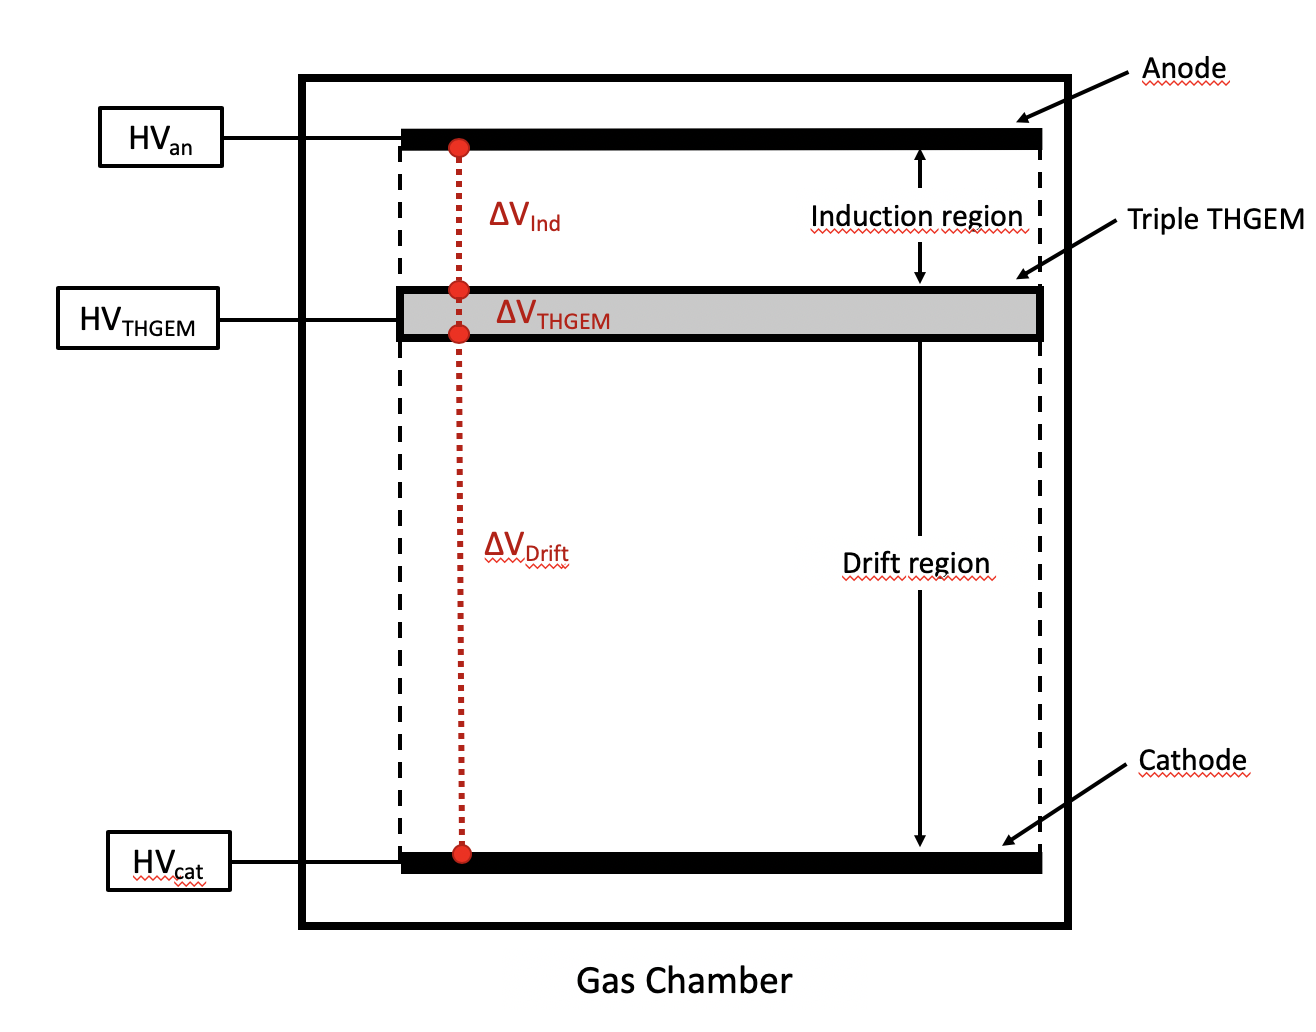
\includegraphics[width=0.9\textwidth]{Immagini/schema_apparato_2.png}
	\caption{Sketch of the Prototype.}
	\label{fig:schema_apparato_2}
\end{figure}

\subsection{THGEM}

Two multiple THGEM have been used in the test. Both of them are made of three layers, but they show 
different hole pattern and have been produced by two different manufacturers.\\
In the first one, referred to as FULL THGEM \textbf{F10} (Figure~\ref{fig:full_thgem}), the holes 
are uniformly distributed over the active surface; in the second one, called ROW THGEM \textbf{R1} 
(Figure~\ref{fig:row_thgem}), the holes are arranged in five rows.\\
The main characteristics of the two prototypes are shown in Table~\ref{tab:thgem}.\\

{\it Some comment on the differences of the two THGEM used for the test}.

\begin{table} [h!]
	\begin{center}
		\renewcommand{\arraystretch}{1.2}
\begin{tabular}{|c|c|c|}
\hline 
							& \textbf{F10} 		& \textbf{R1} \\ 
\hline 
Substrate material 			& Ceramic SD103K 	& PCB  \\ 
\hline 
Finish board thickness [mm] & 1.4 $\pm$ 0.1 	& 1.28 \\ 
\hline 
Dimension [$\mbox{mm}^2$] 	& 107$\times$107 	& 107$\times$107 \\ 
\hline 
Rim size [mm] 				& 0.1 				& 0.2  \\ 
\hline  
Rows 						& 143$\times$143 	& 5 \\ 
\hline 
Holes 						& 20449 			& 143 \\ 
\hline 
Hole diameter [mm] 			& 0.30 $\pm$ 0.05 	& 0.280 \\ 
\hline
Hole spacing 				& 0.75 				& 0.75 \\ 
\hline
\end{tabular} 
	\end{center}
	\caption{The main characteristics of the two type of THGEM tested.} \label{tab:thgem}
\end{table}

\begin{figure}
	\centering
		\subfigure[]{\label{fig:full_thgem}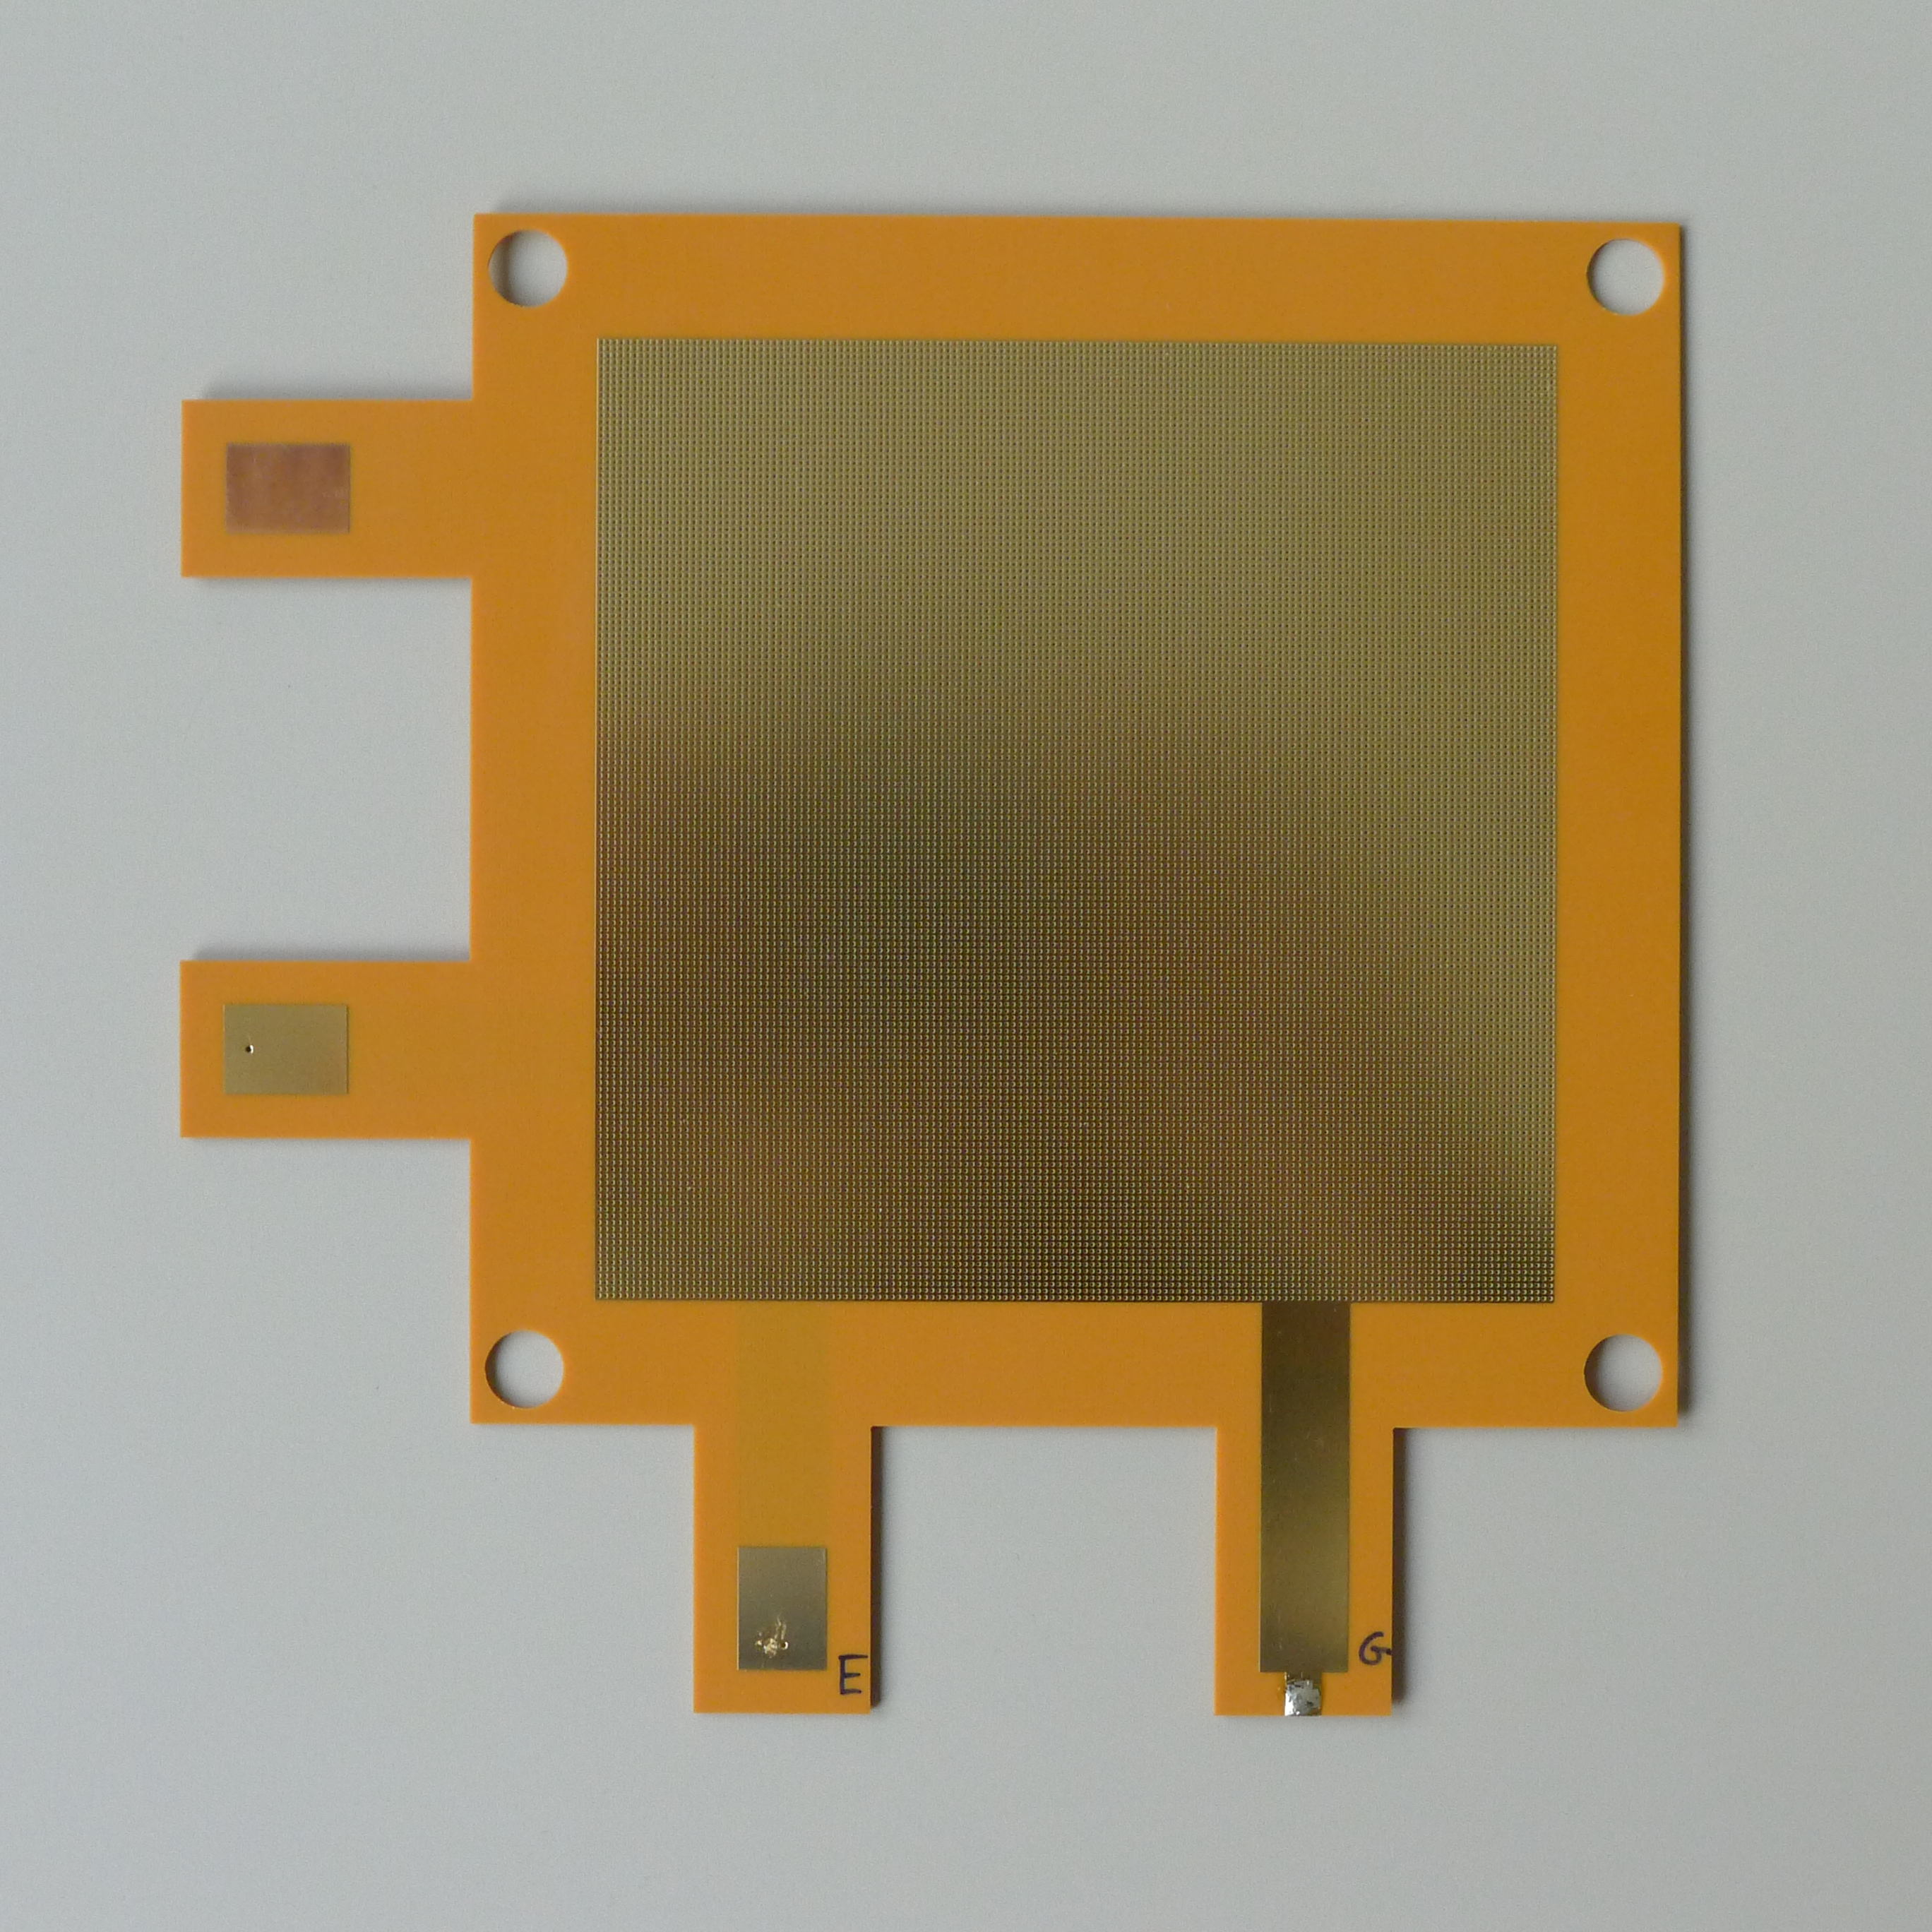
\includegraphics[width=0.45\textwidth]{Immagini/full_thgem.JPG}}
		\hspace{5pt}
		\subfigure[]{\label{fig:full_thgem_holes}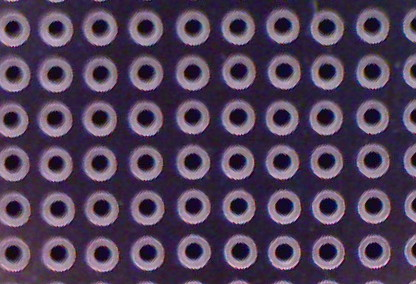
\includegraphics[width=0.45\textwidth]{Immagini/full_thgem_holes.JPG}}
	\caption{In (a) the FULL THGEM prototype, in (b) its hole pattern.}
	\label{fig:full_thgem_complessiva}		
\end{figure}

\begin{figure}
	\centering
	\subfigure[]{\label{fig:row_thgem}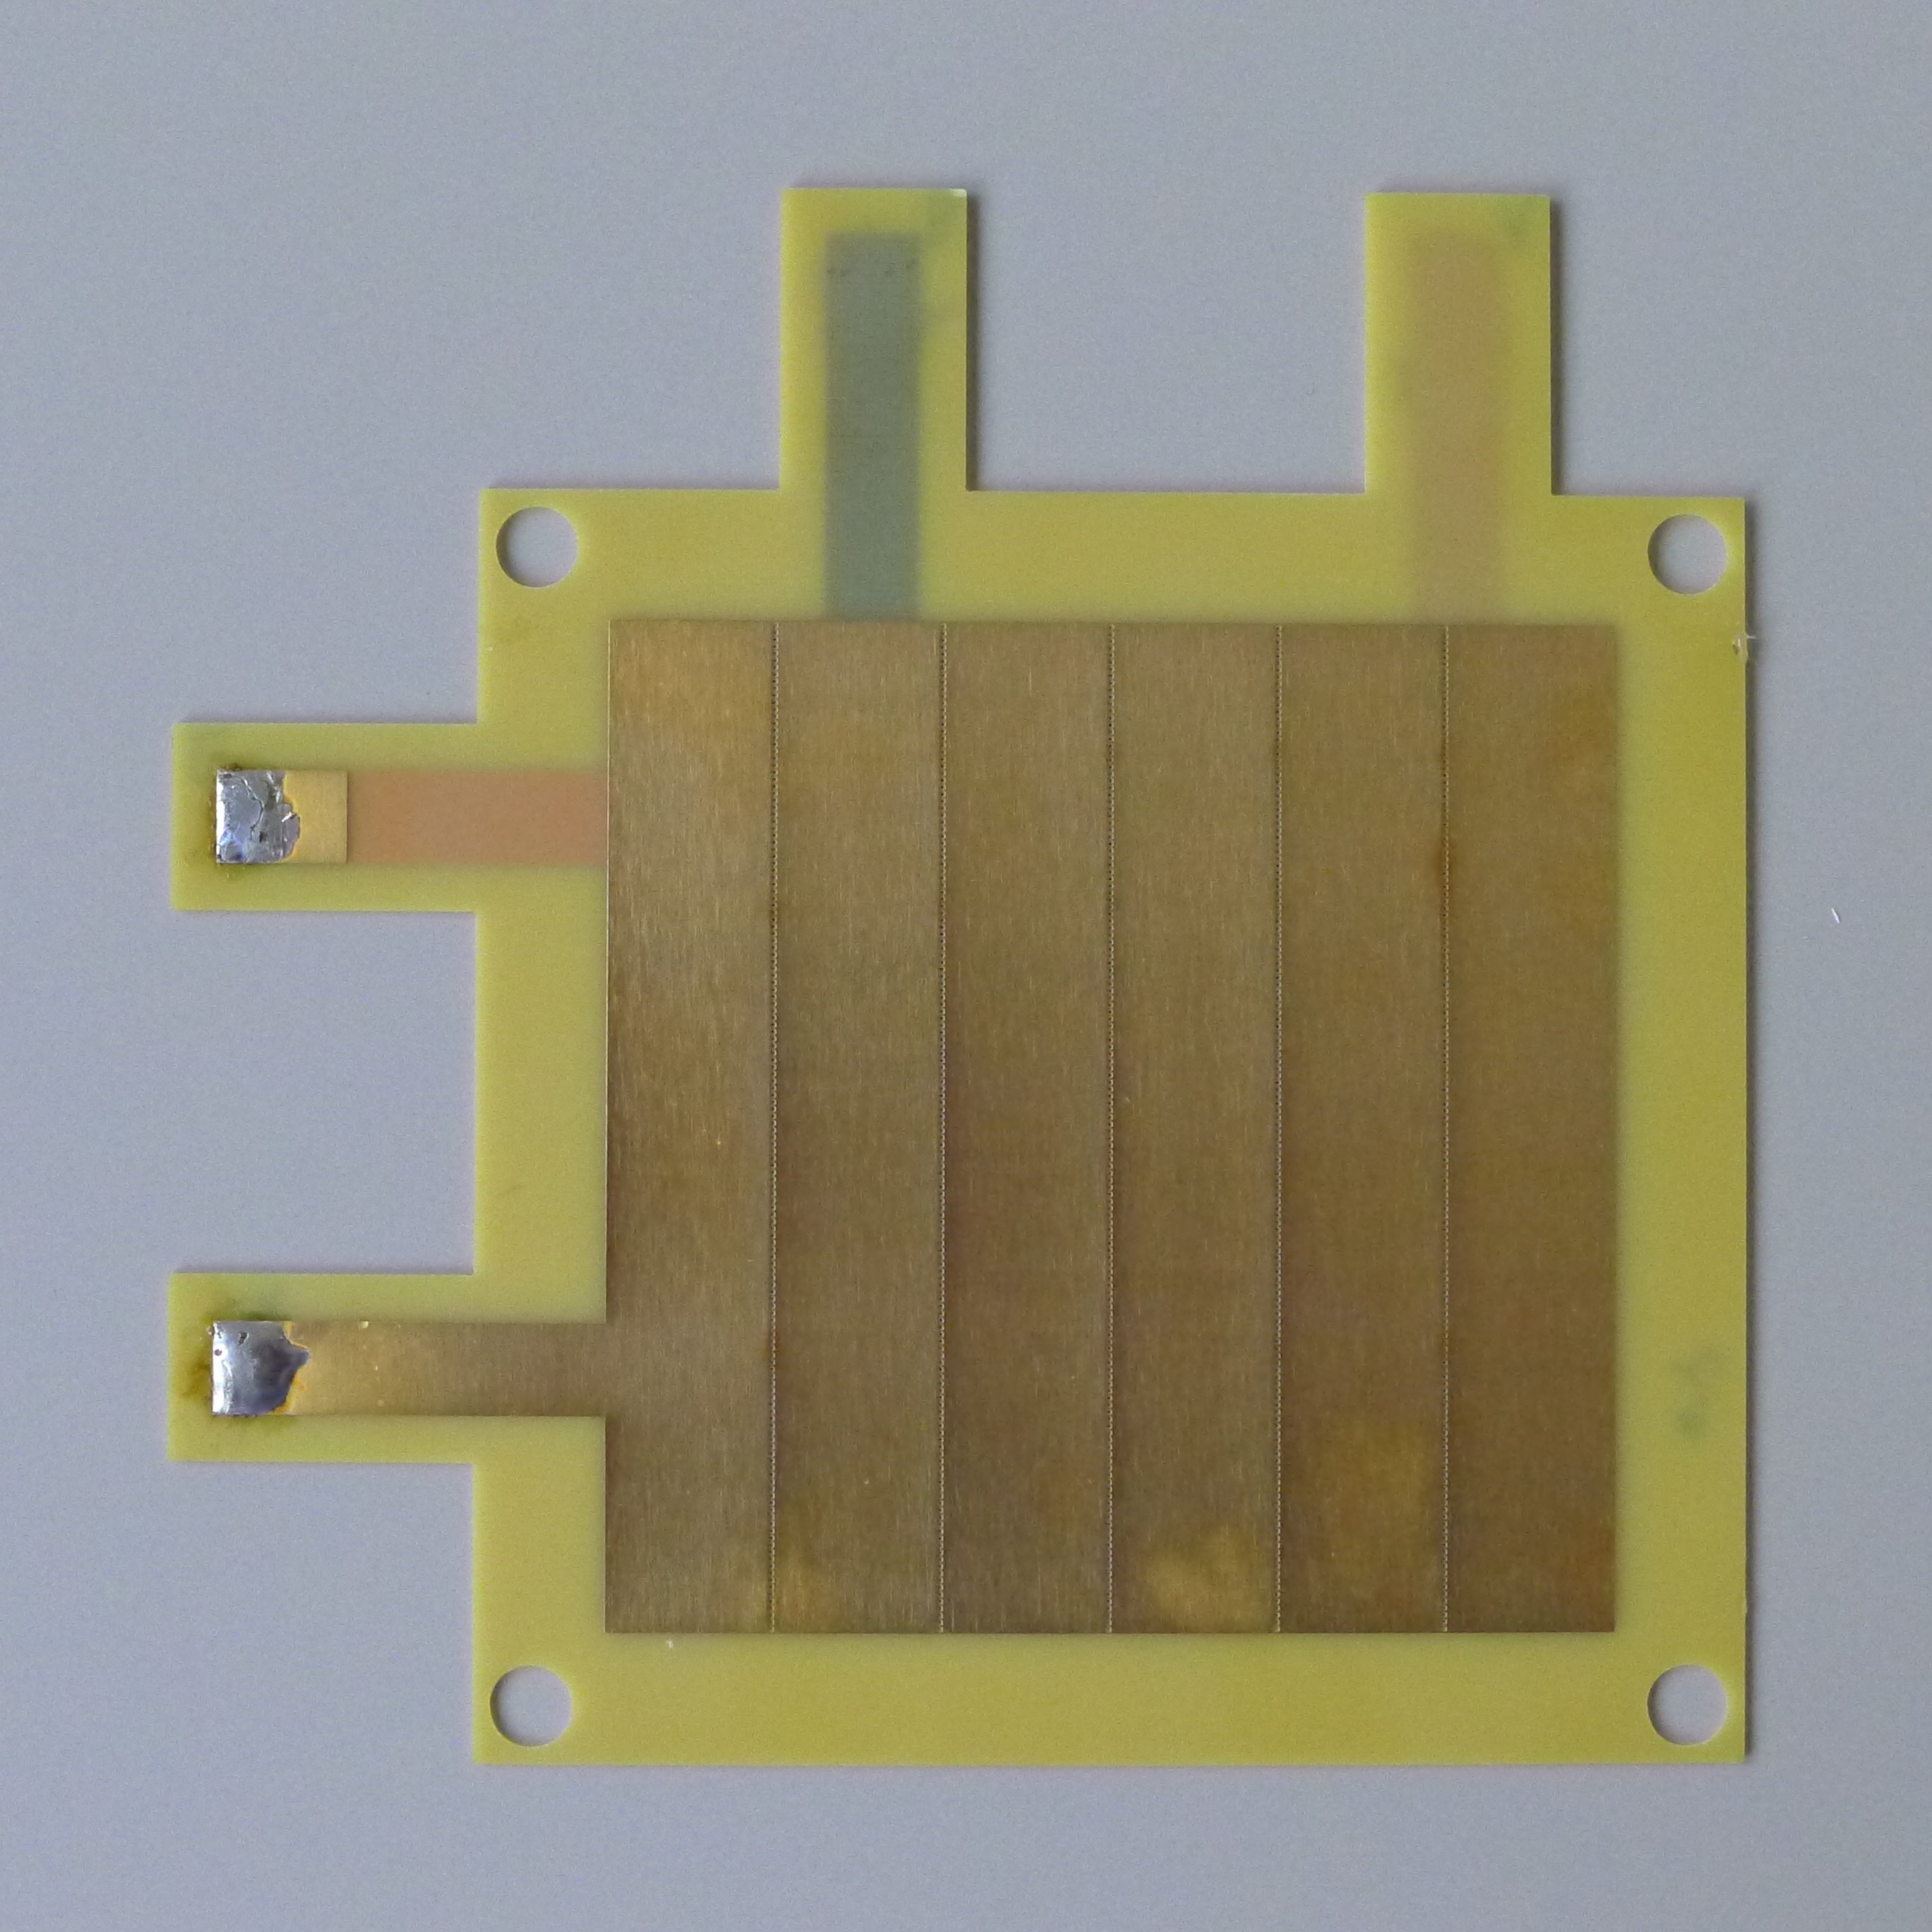
\includegraphics[width=0.45\textwidth]{Immagini/row_thgem.JPG}}
	\hspace{5pt}
	\subfigure[]{\label{fig:row_thgem_holes}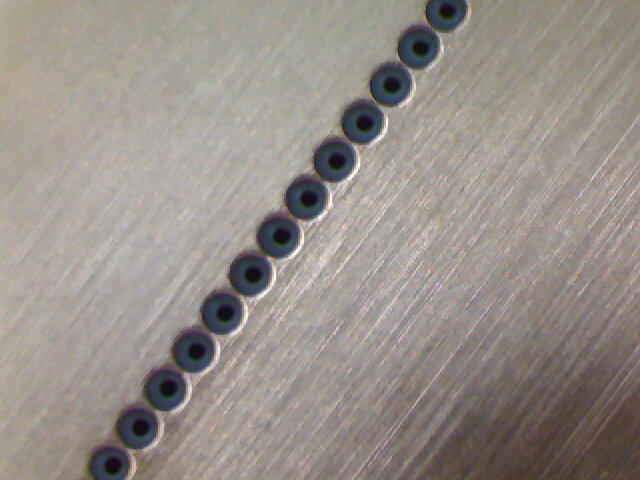
\includegraphics[width=0.45\textwidth]{Immagini/row_thgem_holes.JPG}}
	\caption{In (a) the ROW THGEM prototype, in (b) its hole pattern.}
	\label{fig:row_thgem_complessiva}		
\end{figure}

\subsection{The CAEN bias Supply and PICO}

The bias supply of the prototype is the CAEN SY5527 mainframe with an A1515 board.
A scheme of the bias is shown in Fig.~\ref{fig:

\begin{figure}[!htb]
	\centering
	\subfigure[]{ \label{fig:biasScheme1} \includegraphics[width=0.97\textwidth]{Immagini/
THGEM_Bias.pdf}}
	\subfigure[]{ \label{fig:biasScheme2} \includegraphics[width=0.97\textwidth]{Immagini/
THGEM_Bias_2.pdf}}
	\caption{Scheme of the Bias supply during the meausurements with electronics a) and for the current measurements b).}
	\label{fig:induction_FULLTHGEM_other_pressure}
\end{figure}



In in Figure~\ref{fig:run190_CAEN_pico} a comparison between the two ammeter is shown.  Both CAEN and PICO 
ammeter measure at the same time six currents: anode, top3, bot3/top2, bot2/top1, bot1 and cathode as shown in Figure~\ref{fig:schema_canali}. Top3 current is referred to the current value of THGEM electrode in front of the anode. Bot3/top2 current is related to the current collected between the third and the second THGEM of the Triple THGEM while bot2/top1 is referred to the current collected between the first and the second THGEM. Bot1 current is related to the current value of the THGEM electrode in front of the cathode.\\
The bot1 current measurement is less accurate than the other current measurements because the 
current flowing is larger than the other channels. Therefore the pico-ammeter PICO works with
a different dinamical range that has a lower accuracy.

\begin{figure}
	\centering
	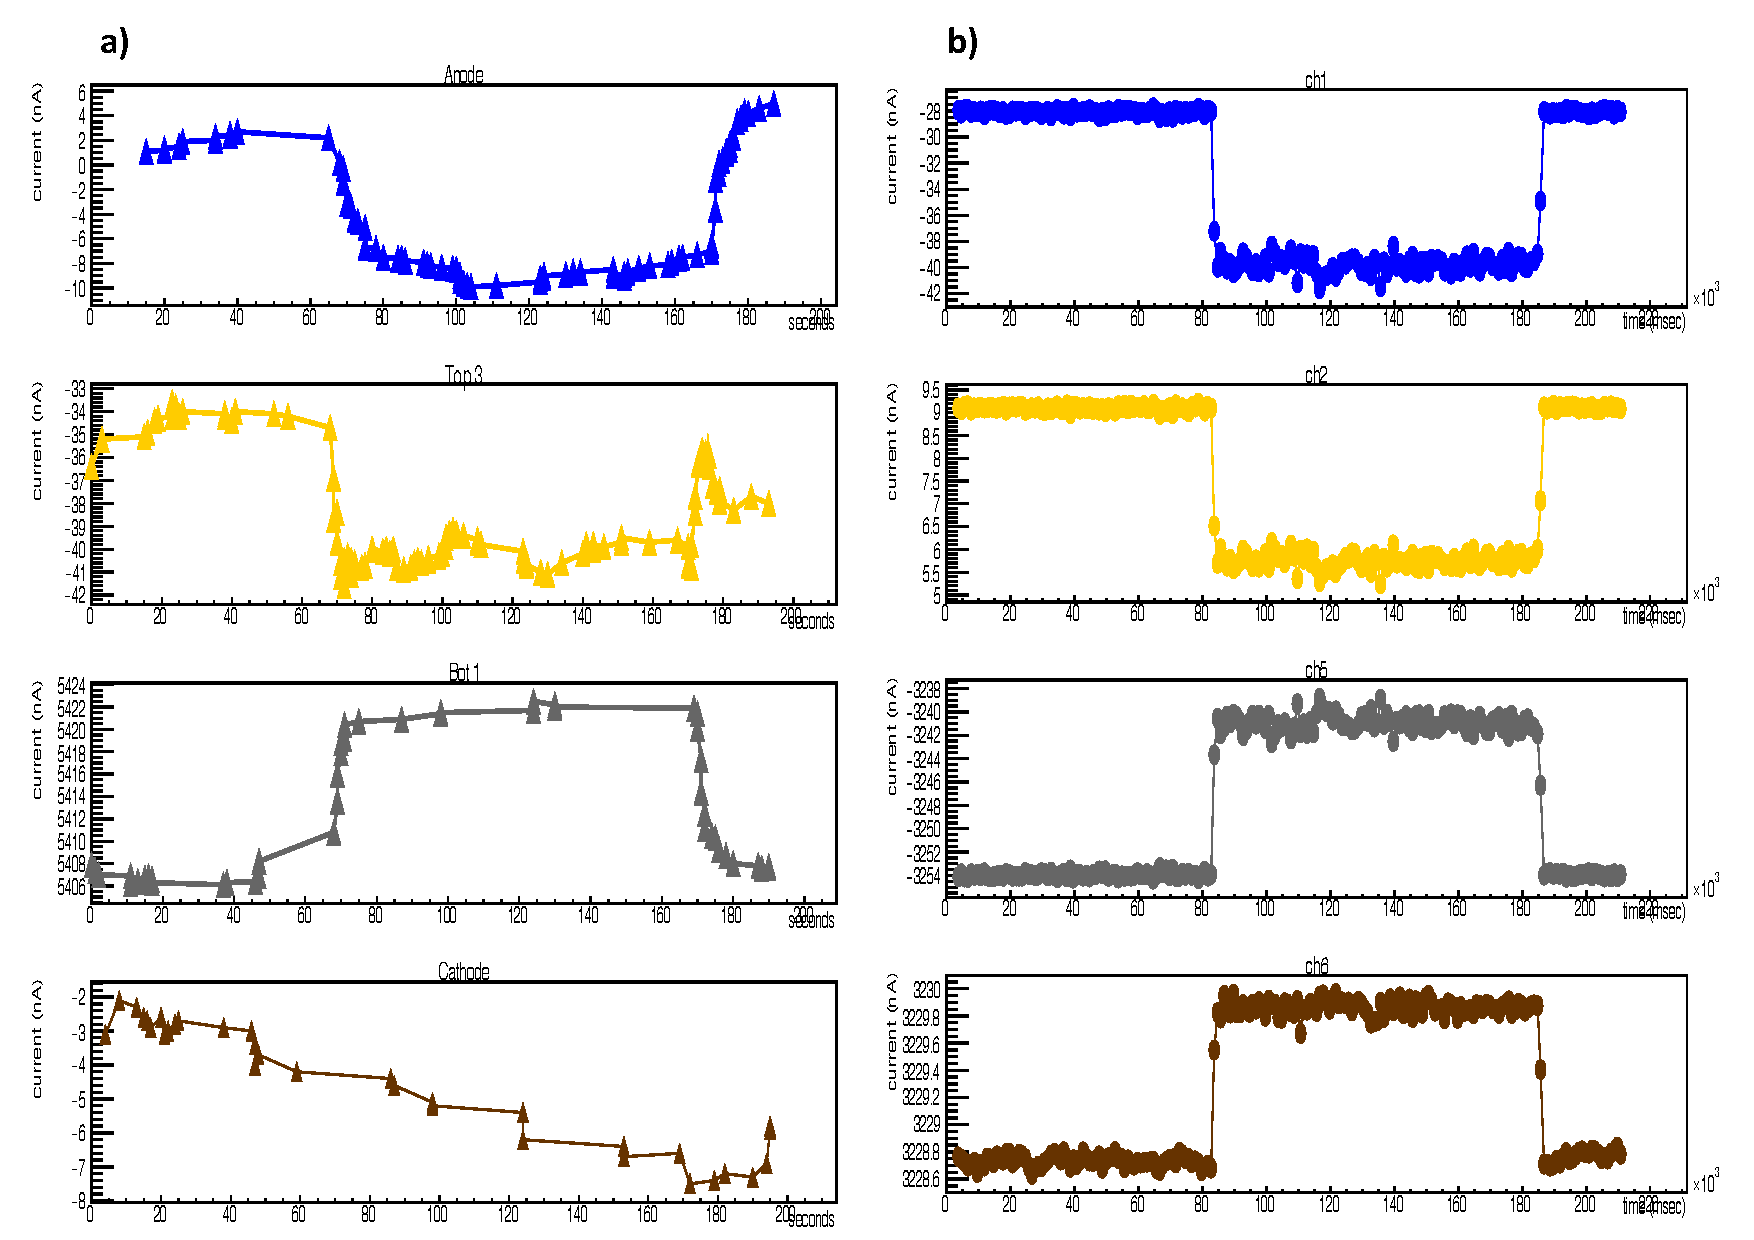
\includegraphics[width=1\textwidth]{Immagini/run190_CAEN_pico.pdf}
	\caption{Anode, Top3, Bot1 and Cathode currents measured with CAEN system a) and PICO b).}
	\label{fig:run190_CAEN_pico}
\end{figure}
\begin{figure}
	\centering
	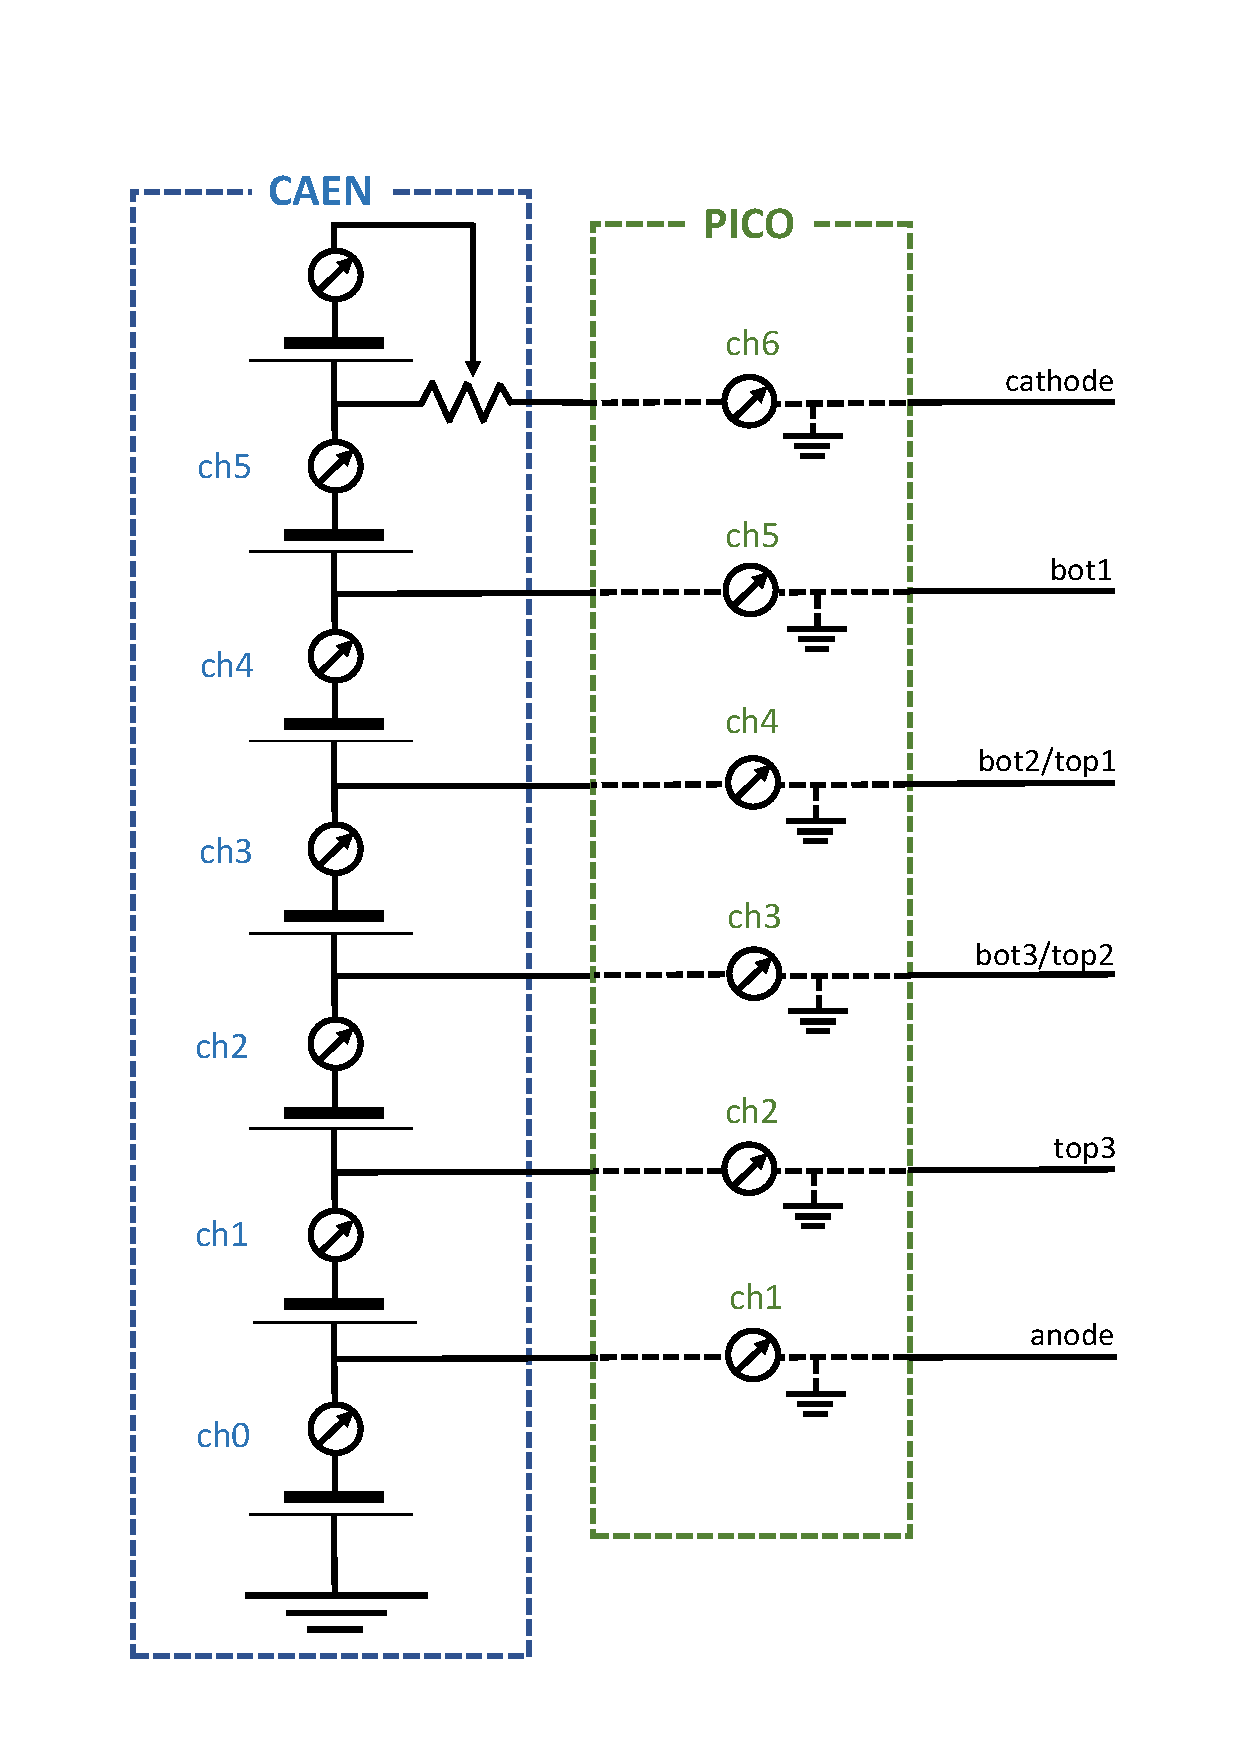
\includegraphics[width=0.8\textwidth]{Immagini/schema_canali.pdf}
	\caption{Current reading scheme for the two ammeters.}
	\label{fig:schema_canali}
\end{figure}

\section{Method}

The main parameters that determine the behaviour of the detector are: gas pressure, voltage of the 
THGEM (V$_{THGEM}$), voltage of the induction region (V$_{ind}$) and voltage of the drift region 
(V$_{drift}$).

The method consists in keeping fix all the parameter but one and to measure all the currents of 
all the electrodes varying just the parameters let free to change.
For example we keep fix the gas pressure the V$_{drift}$, V$_{ind}$, while the V$_{THGEM}$) was
changed a small step. In this way we get 6 plot currents as a function of V$_{THGEM}$).

In order to measure the current of the anode, this last cannot be kept at ground therefore the 
anode was kept at voltage fixed to an arbitrary value of 20~V that should not affect the 
measurements of the currents of any electrodes. 
For example, during the $\Delta V_{ind}$ scan, the $\Delta V_{THGEM}$ and $\Delta_{drift}$ were fixed and 
anode, bot1, top3 and cathode currents were MEASURED (see Figure~\ref{fig:schema_canali}).\\
A run lasts usually 180 s (see Fig. \ref{fig:fig:run190_CAEN_pico}):\\
60 s with shutter closed;\\
90 s with shutter open;\\
30 s with shutter closed.\\
An average of the current flowing during the first 60 s (shutter closed) and an average during
the 90 s with shutter open is performed.
The difference between the two measurements with shutter open and closed give
 the actual current associated to the $\alpha$-particles entering the detector.
In this way any dark current coming from the detector or from the ammeter is subtracted\footnote{A possible source of
dark current is due to the X-ray produced by the $\alpha$-source that are not stopped by the shutter.}.\\

\clearpage

\section{Measurements}

%i canali 3 e 4 possono essere ignorati perche non danno mai segnale

%spieghiamo i diversi scan (induzione, thgem e drift)

%In this section the results of 

%For the sake of clarity

\subsection{FULL THGEM}

\subsubsection{Scan on \Vind}

%The scan on \Vind aimed at studying the behaviour of 

%A preliminary study of \Vind{} variation effects on the measured currents has been done at several pressure and setting different \Vthgem{} and \Vdrift{} values.
A series of systematic measurements were performed to study the effects of the variation of the potential difference \Vind{} on all the measured currents.
These measurements were done at different pressures (P) and values of \Vthgem{} and \Vdrift{},
a summary scheme of the configurations is shown in Table~\ref{tab:FULLTHGEM_vind}.
\begin{table} [b!]
	\begin{center}
		\renewcommand{\arraystretch}{1.2}
		\begin{tabular} {ccccc}
			P (mbar) & & \Vthgem{} (V) & & \Vdrift{} (V)\\
			\toprule[0.1em]
			%\hline
			30	& &	220	& &	1000 \\
			30	& &	200	& &	1000 \\
			30	& &	230	& &	1000 \\
			20	& &	200	& & 1000 \\
			11	& & 170	& & 600 \\
			
			\bottomrule[0.1em]
		\end{tabular}
	\end{center}
	\caption{The values of pressure (P), \Vthgem{} and \Vdrift{} adopted for the study on \Vind.} \label{tab:FULLTHGEM_vind}
\end{table}
%\begin{table} [b!]
%	\begin{center}
%		\renewcommand{\arraystretch}{1.2}
%		\begin{tabular} {ccccccc}
%			P (mbar) & & \Vthgem{} (V) & & \Vdrift{} (V) & & optimal \Vind{} (V) \\
%			\toprule[0.1em]
%			%\hline
%			30	& &	220	& &	1000 & & 120 \\
%			30	& &	200	& &	1000 & &  \\
%			30	& &	230	& &	1000 & & \\
%			20	& &	200	& & 1000 & & \\
%			11	& & 170	& & 600  & &\\
%			
%			\bottomrule[0.1em]
%		\end{tabular}
%	\end{center}
%	\caption{The values of pressure (P), \Vthgem{} and \Vdrift{} adopted for the study on \Vind.} \label{tab:FULLTHGEM_vind}
%\end{table}
The \Vind{} scans were carried out starting from 0~V and increasing the voltage by 10 or 20~V per run, until the discharge value is reached.
This value is dependent on the gas pressure and possibly on the values set for \Vthgem{} and \Vdrift.
The values at which discharge occurs are 220, 200 and 150 V for 30, 20 and 11 mbar respectively.\\

A typical example of the scan is shown in Figure~\ref{fig:induction_FULLTHGEM_30mbar}, it corresponds
at 30~mbar and \Vthgem{}~=~220~V. By raising the value of \Vind{}, the anodic current (blue line) 
increases, while the top3 current (yellow line) decreases approaching zero.
\begin{figure}[!t]
	\centering
	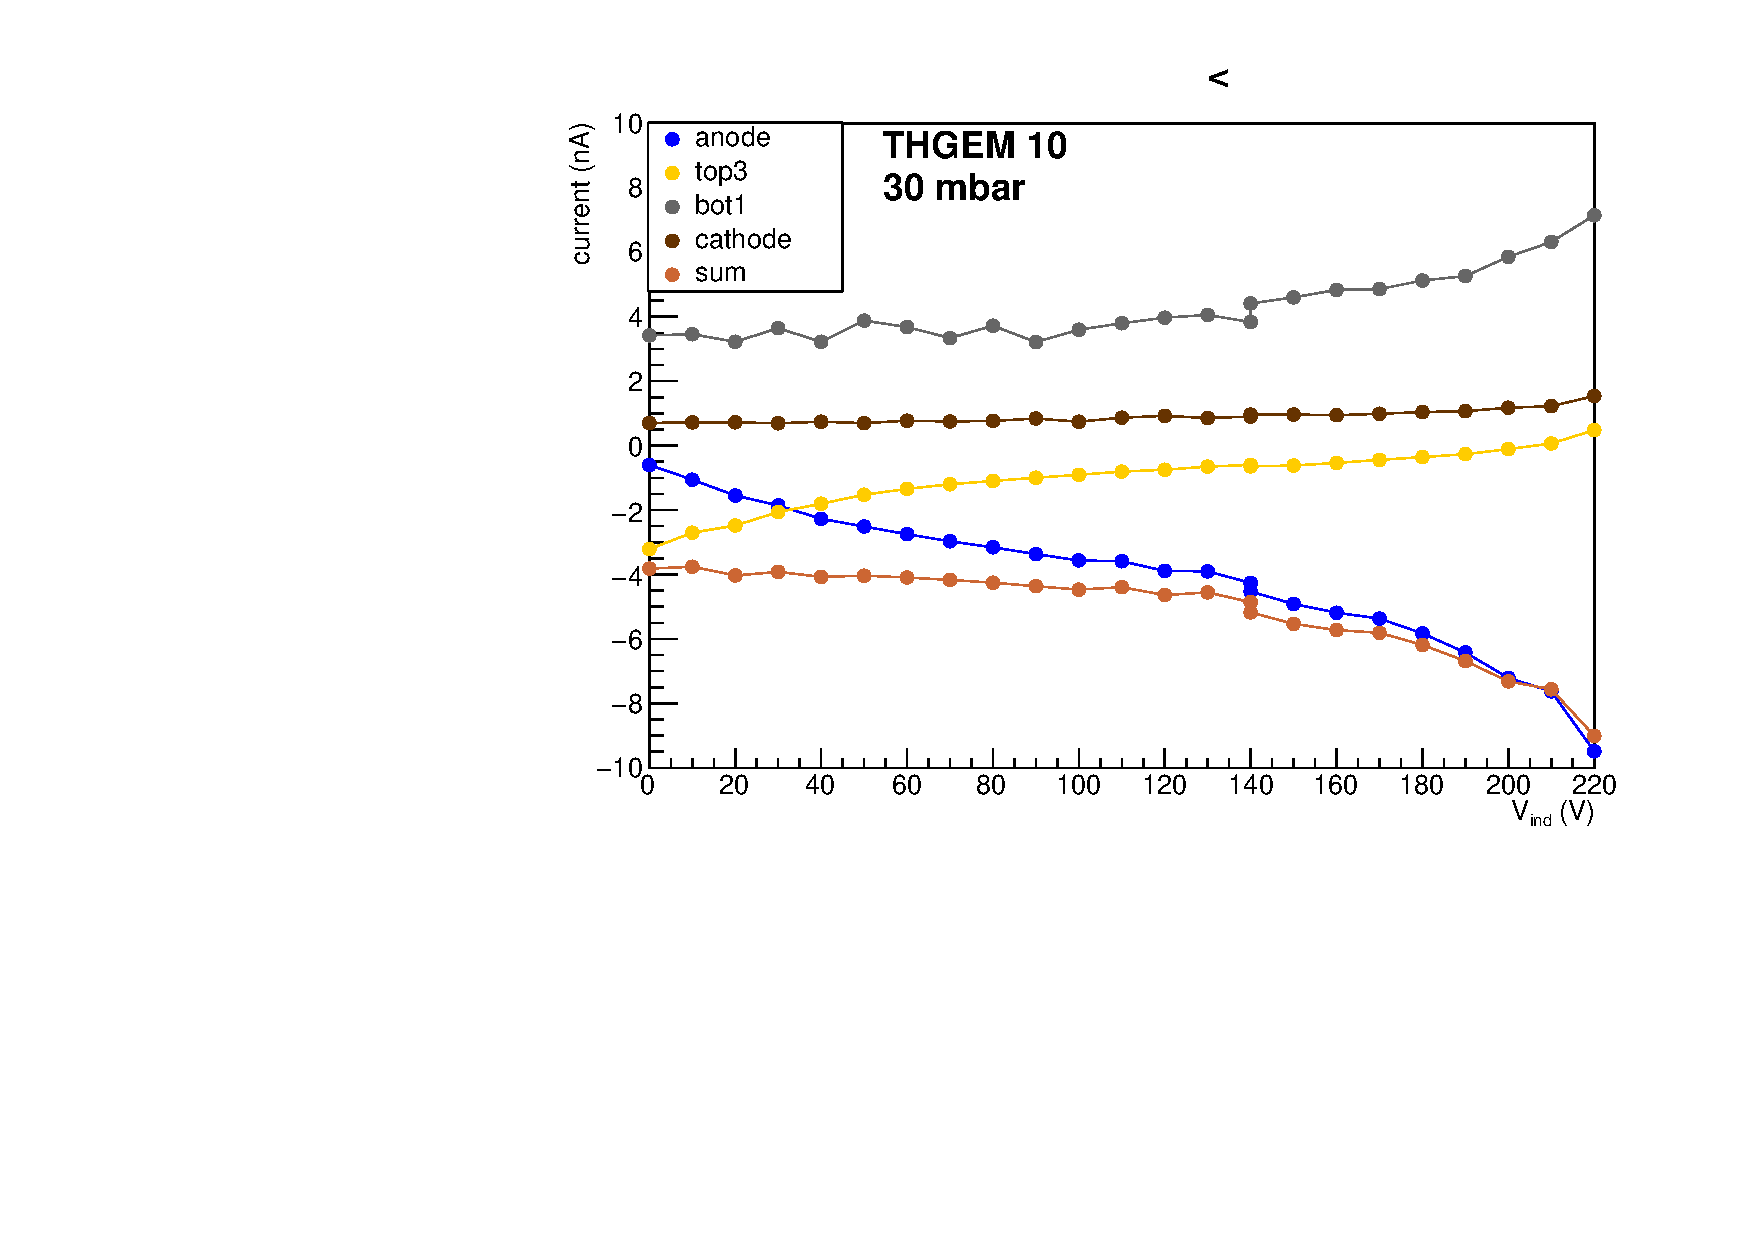
\includegraphics[width=\textwidth]{Immagini/inductionScan_THGEM10_30mbar.pdf}
	\caption{Currents measured during the scan on the voltage \Vind{} across the induction region at 
	30~mbar and with \Vthgem{}~=~220~V.}
	\label{fig:induction_FULLTHGEM_30mbar}
\end{figure}
The orange points corresponds to the sum of the currents read in top3 and anode, that is to the total 
negative charge (TNC) produced by the THEGEM. Up to 140~V, The TNC is approximately constant.
% but their change is such that their sum (orange line) is constant.
%Up to 140~V, when \Vind{} increases, the anodic current (blue line) goes up, the top3 current (yellow line) approaches to zero, and their sum (orange line) is constant.
This simply means that the stronger is the electric field in the induction region, the greater is 
the fraction of secondary electrons collected at the anode.
%Up to 140~V, the sum of anode and top3 currents (orange line) is constant, so the 
%The total number of secondary electrons, 
%The sum of anode and top3 currents is constant 
%; in particular, for \Vind{} greater than about 30~V most electrons
%This means that when the electric field in the induction region is weak, most of the electrons produced by multiplication are collected at the top3 electrode and only a few reaches the anode.
For \Vind{} greater than 140~V, the TNC increases: this behaviour can be explained considering 
that, when the voltage is high enough, the multiplication region extends out of the THGEM holes, 
expanding in the induction region (see Fig.~\ref{fig:induction_FULLTHGEM_30mbar_other_VTHGEM}
for a more evident effect.).
For values of \Vind{} equal to 220~V, the top3 current becomes positive, This could be explained
supposing that a fraction of the positive ions produced in  are collected by the top3 electrode.
In these conditions, the chosen operational value is \Vind{} is 120~V, this value ensure that a 
large fraction of the electron is collected on the anode and that the multiplication is
mainly confined on the THGEM holes.

At the pressure of 30 mbar the scan was repeated with two different values of \Vthgem{}: namely 200 
and 230 V (see Fig~\ref{fig:induction_FULLTHGEM_30mbar_other_VTHGEM_a,fig:induction_FULLTHGEM_30mbar_other_VTHGEM_b}.
\begin{figure}[!htb]
	\centering
	\subfigure[]{ \label{fig:induction_FULLTHGEM_30mbar_other_VTHGEM_a} 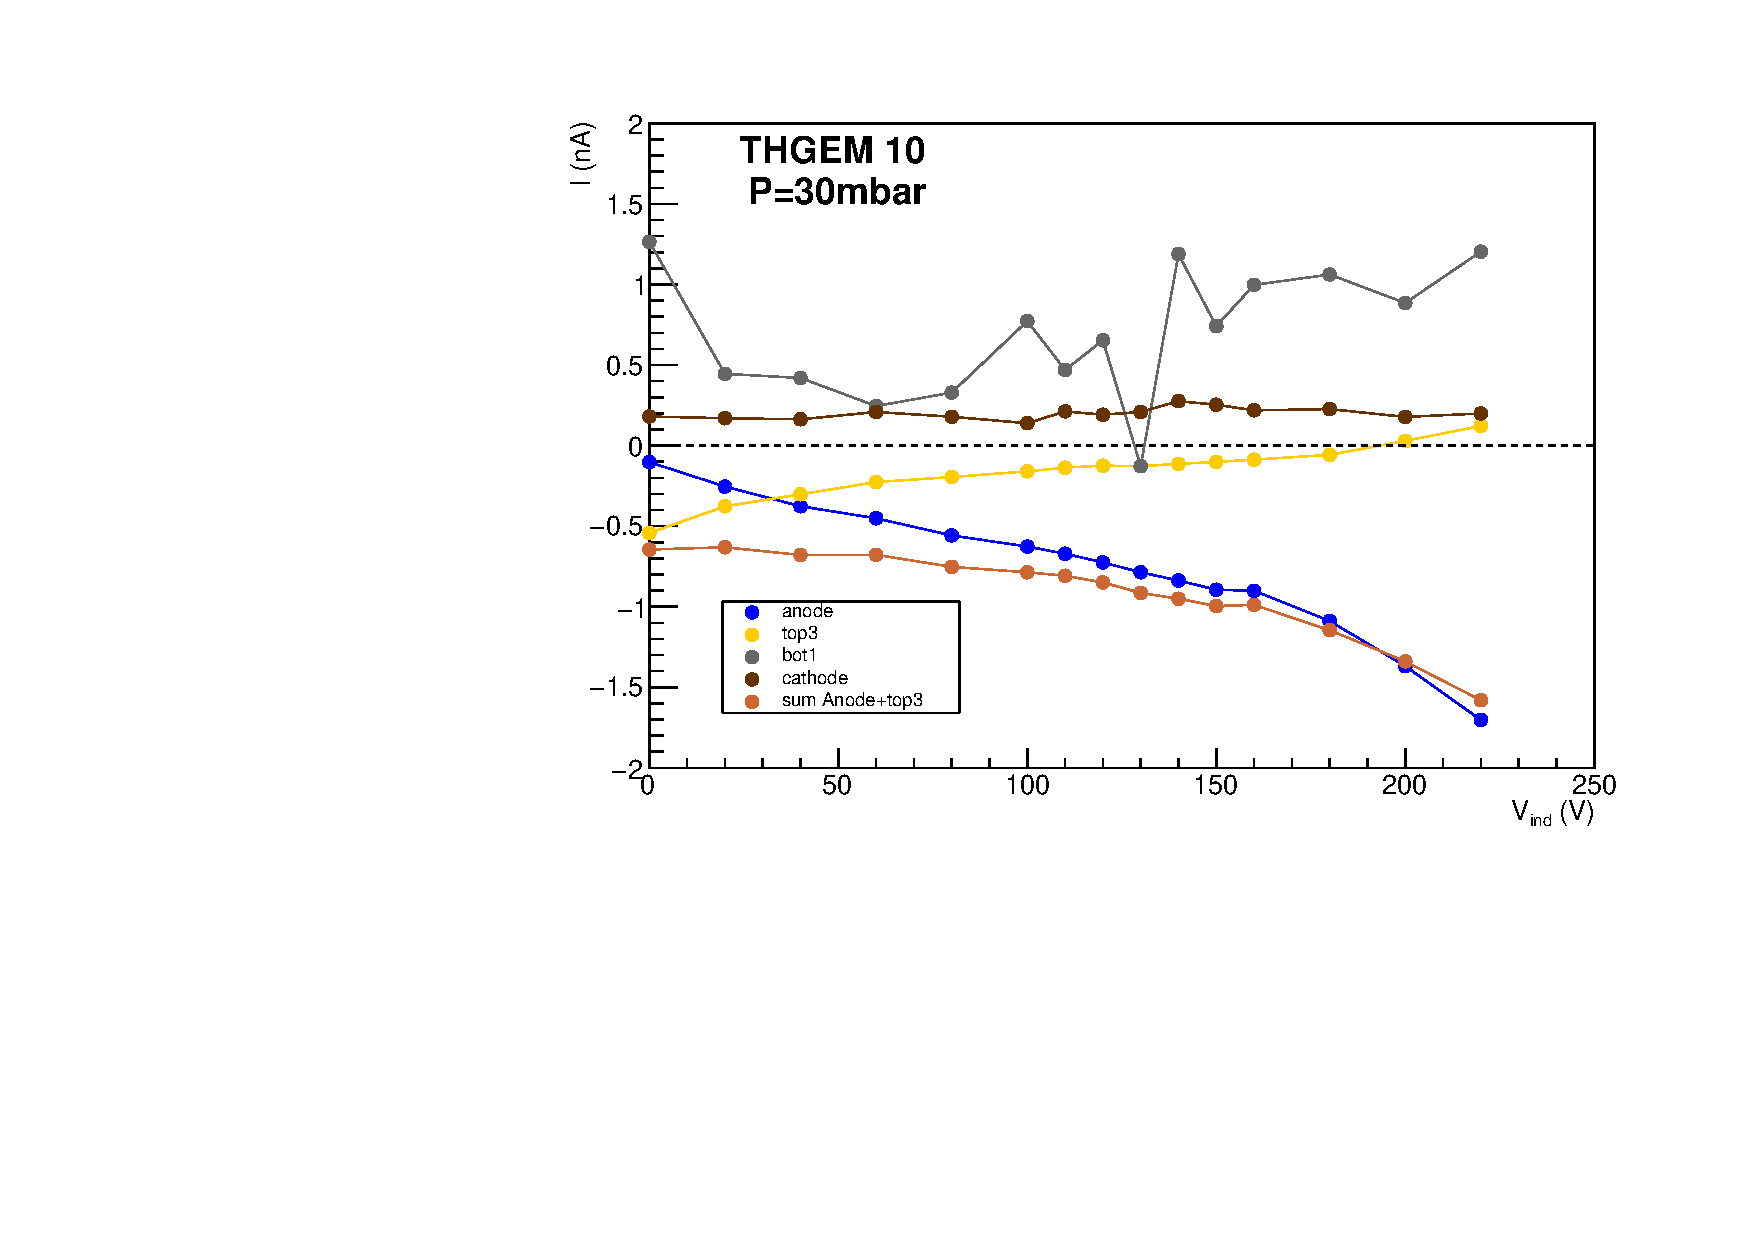
\includegraphics[width=0.96\textwidth]{Immagini/inductionScan_THGEM10_30mbar_bis.pdf}}
	\subfigure[]{ 	\label{fig:induction_FULLTHGEM_30mbar_other_VTHGEM_b} 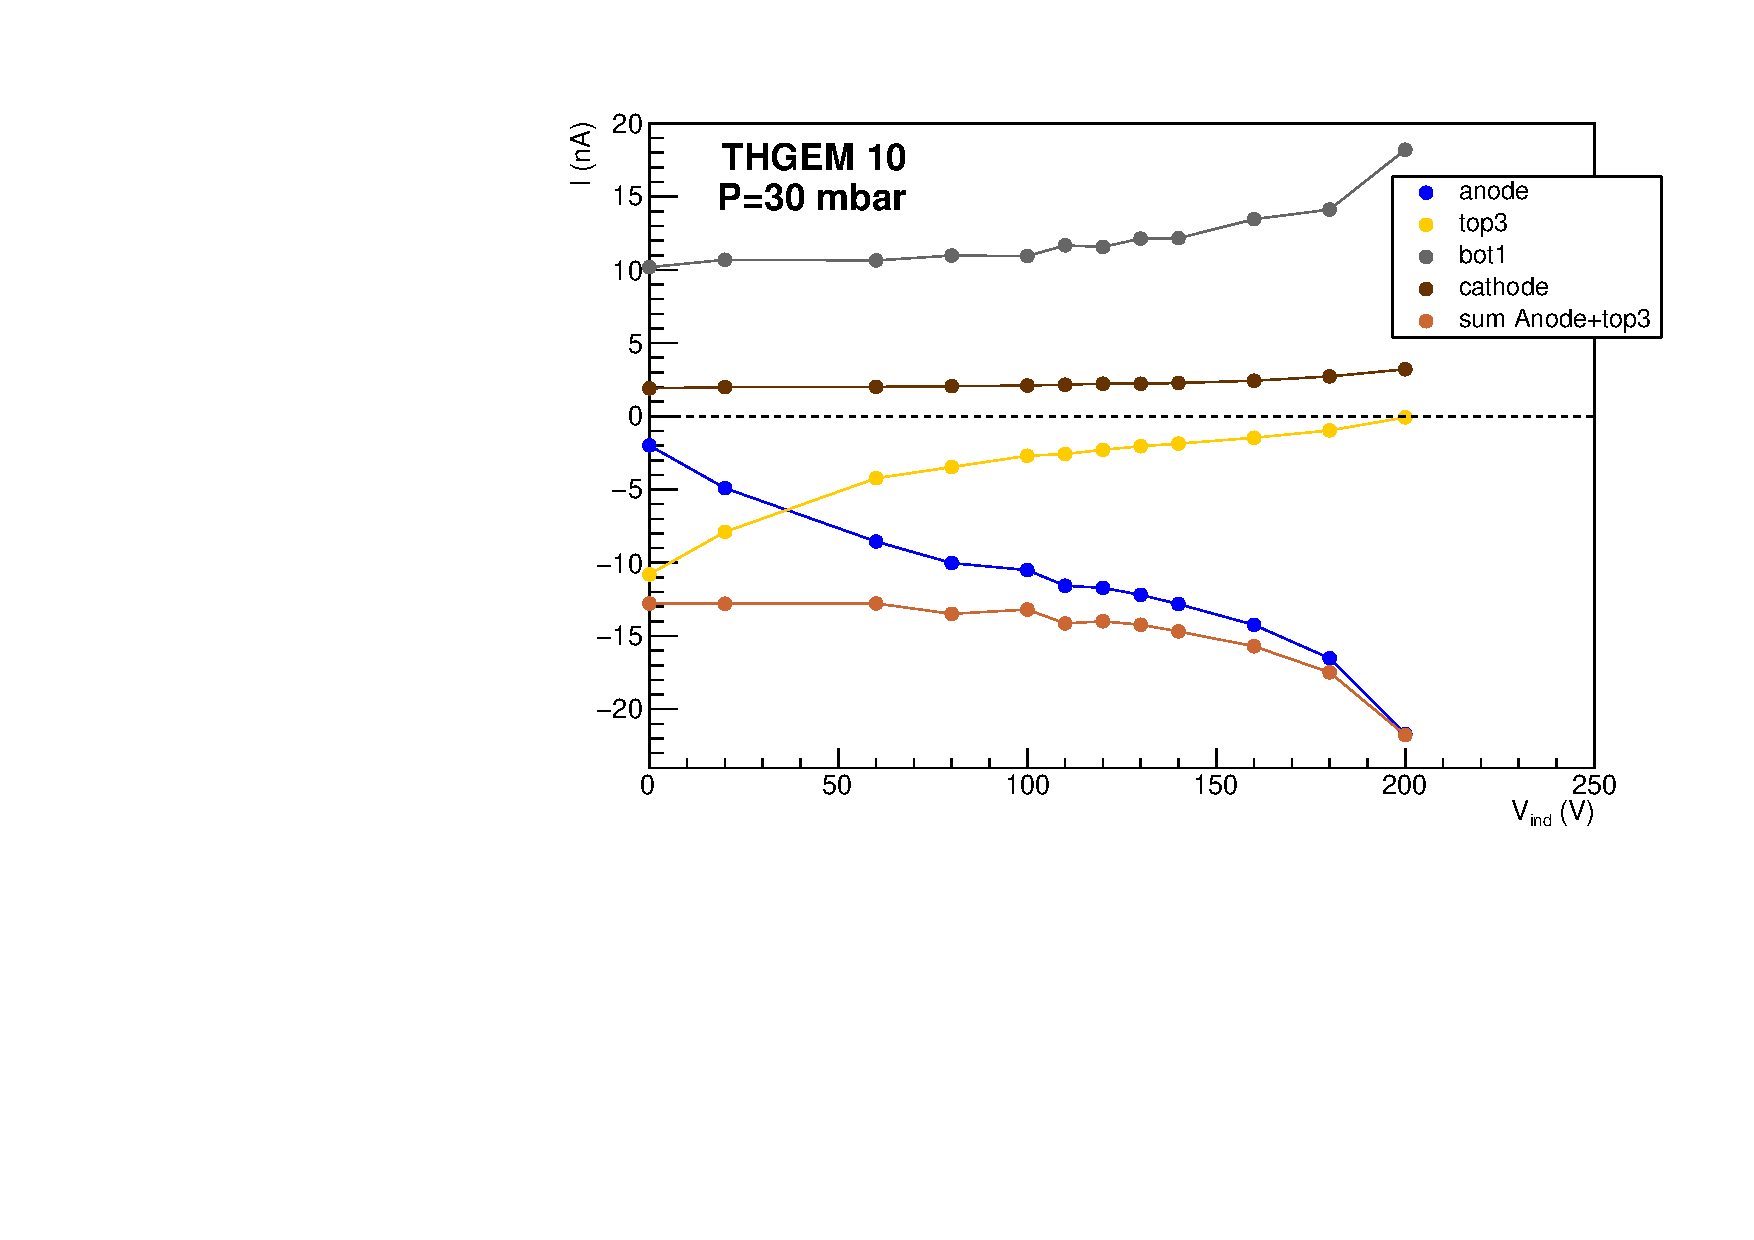
\includegraphics[width=0.96\textwidth]{Immagini/inductionScan_THGEM10_30mbar_tris.pdf}}
	\caption{Currents measured during the scan on the voltage \Vind{} across the induction region at 30~mbar: in (a) for \Vthgem~=~200~V, in (b) for \Vthgem~=~230~V. In a) the bot1 current fluctuations are due to the lower accuracy of the corresponding PICO channel.
}
	\label{fig:induction_FULLTHGEM_30mbar_other_VTHGEM}
\end{figure}

The scans at 20 and 11 mbar shown in Figure~\ref{fig:induction_FULLTHGEM_20mbar} and~\ref{fig:induction_FULLTHGEM_11mbar}.

\begin{figure}[!htb]
	\centering
	\subfigure[]{ \label{fig:induction_FULLTHGEM_20mbar} 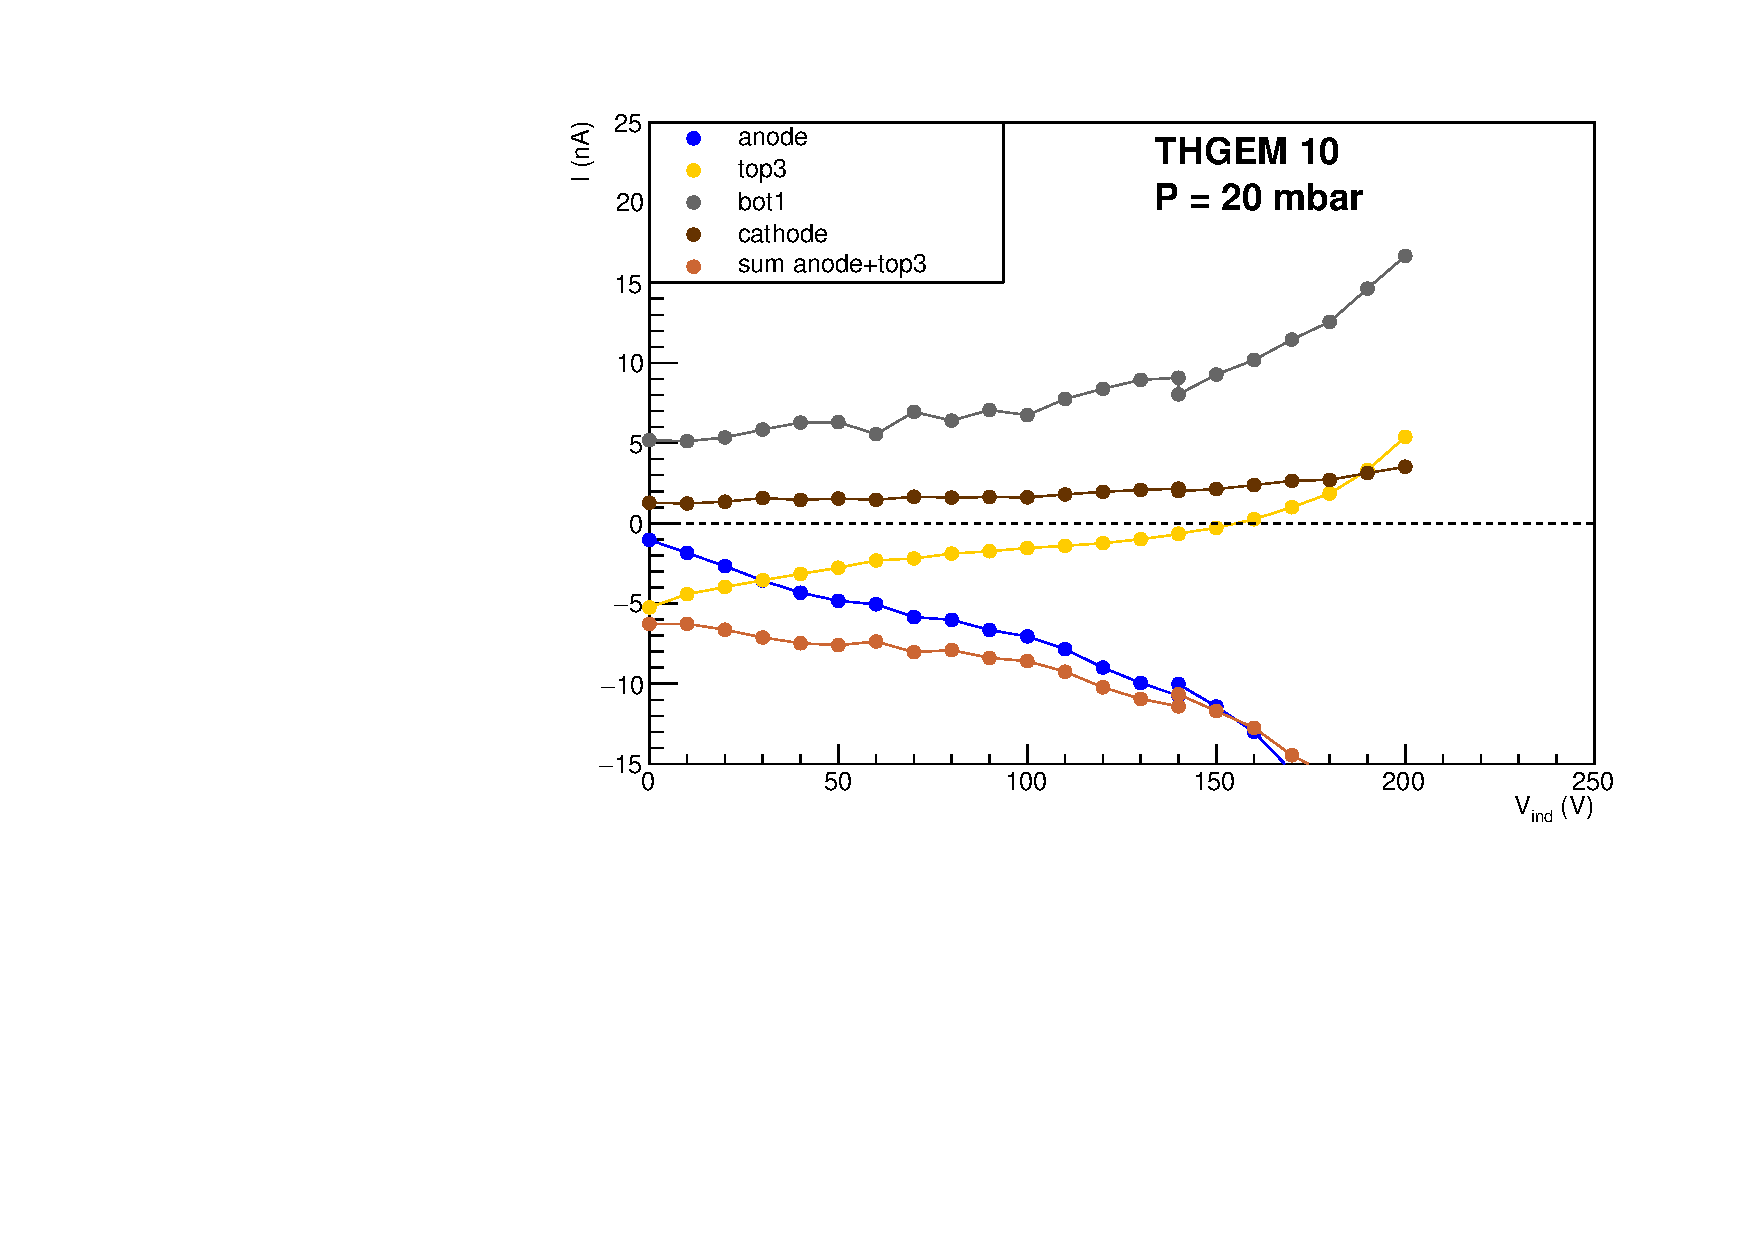
\includegraphics[width=0.97\textwidth]{Immagini/inductionScan_THGEM10_20mbar.pdf}}
	\subfigure[]{ \label{fig:induction_FULLTHGEM_11mbar} 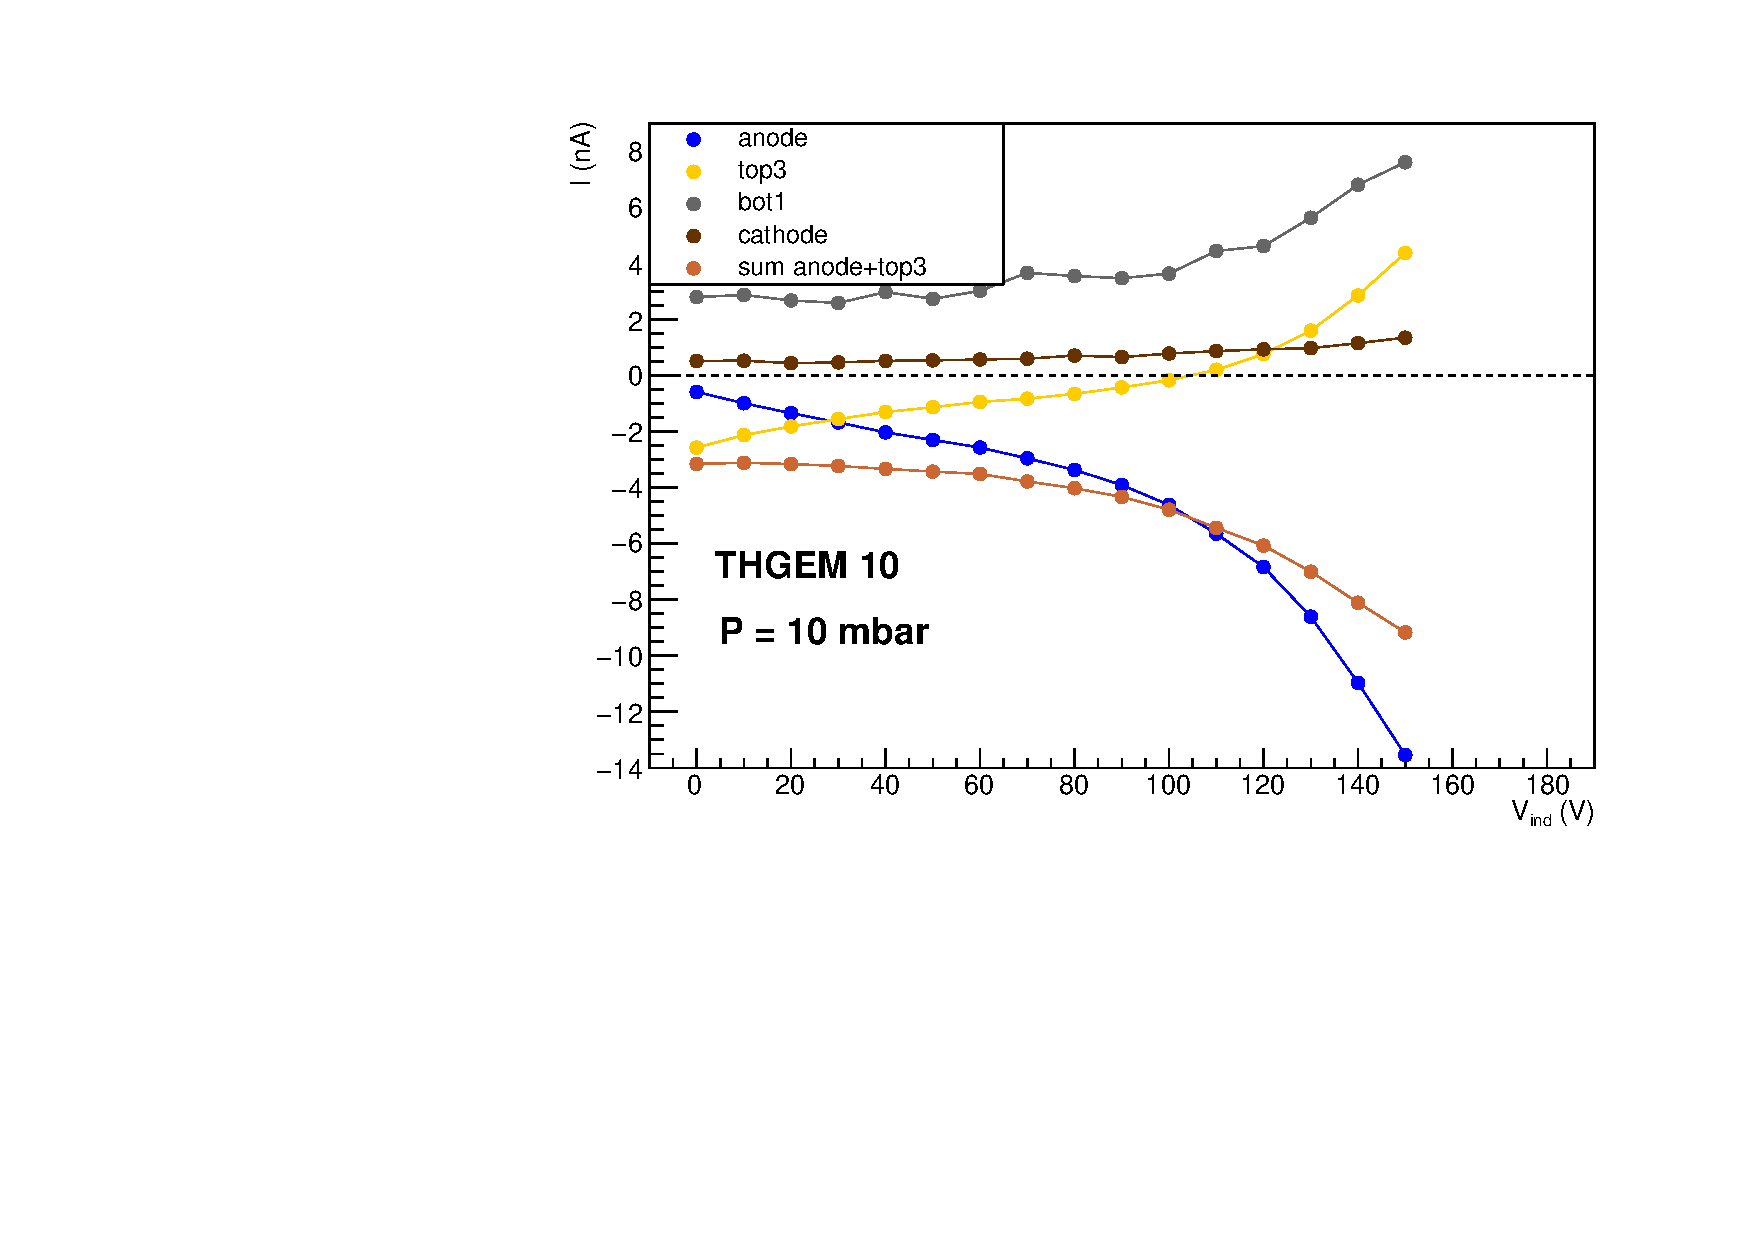
\includegraphics[width=0.97\textwidth]{Immagini/InductionScan_THGEM10_10mbar_tris.pdf}}
	\caption{Currents measured during the scan on the voltage \Vind{} across the induction region: in (a) at 20~mbar, in (b) at 11~mbar.}
	\label{fig:induction_FULLTHGEM_other_pressure}
\end{figure}

%Also in these two measurements, when \Vind{} increases, the anodic current increases, while the top3 current decreases. The crossing point of these two currents is still at around 32~V. After a certain value the sum of the anode and top3 current varies rapidly.

%The effects seen for \Vthgem~=~220~V appear as well in these two cases.
%The magnitude of the measured currents increases with increasing \Vthgem, because
%For \Vthgem~=~200~V the magnitude of the measured currents is lower than in the previous case, while for \Vthgem~=~230~V it is 

%as expected, increasing \Vind{} the fraction of electrons collected at the anode
%this plot displays some of the most important features



%\subsubsection*{Scan on induction voltage at 30 mbar}
%To find the optimal value for the induction voltage, a scan on this parameter has been done. The measured currents obtained for a pressure of 30~mbar and for \Vthgem~=~220~V and \Vdrift~=~1000~V are shown in Figure~\ref{fig:induction_FULLTHGEM_30mbar}. In each plot, bot2/top1 and bot3/top2 currents are not shown because their values do not change during the measurement. In Figure~\ref{fig:induction_FULLTHGEM_30mbar} is shown the sum of the anode and top3 currents. This curve has a plateau zone in the range 110$\div$130~V, so the optimal value for the \Vind is 120~V. The induction scan was repeated with \Vthgem~=~200~V and \Vthgem~=~230~V, but there was no visible plateau. In each induction scan, when the set voltage exceeds a certain value (different in the three cases), the sum of anode and top3 currents increases. This behaviour can be explained because the multiplication region extends out of the hole of the THGEM. The electric field gives a further multiplication and some ions reach the THGEM.

\clearpage

\subsubsection{Scan on \Vthgem}

The scan of \Vthgem{} have been performed keeping fix the \Vind{} and \Vdrift{}. 
%In order to study the multiplication factor of the FULL THGEM in different conditions, a series of measurements was conducted varying the voltage \Vthgem, while pressure, \Vind{} and \Vdrift{} were set to fixed values.
%The explored range of \Vthgem{} was determined in thi/inductionScan_THGEM10_10mbar_tris.pdf}s way: the lower extreme is the minimum value at which a variation of the measured currents is visible, while the higher extreme is the discharge value.
%The explored range of \Vthgem{} was determined in this way: the lower extreme is the minimum value at which, when opening the shutter, we see a variation of the measured currents; the higher extreme is the discharge value.
The \Vthgem{} was explored from 0 to a maximum value before the discharge occurs at step of 5/10 V. 
%for P~=~30 mbar it was from 180 to 235~V, for P~=~20~mbar it was from 150 to 215~V, and for P~=~11~mbar a it was from 130 to 210~V.
%The increments were ranging from 5 to 10~V.
Table~\ref{tab:FULLTHGEM_vthgem} shows the configurations of the scans.

\begin{table} [!h]
	\begin{center}
		\renewcommand{\arraystretch}{1.2}
		\begin{tabular} {ccccccc}
			P (mbar) & & \Vind{} (V) & & \Vdrift{} (V) & & \Vthgem{} range (V)\\
			\toprule[0.1em]
			%\hline
			30	& &	120	& &	1000	& & 180$\div$235 \\
			20	& &	100	& & 1000	& & 150$\div$215 \\
			11	& & 70	& & 600		& & 130$\div$210 \\
			
			\bottomrule[0.1em]
		\end{tabular}
	\end{center}
	\caption{P, \Vind{}, \Vdrift{} and the explored \Vthgem{} range used in the \Vthgem{} scans.} \label{tab:FULLTHGEM_vthgem}
\end{table}

Figure~\ref{fig:thgem_FULLTHGEM_30mbar}, \ref{fig:thgem_FULLTHGEM_20mbar} \ref{fig:thgem_FULLTHGEM_10mbar}show the currents vs \Vthgem{} plot for pressure of 30 20 and 10 mbar respectively.
A typical exponential trend for increasing \Vthgem is evident in all the plot.

\begin{figure}[!t]
	\centering
	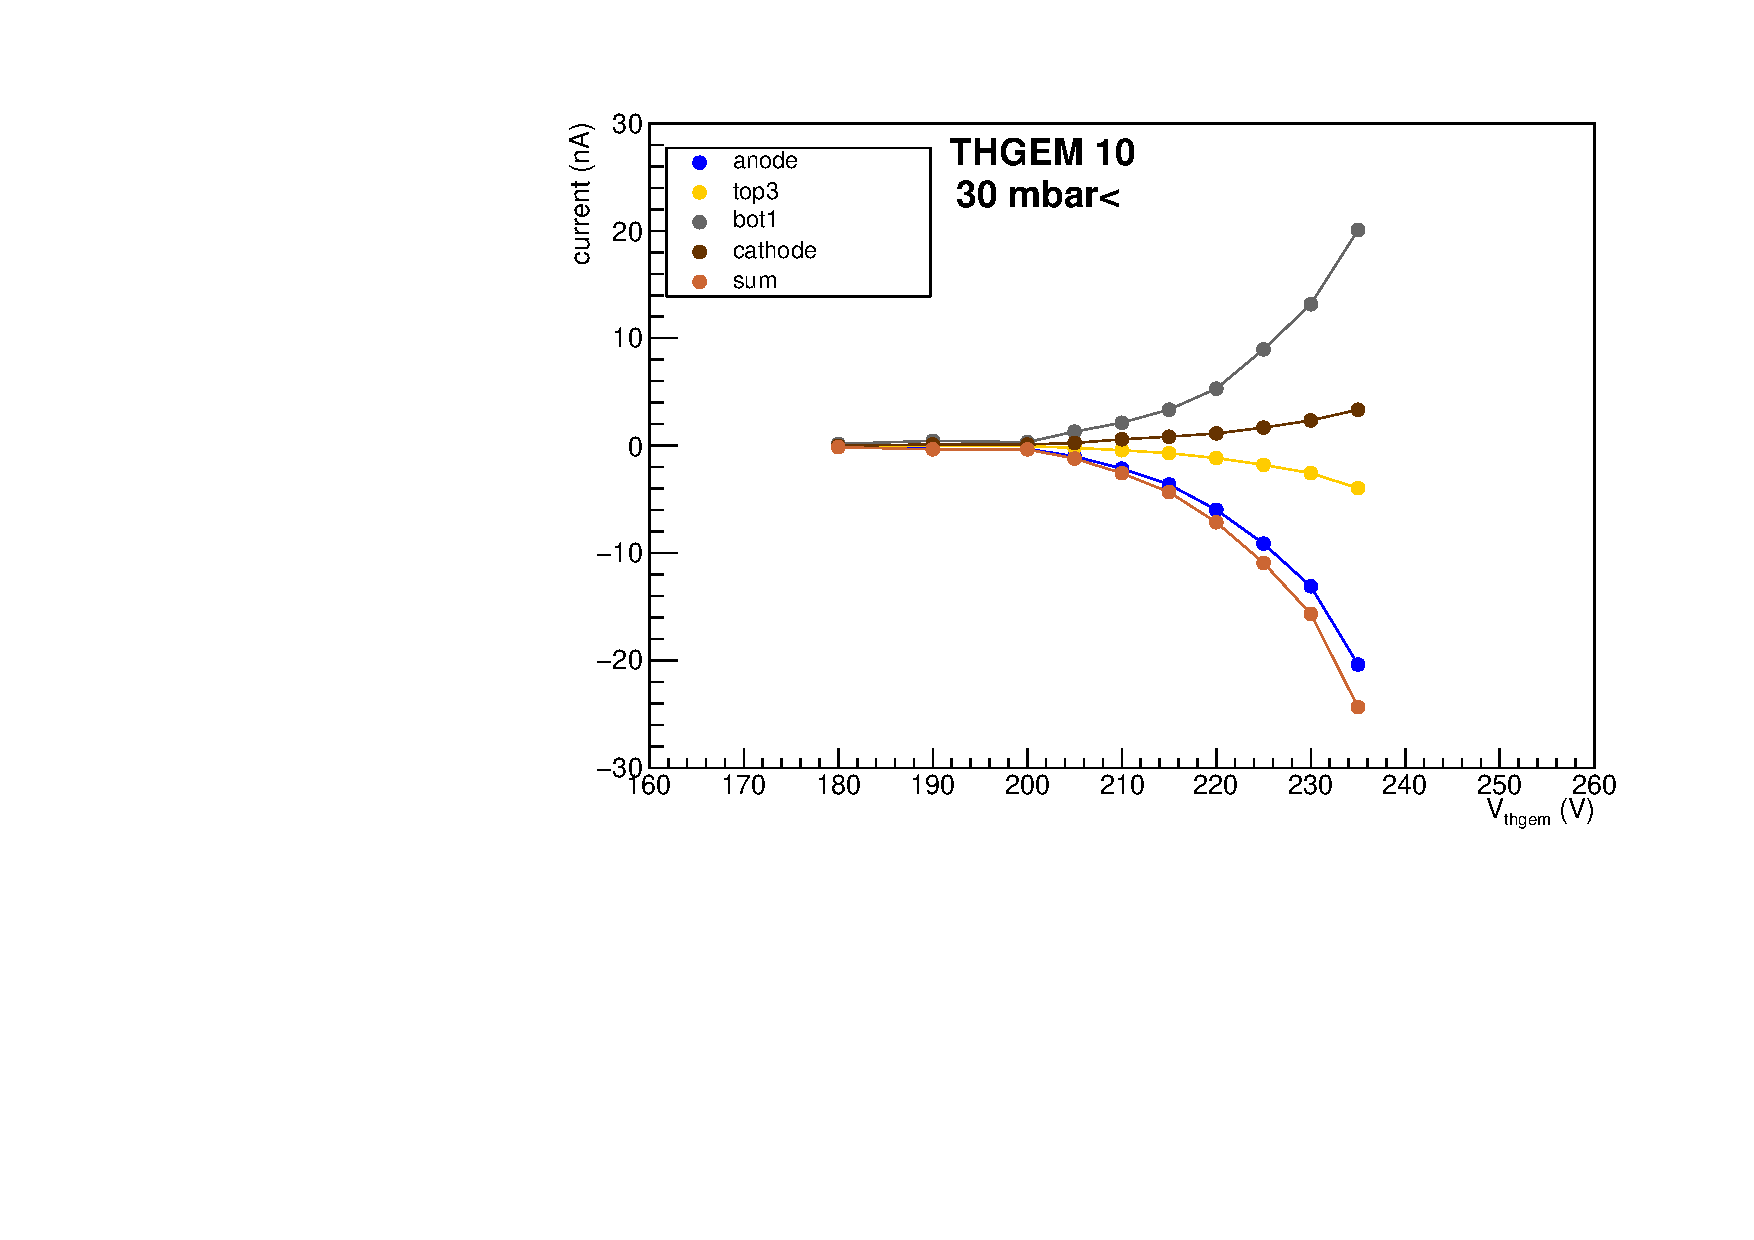
\includegraphics[width=\textwidth]{Immagini/thgemScan_THGEM10_30mbar.pdf}
	\caption{Currents measured during the scan on the voltage \Vthgem{} across each FULL THGEM at 30~mbar.}
	\label{fig:thgem_FULLTHGEM_30mbar}
\end{figure}

%%% DOPO AGGIUNTA NUOVI RUN 20/02/2020
%The results for P~=~20~mbar and P~=~11~mbar are respectively shown in Figure~\ref{fig:thgem_FULLTHGEM_20mbar} and~\ref{fig:thgem_FULLTHGEM_10mbar}.
%In both cases, the measured currents exhibit an exponential behaviour.
%The optimal \Vthgem{} value for P~=~20~mbar is 205~V, while for P~=~11~mbar it is 190~V.
%The results for P~=~20~mbar are shown in Figure~\ref{fig:thgem_FULLTHGEM_20mbar}, while those for P~=~11~mbar and P~=~9.3~mbar are respectively shown in Figure~\ref{fig:thgem_FULLTHGEM_10mbar} and~\ref{fig:thgem_FULLTHGEM_10mbar_bis}.
%In the three cases, the measured currents exhibit an exponential behaviour.
%The optimal \Vthgem{} value for P~=~20~mbar is 205~V, while for P~=~11~mbar and P~=~9.3~mbar it is 190~V.
%The results for P~=~20~mbar are shown in Figure~\ref{fig:thgem_FULLTHGEM_20mbar}: also in this case the measured currents exhibit an exponential behaviour.
%The optimal \Vthgem{} value for P~=~20~mbar is 205~V.
%
%The results for P~=~11 and~9.3~mbar are respectively shown in Figure~\ref{fig:thgem_FULLTHGEM_10mbar} and~\ref{fig:thgem_FULLTHGEM_10mbar_bis}.
%In this cases, the optimal \Vthgem{} value is 190~V.
%

%The test with P~=~9.3~mbar will be compared to another one conducted in the same conditions of pressure, \Vind{} and \Vdrift, but with an heavy ion beam instead of the $\alpha$~source (see Section~\ref{sec:test_beam}).

%\begin{figure}[htbp]
%	\centering
%	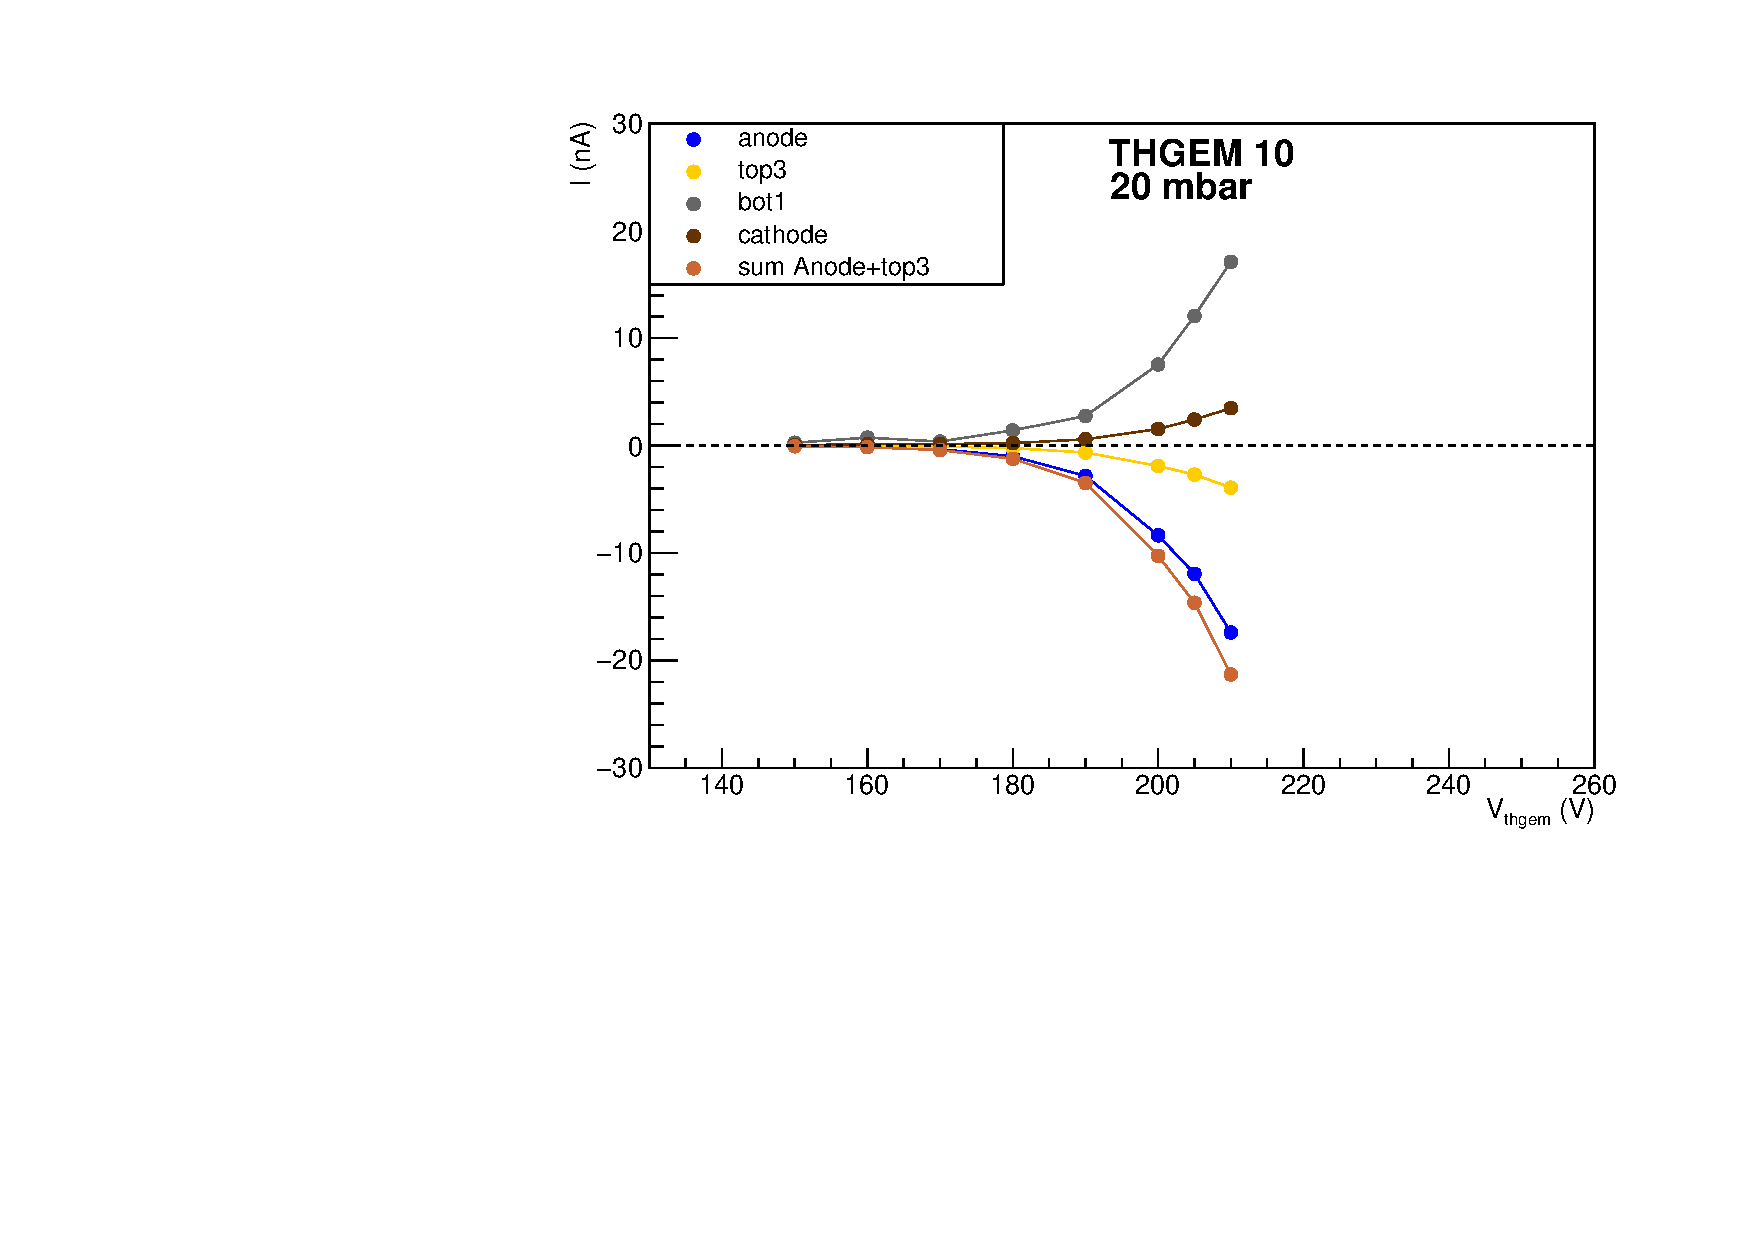
\includegraphics[width=\textwidth]{Immagini/thgemScan_THGEM10_20mbar.pdf}
%	\caption{Currents measured during the scan on the voltage \Vthgem{} across each FULL THGEM at 20~mbar, fixing \Vind~=~100~V and \Vdrift~=~1000~V.}
%	\label{fig:thgem_FULLTHGEM_20mbar}
%\end{figure}

\begin{figure}[!htb]
	\centering
	\subfigure[]{ \label{fig:thgem_FULLTHGEM_20mbar} 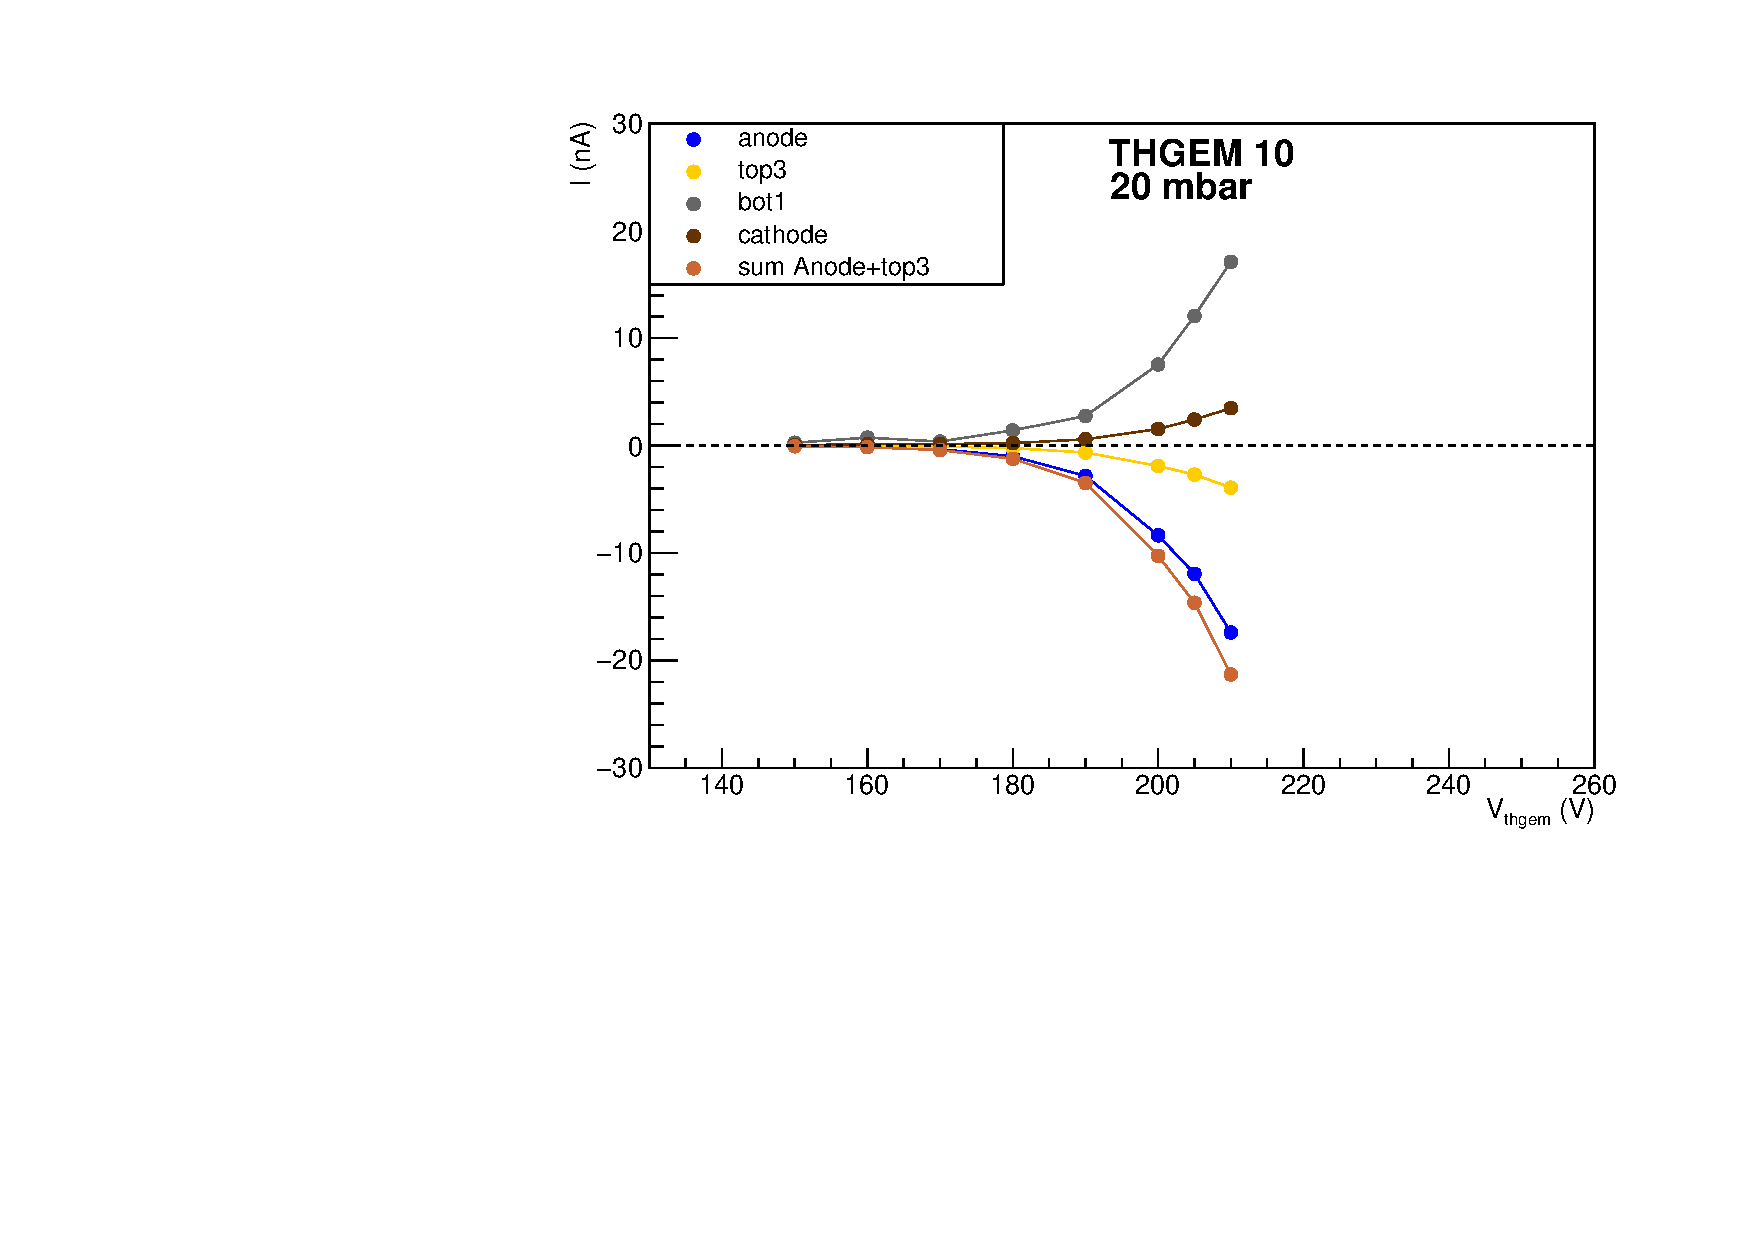
\includegraphics[width=0.96\textwidth]{Immagini/thgemScan_THGEM10_20mbar.pdf}}
	\subfigure[]{ 	\label{fig:thgem_FULLTHGEM_10mbar} 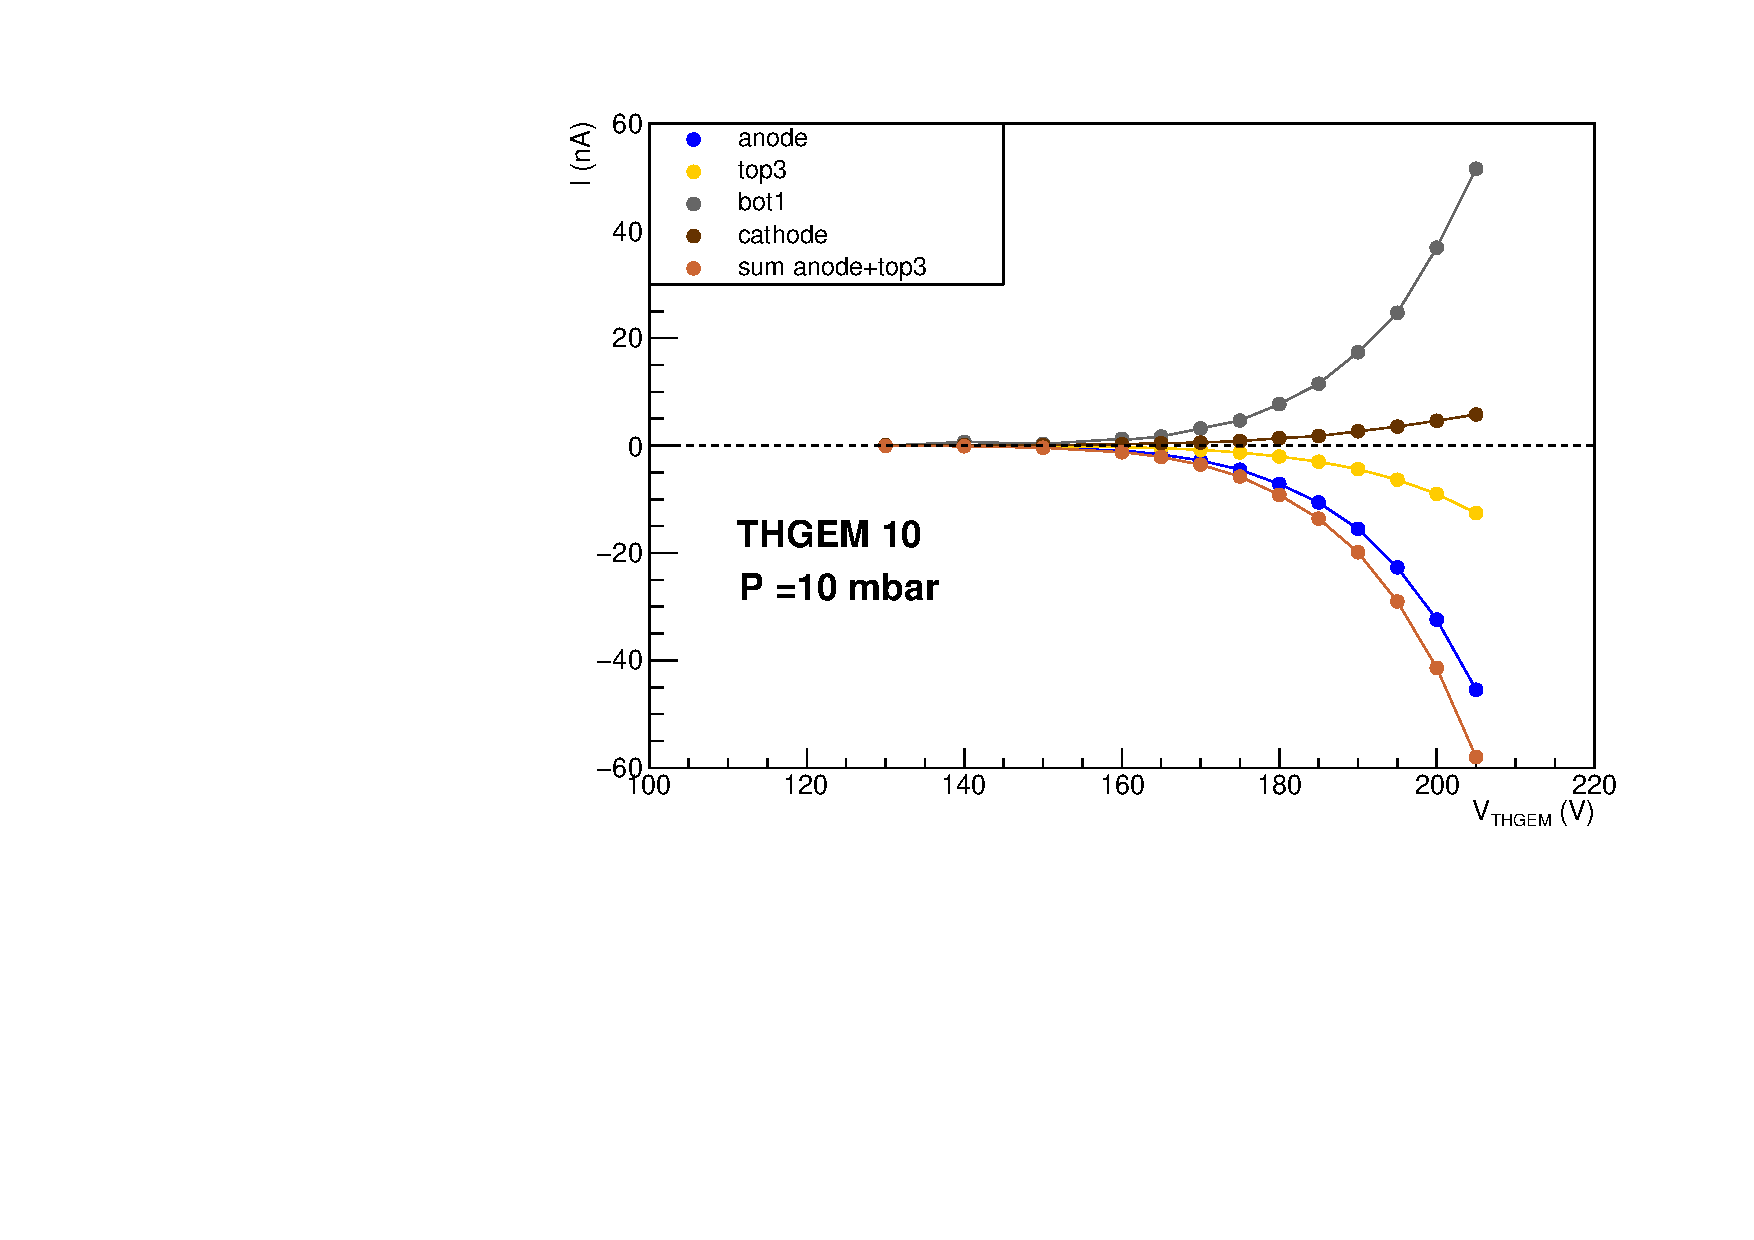
\includegraphics[width=0.96\textwidth]{Immagini/thgemScan_THGEM10_10mbar.pdf}}
	\caption{Currents measured during the scan on the voltage \Vthgem{} across each FULL THGEM: in (a) with P~=~20~mbar, \Vind~=~100~V and \Vdrift~=~1000~V, in (b) with P~=~11~mbar, \Vind~=~70~V and \Vdrift~=~600~V.}
	\label{fig:thgem_FULLTHGEM_20and10mbar}
\end{figure}

%\textcolor{red}{Aggiungere qui il discorso sul fattore di moltiplicazione?}

From these measurements, the multiplication factors (MFs) were evaluated as a function of \Vthgem{} and pressure.
The results of the calculations are shown in Figure~\ref{fig:multiplication_factor_FULL}: in the three cases the growth of the electron number in the avalanche follows with good approximation an exponential behaviour.
For a fixed value of \Vthgem, the MF decreases with increasing the pressure.
This is clearly understood, because when the pressure increases the reduced electric field decreases.
{\it explain how the multiplication factor have been calculated!!!}

\begin{figure}[!t]
	\centering
	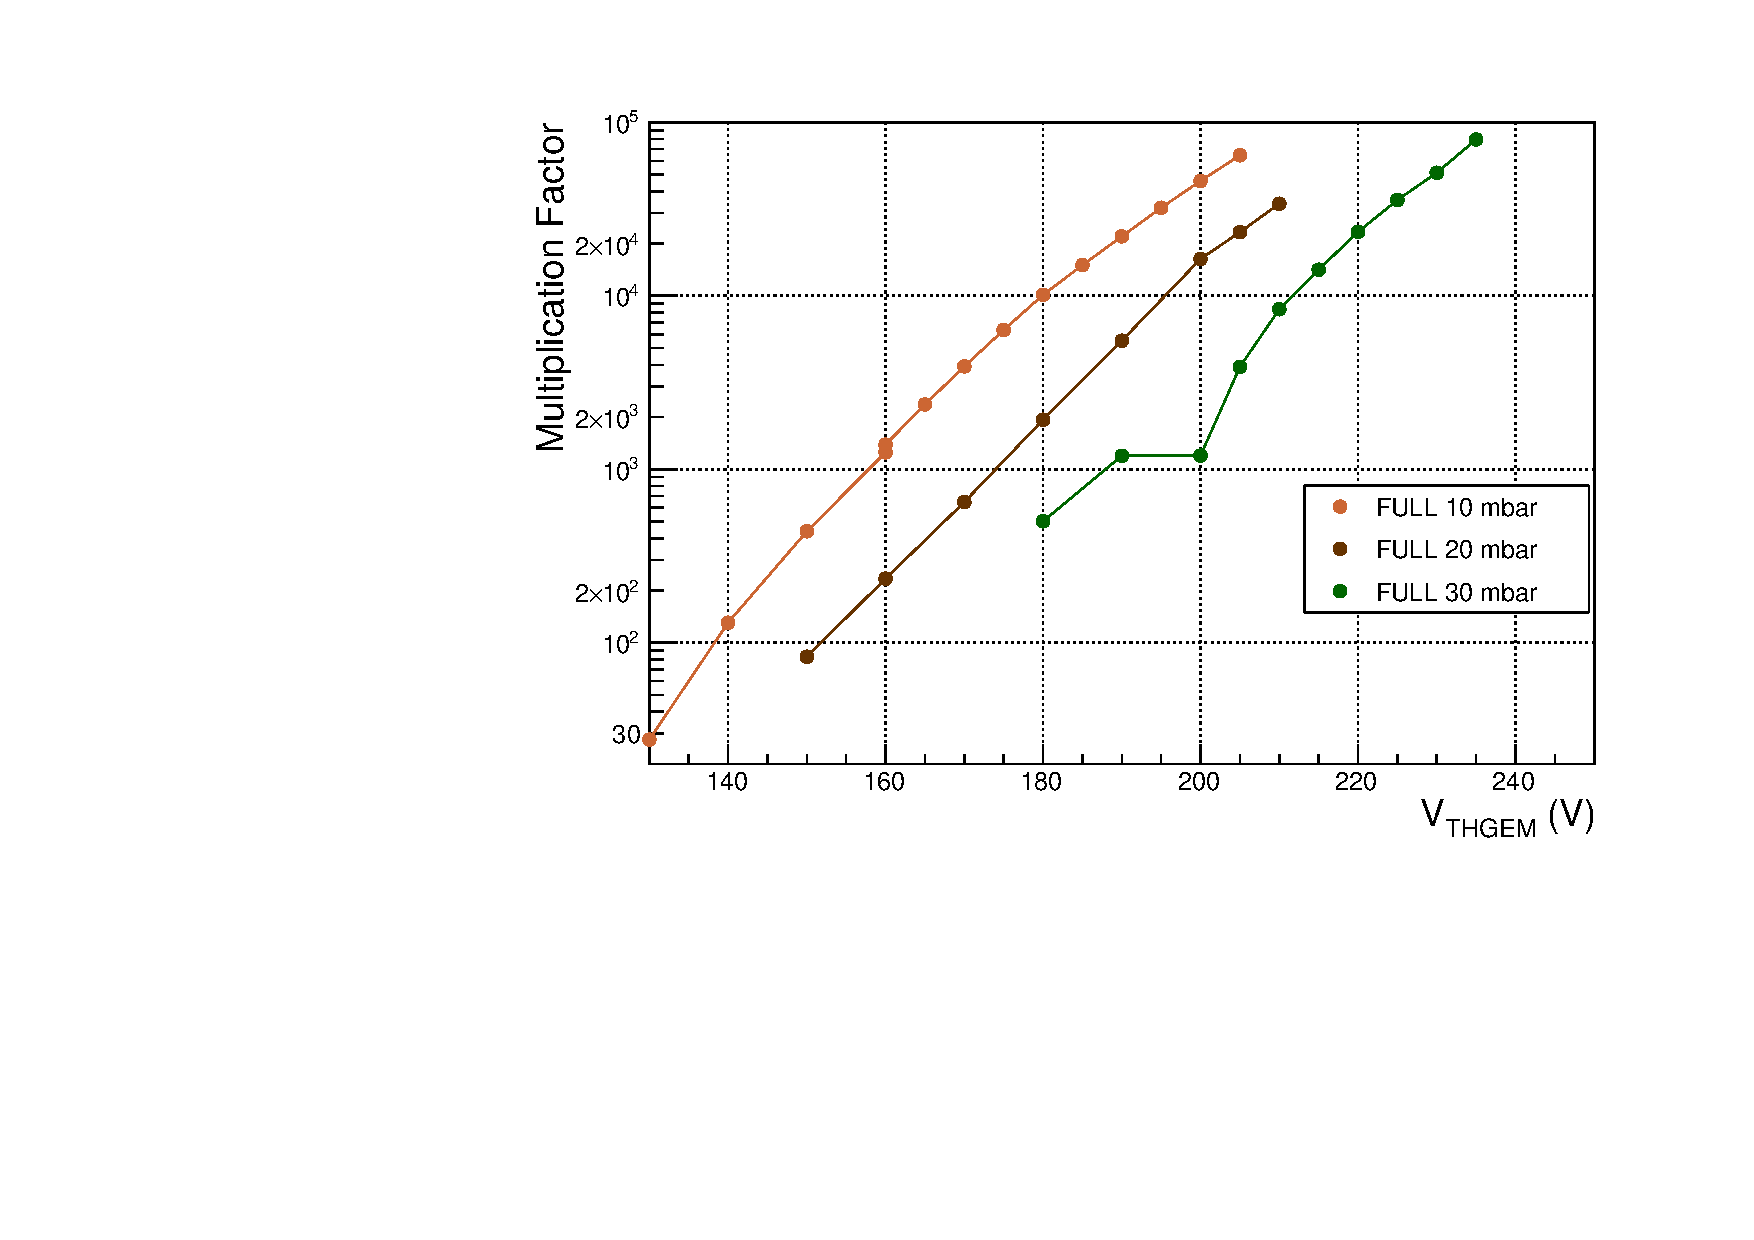
\includegraphics[width=\textwidth]{Immagini/MFvsTHGEM_FULL.pdf}
	\caption{The multiplication factors evaluated for the FULL THGEM as a function of \Vthgem{} and pressure.}
	\label{fig:multiplication_factor_FULL}
\end{figure}




%\subsubsection*{Scan on THGEM voltage  at 30 mbar}
%To find the optimal value for the THGEM voltage until discharge, a scan on this parameter has been done. The measured currents obtained for a pressure of 30~mbar and for \Vind~=~120~V and \Vdrift~=~1000~V are shown in Figure~\ref{fig:thgem_FULLTHGEM_30mbar}. \Vthgem~=~180~V is the minimum voltage at which anode current is measurable. At \Vthgem~=~230~V there was discharges, but we do not know if it came from THGEM. The anode current has the typical exponential behaviour.

\clearpage

\subsubsection{Scan on \Vdrift}

To fully characterize the tracker response, a study was conducted varying the potential difference \Vdrift{} across the drift region, while pressure, \Vind{} and \Vthgem{} were kept fixed.
The explored range goes from 0~V (or 100~V in the case with P~=~20~mbar) to the discharge voltage, which depends on the gas pressure: for P~=~30~mbar it was 1600~V, for P~=~20~mbar it was 1200~V, and for P~=~11~mbar it was 800~V.
The increments were of 50~V for P~=~11~mbar, while in the other two cases it was of 100~V.
In Table~\ref{tab:FULLTHGEM_vdrift} the adopted value of pressure, \Vind{} and \Vthgem{} are shown.

\begin{table} [!h]
	\begin{center}
		\renewcommand{\arraystretch}{1.2}
		\begin{tabular} {ccccc}
			P (mbar) & & \Vind{} (V) & & \Vthgem{} (V)\\
			\toprule[0.1em]
			%\hline
			30	& &	120	& &	220 \\
			20	& &	100	& & 205 \\
			11	& & 70	& & 190 \\
			11	& & 70	& & 170 \\
			
			\bottomrule[0.1em]
		\end{tabular}
	\end{center}
	\caption{The values of pressure (P), \Vind{} and \Vthgem{} adopted for the study on \Vdrift.} \label{tab:FULLTHGEM_vdrift}
\end{table}

The result of the scan at 30~mbar is displayed in Figure~\ref{fig:drift_FULLTHGEM_30mbar}. 
All the measured currents are saturated at 100~V.
In order to better understand the THGEM response at low drift voltage, further measurements were done with \Vdrift~=~5~V, 10~V, 20~V, and 30~V.
The result of this measurement, shown in Figure~\textcolor{red}{aggiungere la figura zoomata}, is that currents are saturated already at 5~V.
This means that either the magnitude of the electric field at \Vdrift~=~0~V is much lower than $5/20\; \mbox{(V/cm)}= 250 \; \mbox{(mV/cm)}$ or the value measured by PICO actually is not zero.
\begin{figure}[htbp]
	\centering
	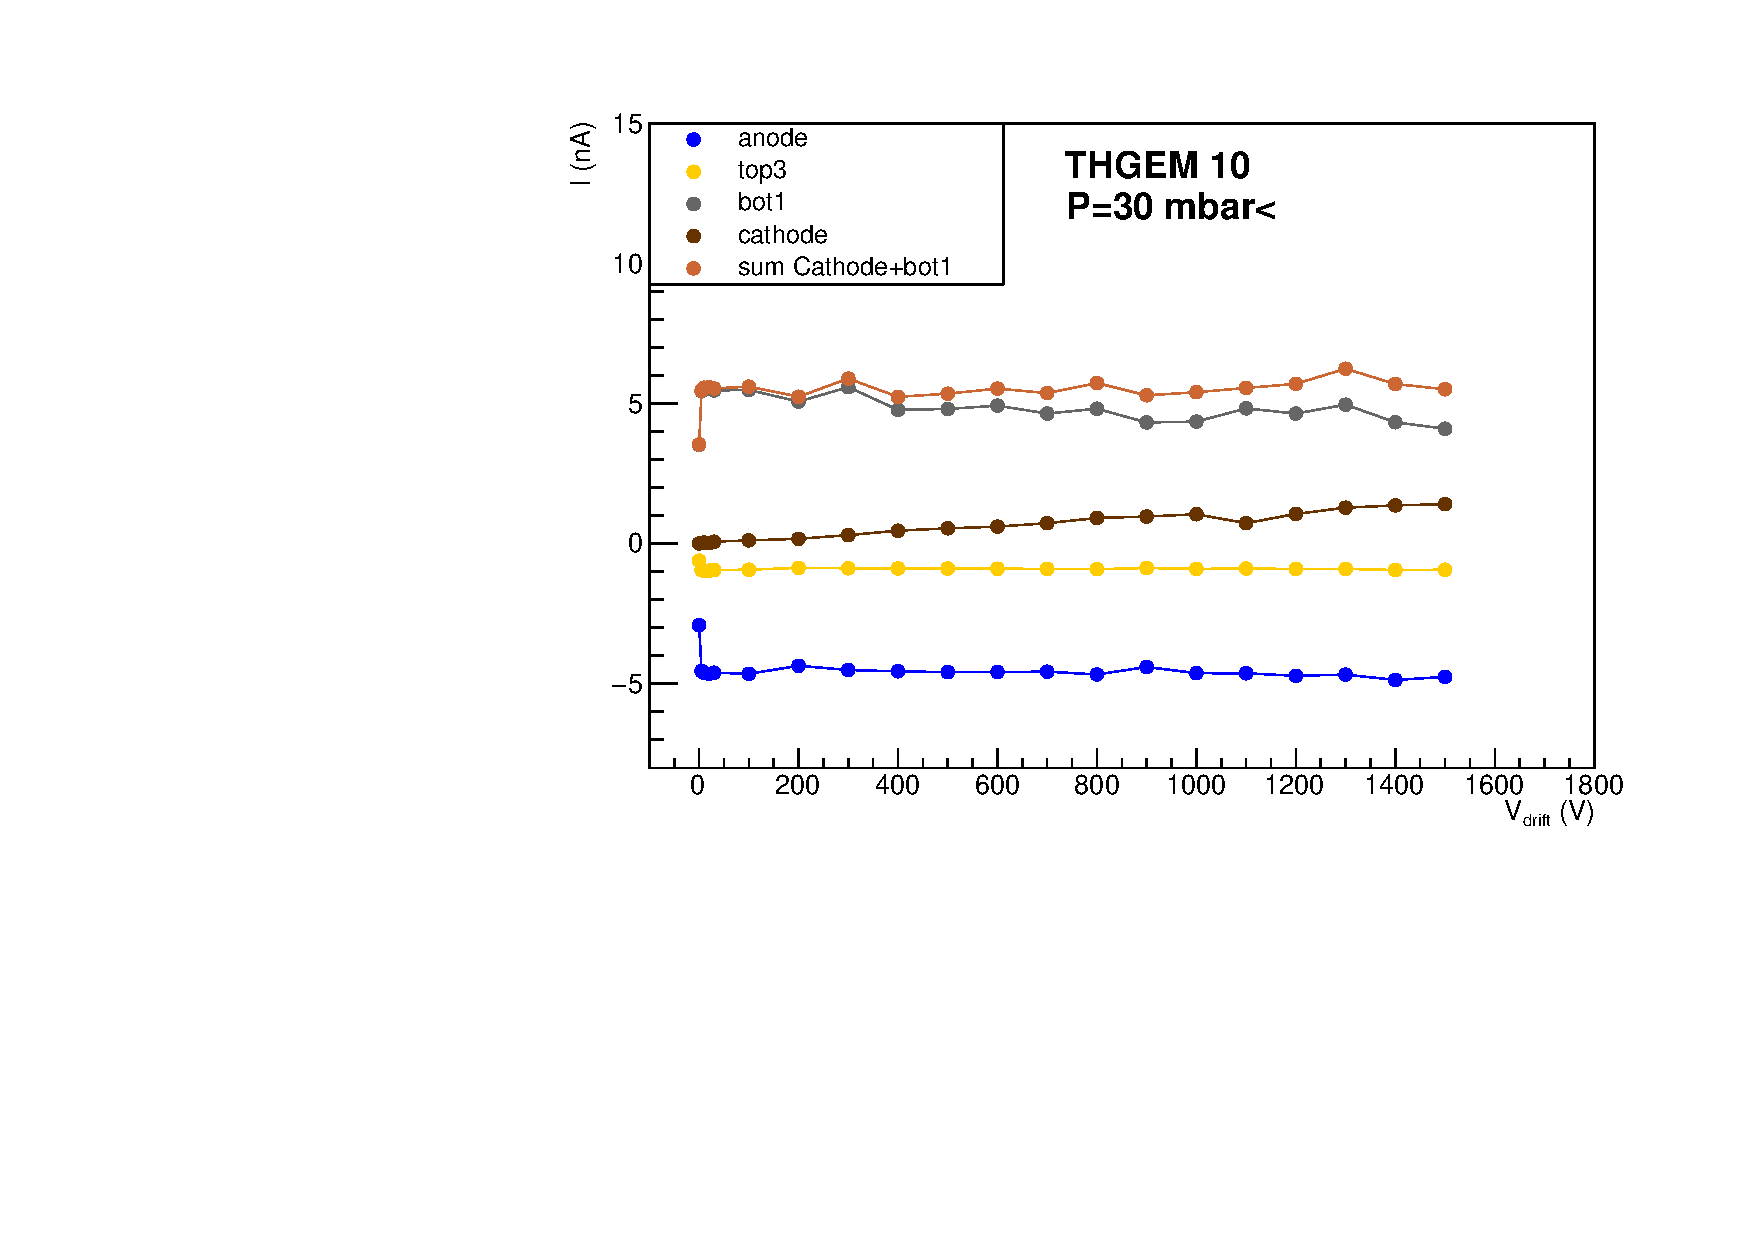
\includegraphics[width=\textwidth]{Immagini/driftScan_THGEM10_30mbar.pdf}
	\caption{Currents measured during the scan on the voltage \Vdrift{} across the drift region at 30~mbar.}
	\label{fig:drift_FULLTHGEM_30mbar}
\end{figure}

In Figure~\ref{fig:drift_FULLTHGEM_30mbar} the orange line represents, in this case, the sum of the cathode and bot1 currents.
This quantity is important to estimate the ion backflow. 
%\textcolor{red}{Aggiungere spiegazione ion backflow}.
%\textcolor{red}{Fare un grafico con l'ion backflow o inserire dei valori di riferimento?}



The results of the tests at 20 and 11~mbar are shown, respectively, in Figure~\ref{fig:drift_FULLTHGEM_20mbar} and~\ref{fig:drift_FULLTHGEM_11mbar}.
Also in these cases the saturation voltage is 100~V.



\begin{figure}[!htb]
	\centering
	\subfigure[]{ \label{fig:drift_FULLTHGEM_20mbar} 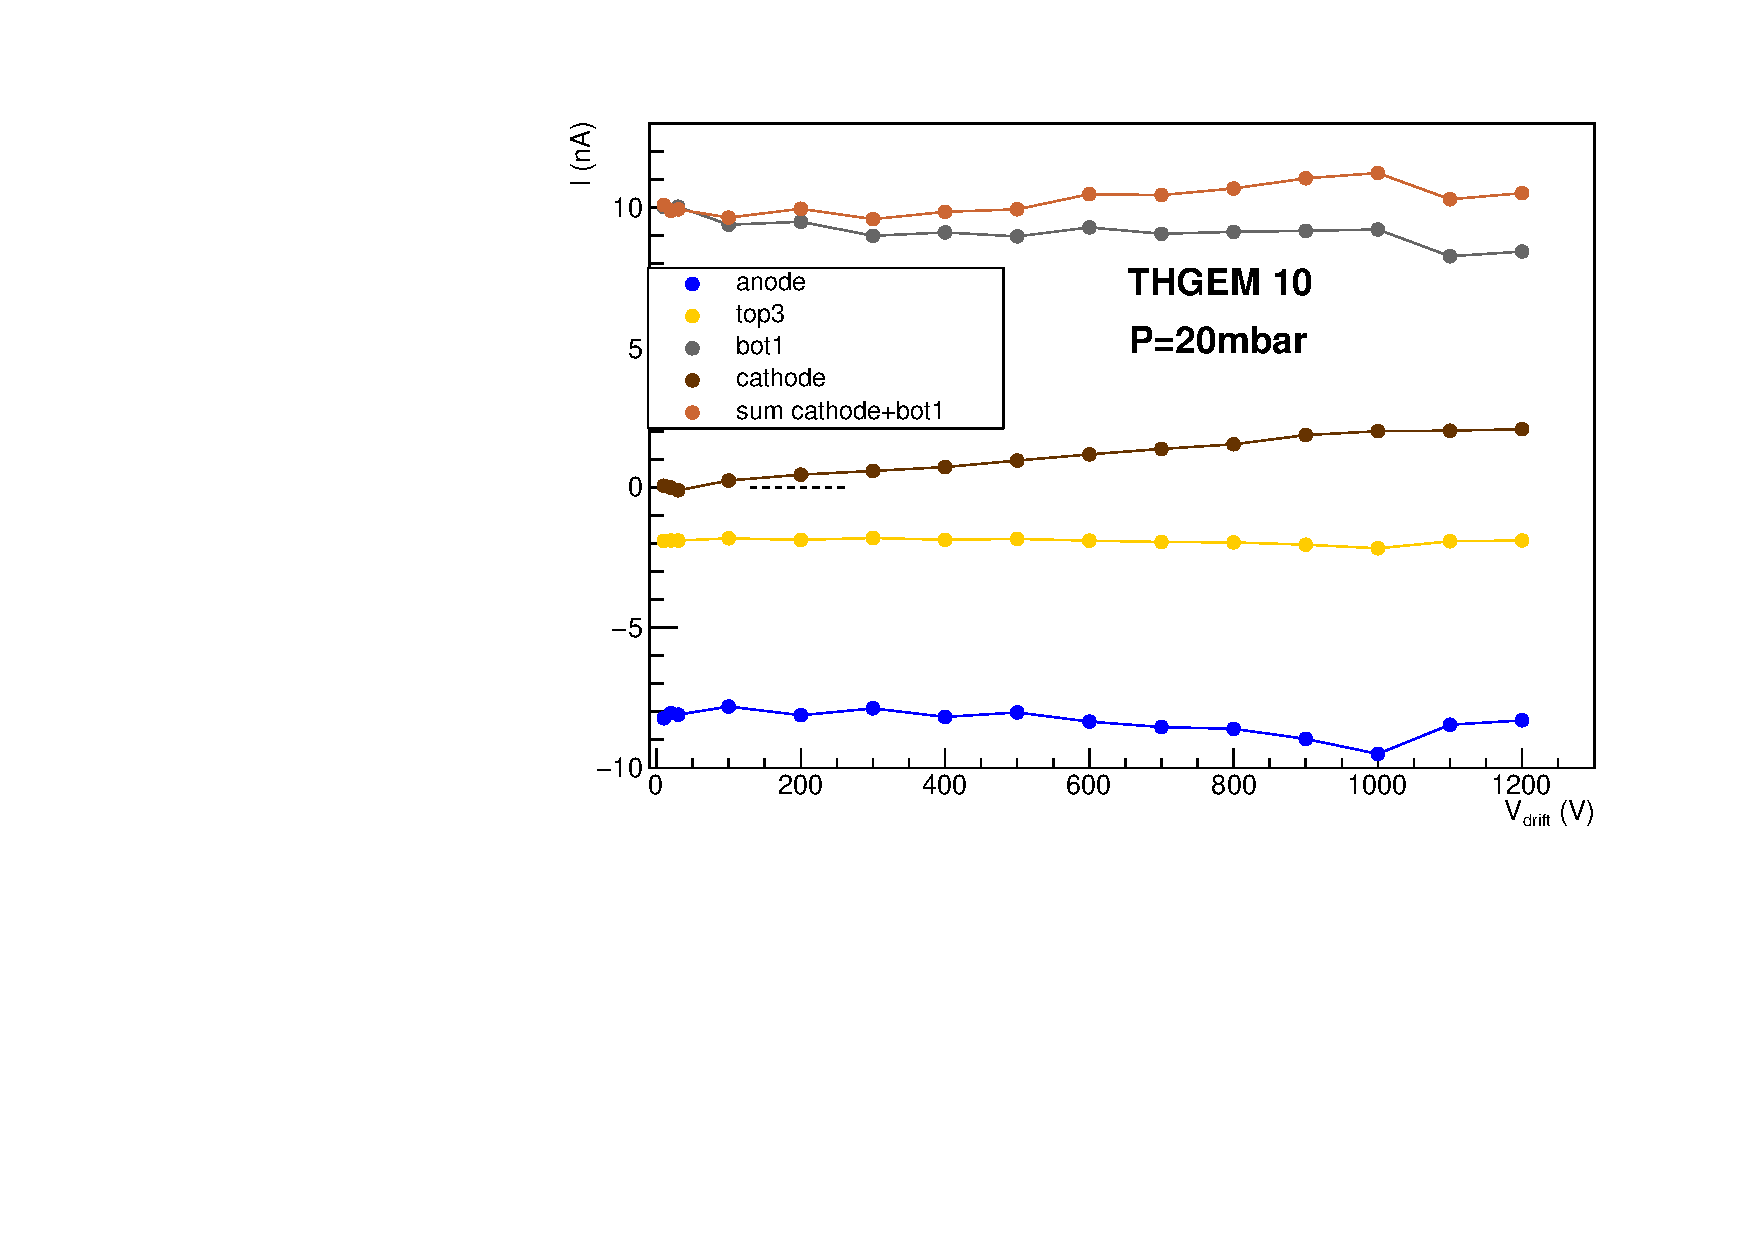
\includegraphics[width=0.96\textwidth]{Immagini/driftScan_THGEM10_20mbar.pdf}}
	\subfigure[]{ 	\label{fig:drift_FULLTHGEM_11mbar} 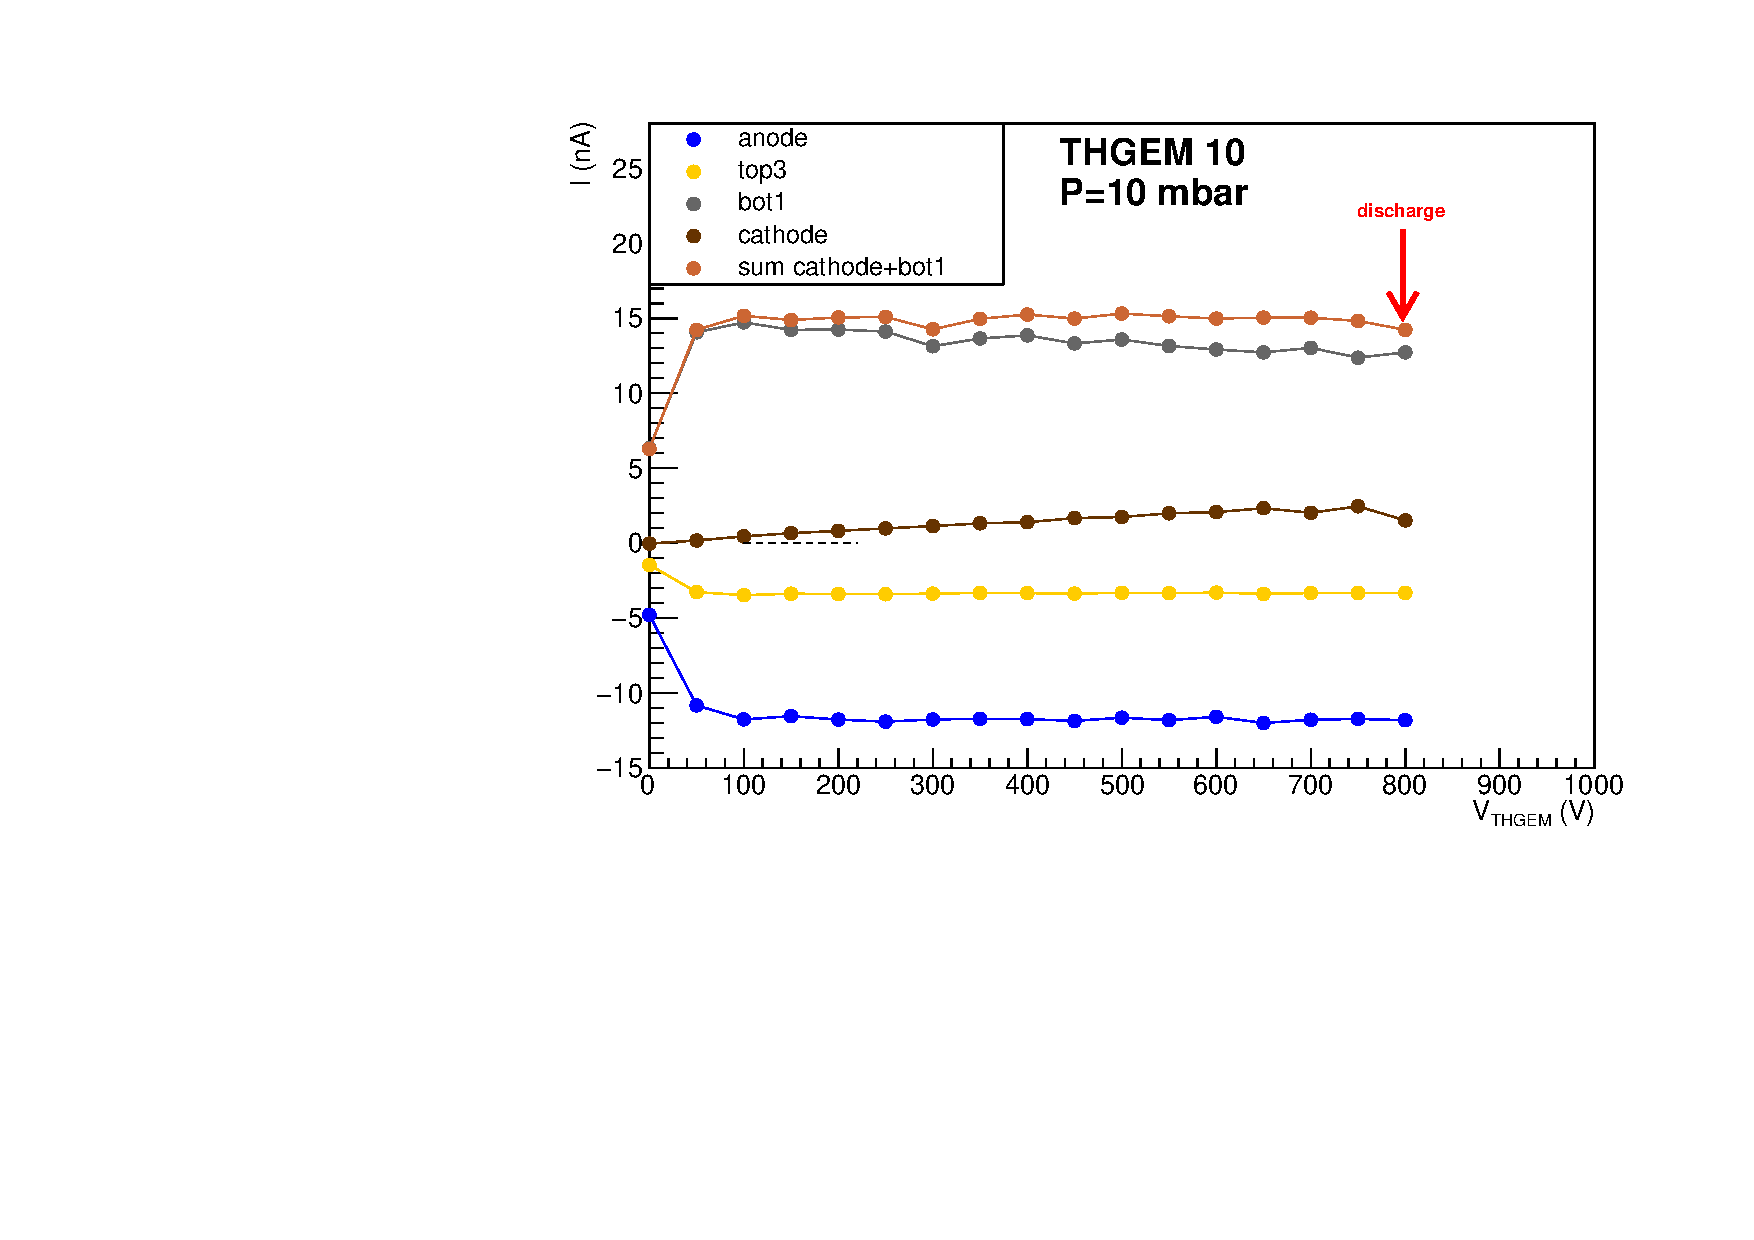
\includegraphics[width=0.96\textwidth]{Immagini/driftScan_THGEM10_10mbar.pdf}}
	\caption{Currents measured during the scan on the voltage \Vdrift{} across the drift region: in (a) at 20~mbar, in (b) at 11~mbar.}
	\label{fig:drift_FULLTHGEM_other_pressure}
\end{figure}



%\textcolor{red}{Aggiungere plot sul backflow}
From these measurements, the ion backflow of the FULL THGEM was evaluated as a function of \Vdrift{} and pressure.
The results of the calculation are shown in Figure~\ref{fig:ion_backflow_FULL}: the ion backflow linearly increases at increasing \Vdrift{} and is approximately independent from pressure.

\begin{figure}[htbp]
	\centering
	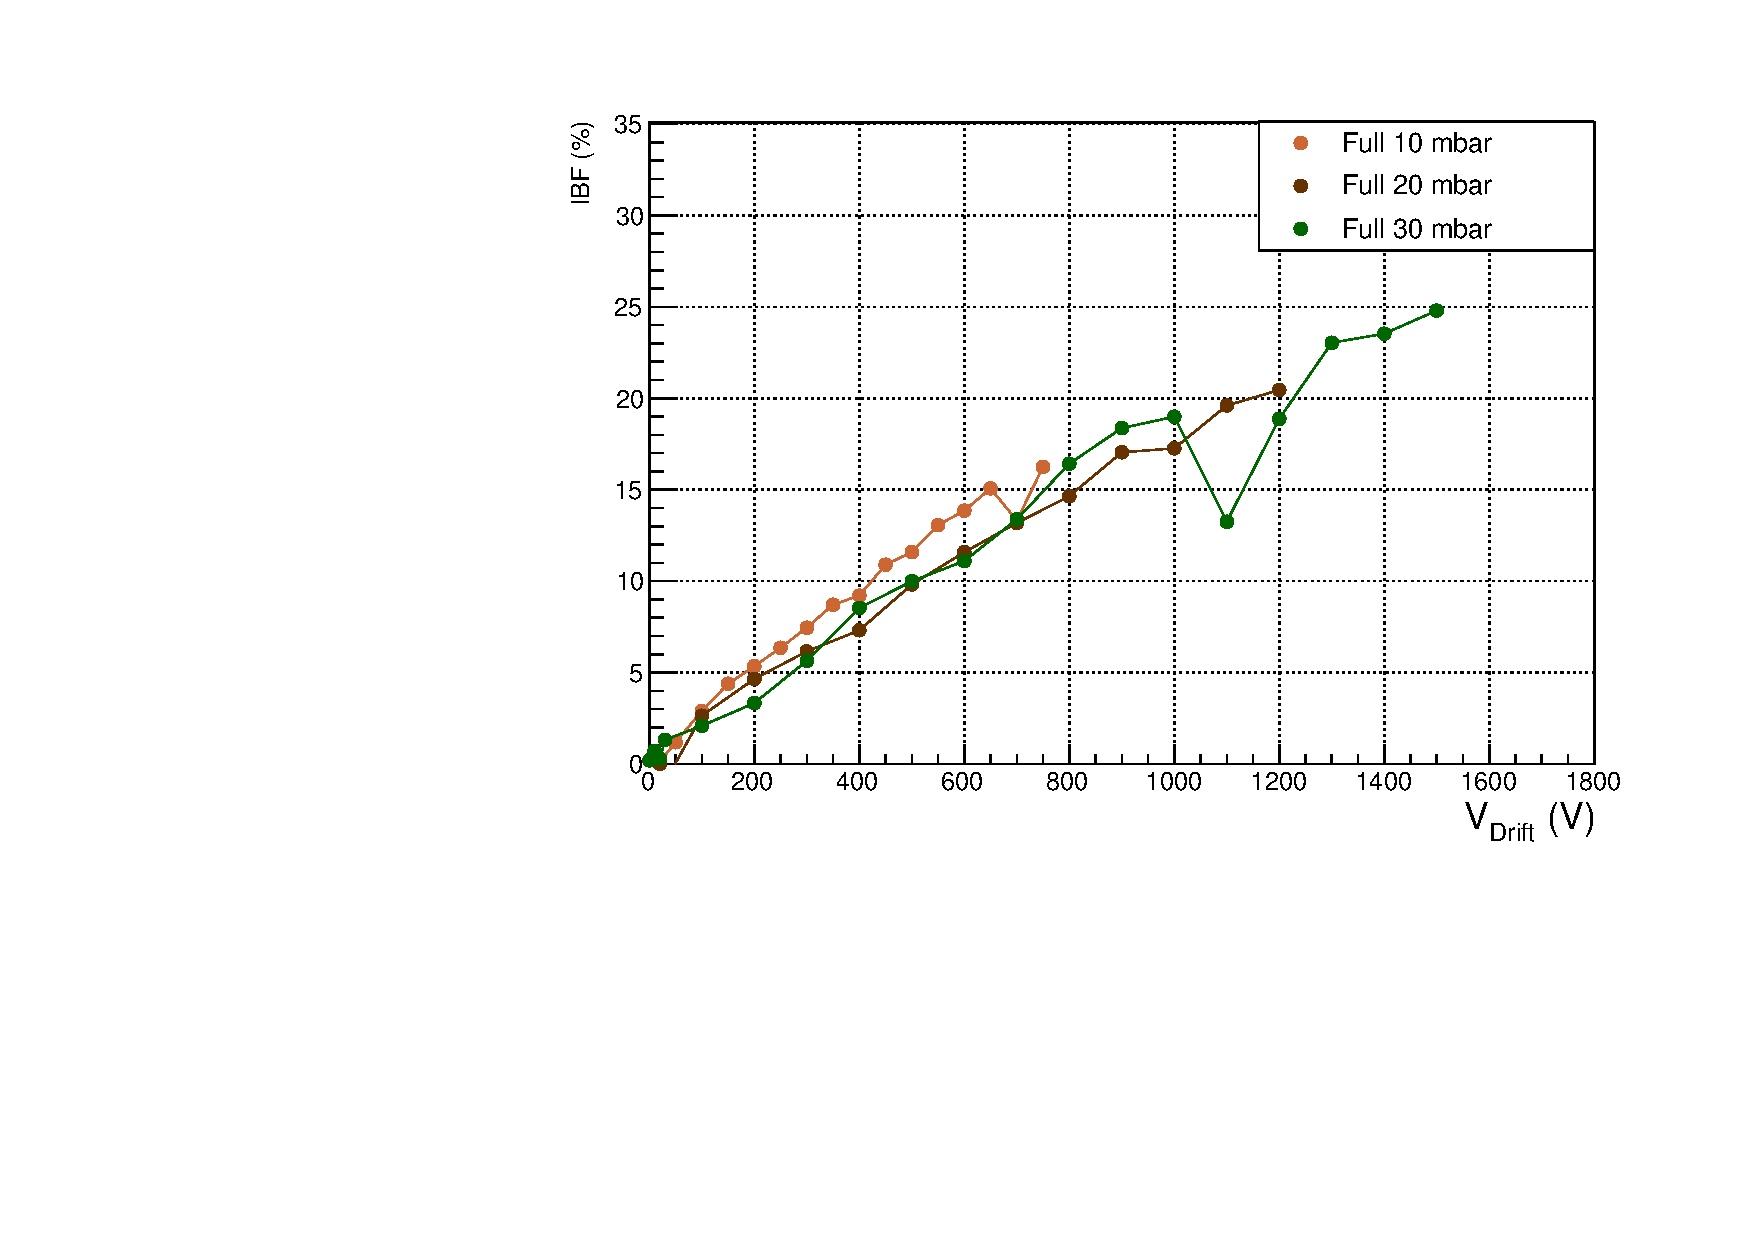
\includegraphics[width=\textwidth]{Immagini/IBFvsDrift_FULLonly.pdf}
	\caption{The ion backflow as a function of \Vdrift{} for the three examined pressures.}
	\label{fig:ion_backflow_FULL}
\end{figure}



%\subsubsection*{Scan on drift voltage  at 30 mbar}
%To find the optimal value for the drift voltage until discharge, a scan on this parameter has been done. The measured currents obtained for a pressure of 30~mbar and for \Vind~=~120~V and \Vthgem~=~220~V are shown in Figure~\ref{fig:drift_FULLTHGEM_30mbar}. At \Vdrift~=~5~V the anodic current is saturated. This means that the magnitude of the electric field at \Vdrift~=~0~V is much lower than $\frac{5~V}{20~cm}= 250 mV/cm$ or the value measured by PICO is actually not zero. At \Vdrift~=~1200~V ion backflow~(\ibf) is equal to 18.9\%, while at \Vdrift~=~1500~V \ibf~is equal to 24.7\%. Dischages appeared at \Vdrift~=~1600~V.



%\subsubsection*{Scan at 20 mbar}
%The induction, THGEM and drift scan where repeated at 20~mbar and the currents curve show the same behaviour. In \Vind~scan, \Vthgem~=~200~V and \Vdrift~=~1000~V and the plateau was in the range 90$\div$120~V. The optimal value is 100~V. In \Vthgem~scan, \Vind~=~100~V and \Vdrift~=~1000~V and the last measurable signal was at 150~V. At 220~V there were discharges, so the optimal \Vthgem~value is 205~V. During \Vdrift~scan, \Vind~=~100~V and \Vthgem~=~205~V and there were discharges at 1100~V. At \Vdrift~=~700~V, the estimated value of \ibf is 13.2\%, whilst at \Vdrift~=~1000~V  \ibf is 17.3\%.


%\subsubsection*{Scan at 10 mbar}
%The induction, THGEM and drift scan where repeated at 10~mbar and the currents curve show the same behaviour. In \Vind~scan, setting \Vthgem~=~180~V and \Vdrift~=~800~V, discharges appear at 60~V. Setting \Vthgem~=~170~V and \Vdrift~=~800~V, there were discharges mainly in bot1 and cathode currents at 60~V. So the chosen configuration is \Vthgem~=~170~V and \Vdrift~=~600~V. In this way, no discharges were visible.The highest \Vind~value explored was 150~V. Also for this pressure, a plateau was found in the range 60$\div$80~V. The optimal value is 70~V. In \Vthgem~scan, \Vind~=~70~V and \Vdrift~=~600~V and the last measurable signal was at 130~V. At 210~V there were discharges, so the optimal \Vthgem~value is 190~V. During \Vdrift~scan, \Vind~=~70~V and \Vthgem~=~190~V and there were discharges at 800~V. At \Vdrift~=~450~V, the estimated value of \ibf is 10.9\%, whilst at \Vdrift~=~750~V  \ibf is 16.2\%.

\clearpage

\subsection{ROW THGEM}
The same studies perfomed on the FULL THGEM have been repeated on the ROW THGEM.
We shortly recall the main difference between the two THGEM types \ldots

Due to the lower number of holes we expect that the currents on the ROW THGEM
are smaller compared to those of the FULL THGEM.


\subsubsection{Scan on \Vind}

%In the experimental setup employing the ROW THGEM 

%The tracker configuration employing the ROW THGEM was 

%The characterization of the ROW THGEM-based tracker 
%The ROW THGEM-based tracker 

The effects of the variation of the potential difference \Vind{} on the measured currents was studied also for the ROW THGEM-based tracker.
These measurements were done fixing three different pressure (P) and setting suitable values of \Vthgem{} and \Vdrift.
A summary scheme of the adopted configurations is shown in Table~\ref{tab:ROWTHGEM_vind}.
\begin{table} [htbp]
	\begin{center}
		\renewcommand{\arraystretch}{1.2}
		\begin{tabular} {ccccc}
			P (mbar) & & \Vthgem{} (V) & & \Vdrift{} (V)\\
			\toprule[0.1em]
			%\hline
			20	& &	220	& &	800 \\
			20	& & 210	& & 800 \\
			30	& &	240	& &	800 \\
			40	& &	260	& &	700 \\
			
			\bottomrule[0.1em]
		\end{tabular}
	\end{center}
	\caption{The values of pressure (P), \Vthgem{} and \Vdrift{} adopted for the study on \Vind.} \label{tab:ROWTHGEM_vind}
\end{table}
The \Vind{} scans were carried out starting from 0~V and increasing the voltage by 10 or 20~V per run, until the discharge value is reached.
This value is dependent on the gas pressure and on the values set for \Vthgem{} and \Vdrift: for P~=~20~mbar it was 110~V, for P~=~30~mbar it was 110~V, and for P~=~40~mbar it was 180~V.




The result of the two scans at 20~mbar are shown, respectively, in Figure~\ref{fig:induction_ROWTHGEM_20mbar} and~\ref{fig:induction_ROWTHGEM_20mbar_bis}: also with ROW THGEM it is apparent that by raising the value of \Vind{}, the anodic current (blue line) increases, while the top3 current (yellow line) approaches to zero.
%\begin{figure}[htbp]
%	\centering
%	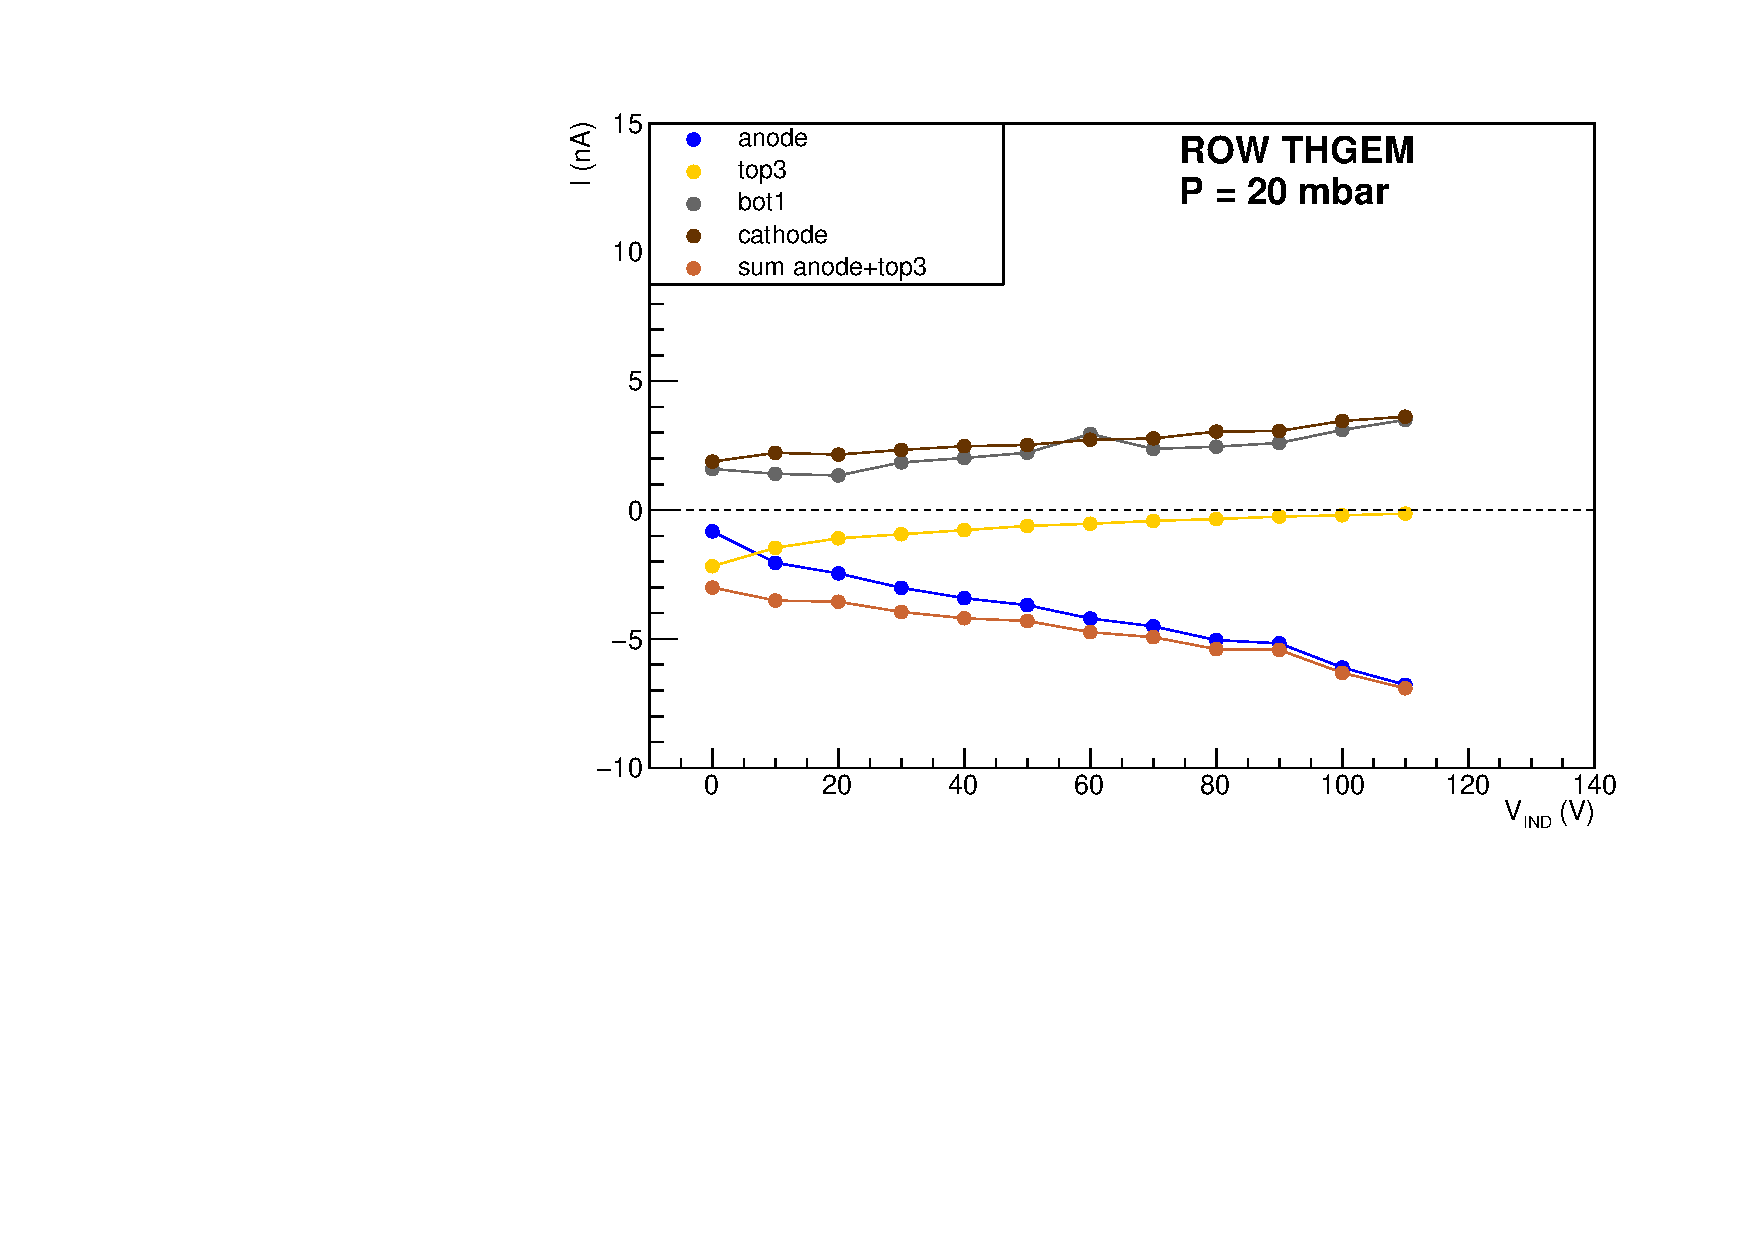
\includegraphics[width=\textwidth]{Immagini/InductionScan_ROW_THGEM_20mbar.pdf}
%	\caption{Currents measured during the scan on the voltage \Vind{} across the induction region at 30~mbar and with \Vthgem{}~=~220~V.}
%	\label{fig:induction_ROWTHGEM_20mbar}
%\end{figure}
\begin{figure}[!htb]
	\centering
	\subfigure[]{ \label{fig:induction_ROWTHGEM_20mbar} 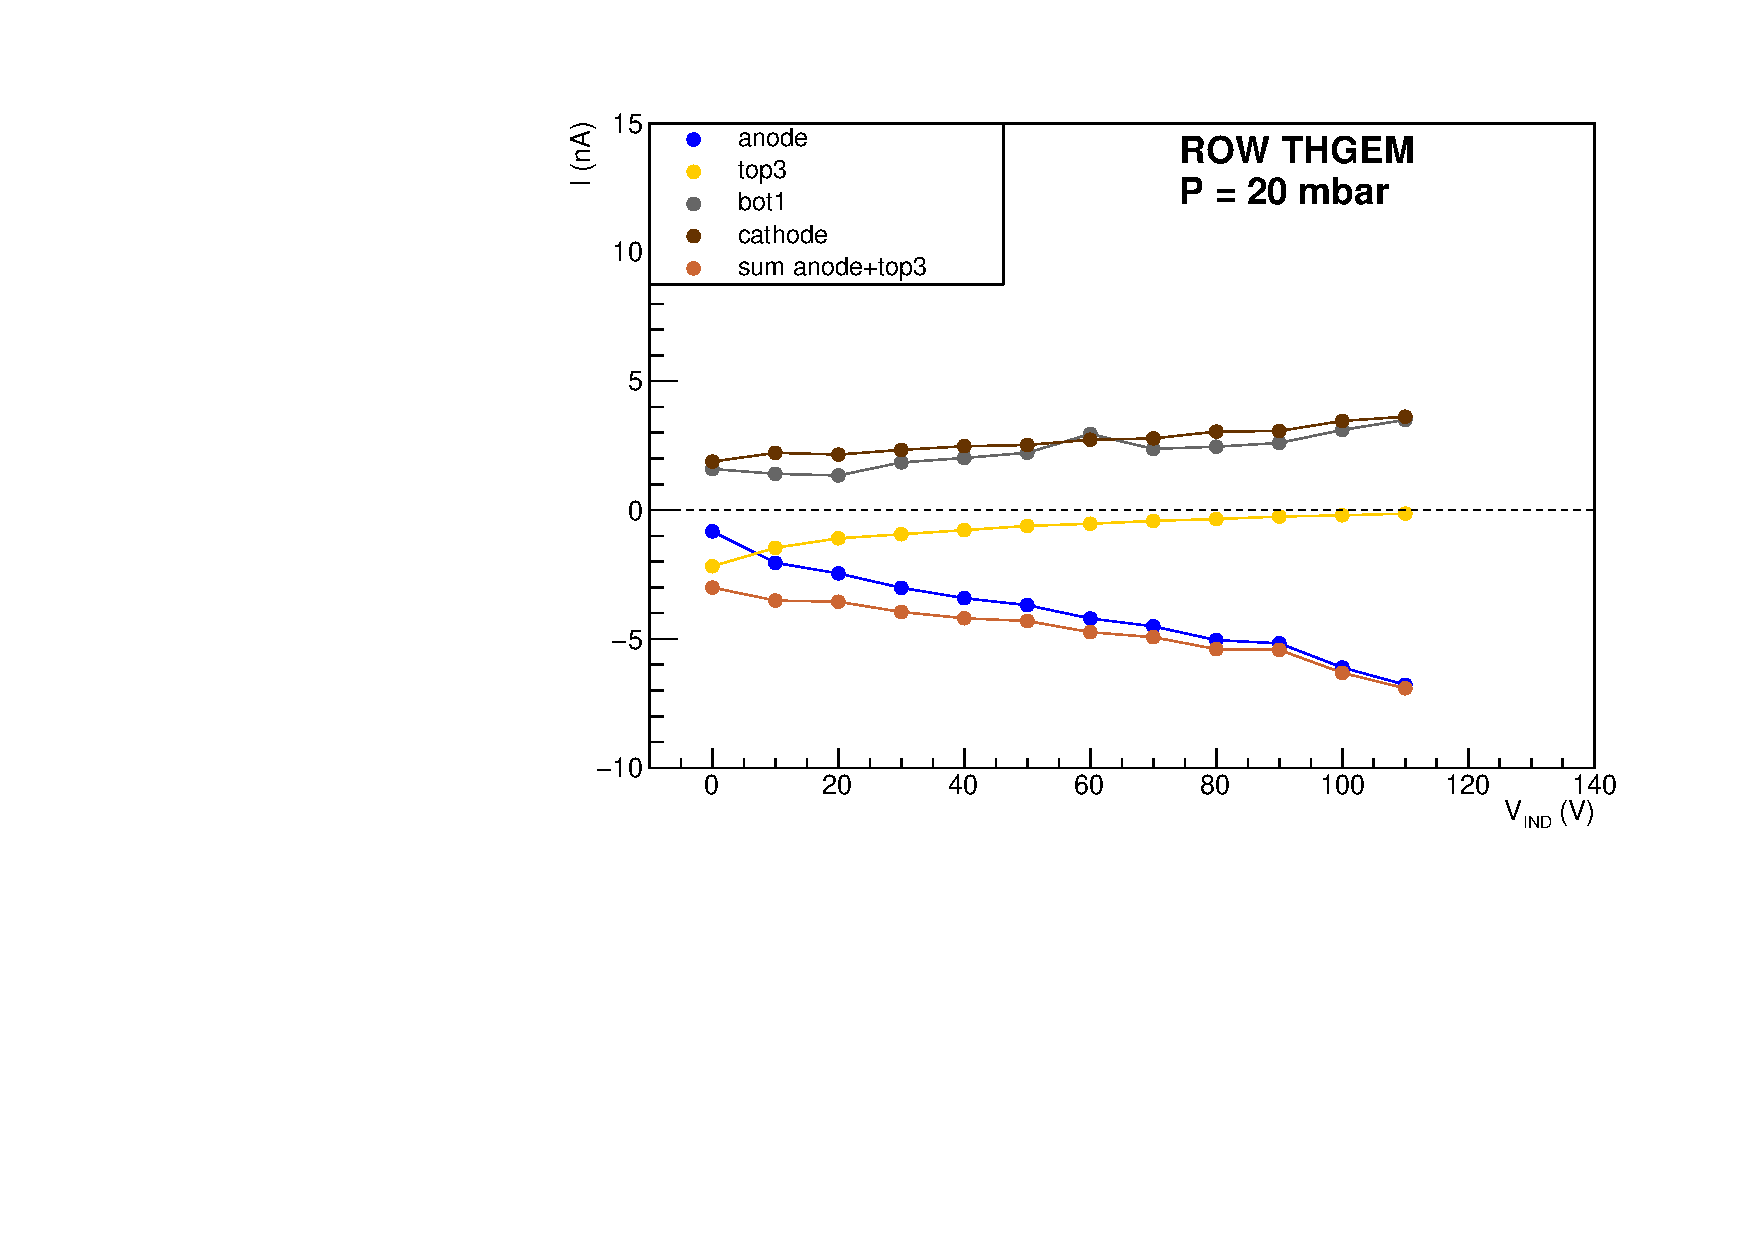
\includegraphics[width=0.96\textwidth]{Immagini/InductionScan_ROW_THGEM_20mbar.pdf}}
	\subfigure[]{ 	\label{fig:induction_ROWTHGEM_20mbar_bis} 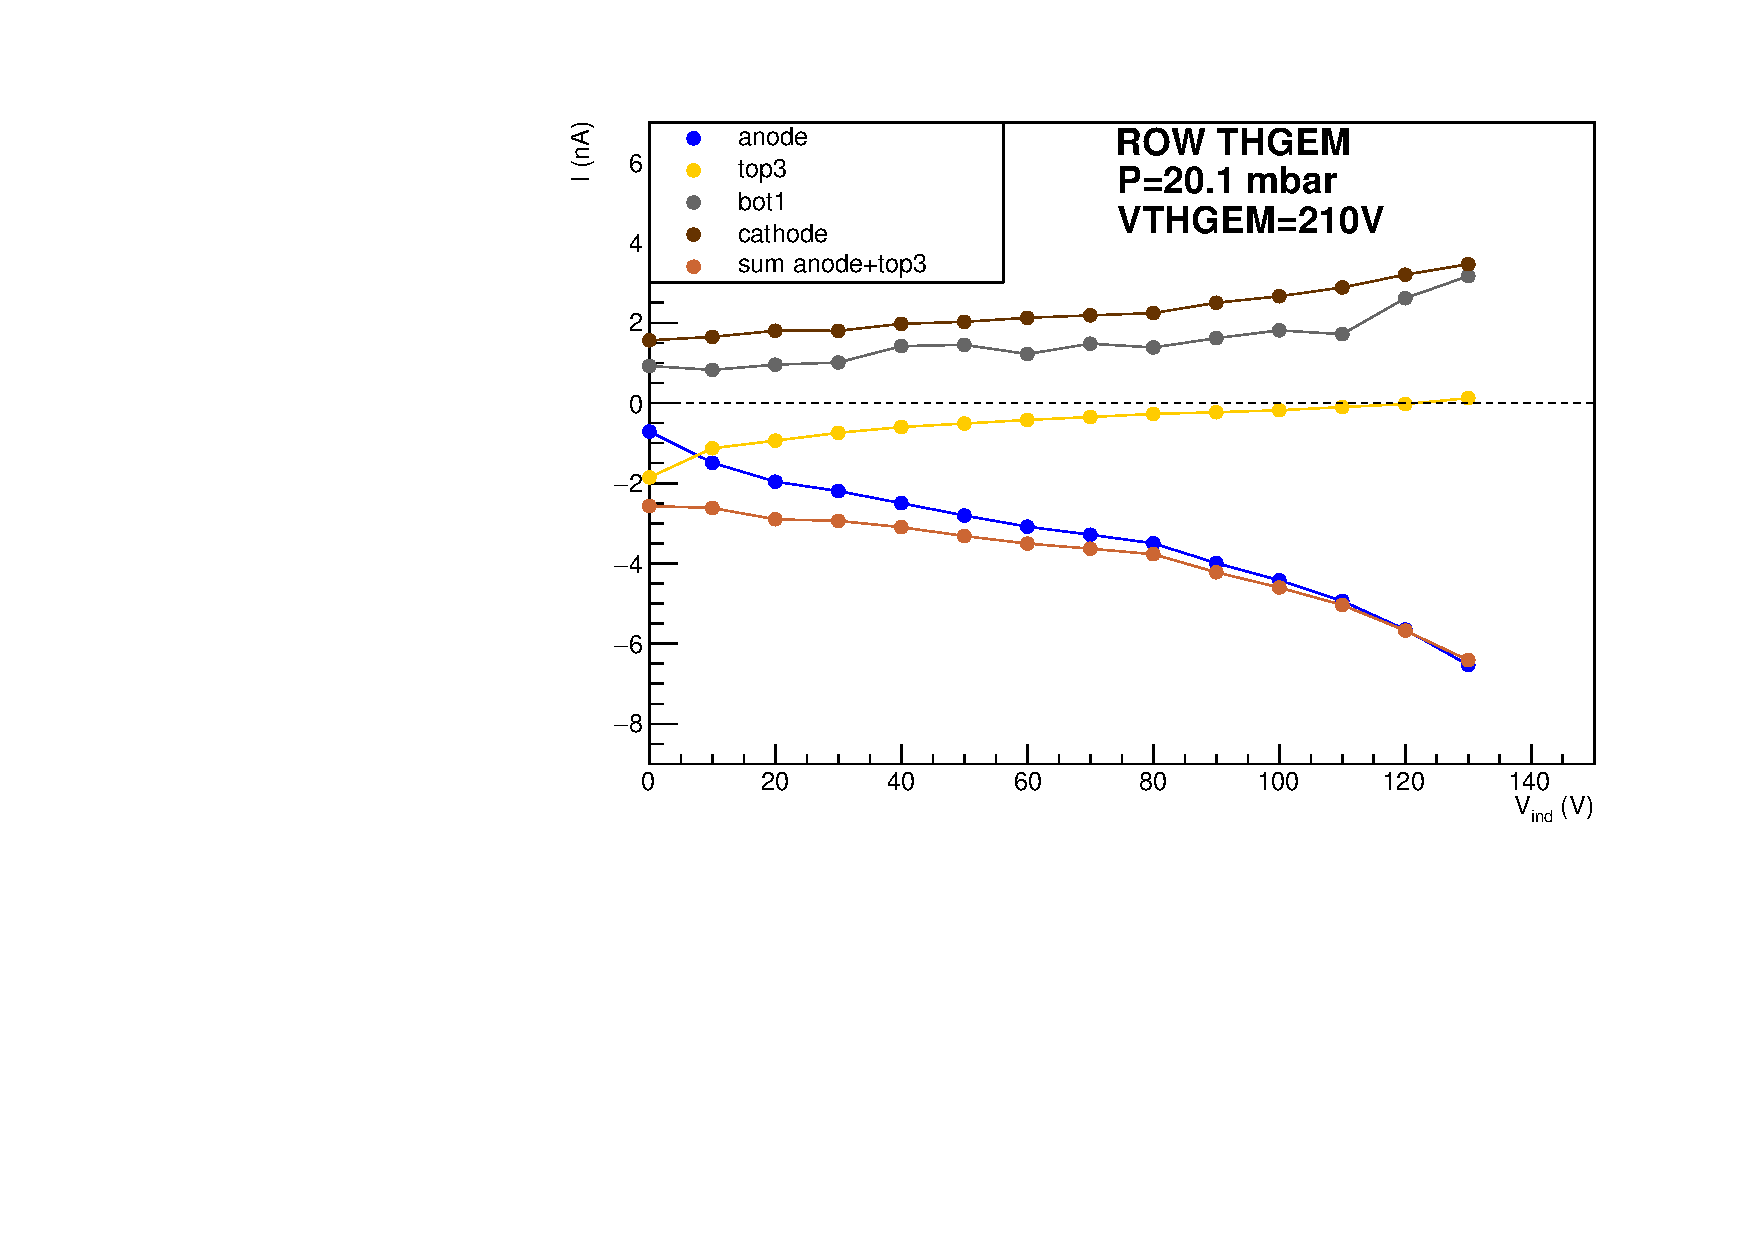
\includegraphics[width=0.96\textwidth]{Immagini/InductionScan_ROW_THGEM_20mbar_bis.pdf}}
	\caption{Currents measured during the scan on the voltage \Vind{} across the induction region at 20~mbar: in (a) \Vthgem{} is at 220~V, in (b) it is at 210~V.}
	\label{fig:induction_ROWTHGEM_20mbar_both}
\end{figure}
Little discharges were observed up to 50~V, while in the range 60$\div$110~V big discharges affected bot1 and top3 currents.
In the case with \Vthgem~=~220~V there is a plateau region from 30 to 70~V, while in that with \Vthgem~=~210~V it is from 30 to 80~V.
\textcolor{red}{giusto?}.
In the former case the optimal value is 50~V, in the latter it is 60~V.



The result of the tests at 30 and 40~mbar are, respectively, shown in Figure~\ref{fig:induction_ROWTHGEM_30mbar} and~\ref{fig:induction_ROWTHGEM_40mbar}.
In the former case the plateau region is clearly visible from 10 to 100~V, so the optimal value is 90~V.
For P~=~40~mbar the plateau region ranges from 20 to 70~V, so the optimal value is 60~V.

%In all the cases the phenomenon of the multiplication 
As for the FULL THGEM, when \Vind{} reaches sufficiently high values, the sum of anode and top3 currents increases, so that the phenomenon of the extension of the multiplication region out of the THGEM holes appears also for the ROW THGEM.

\begin{figure}[!htb]
	\centering
	\subfigure[]{ \label{fig:induction_ROWTHGEM_30mbar} 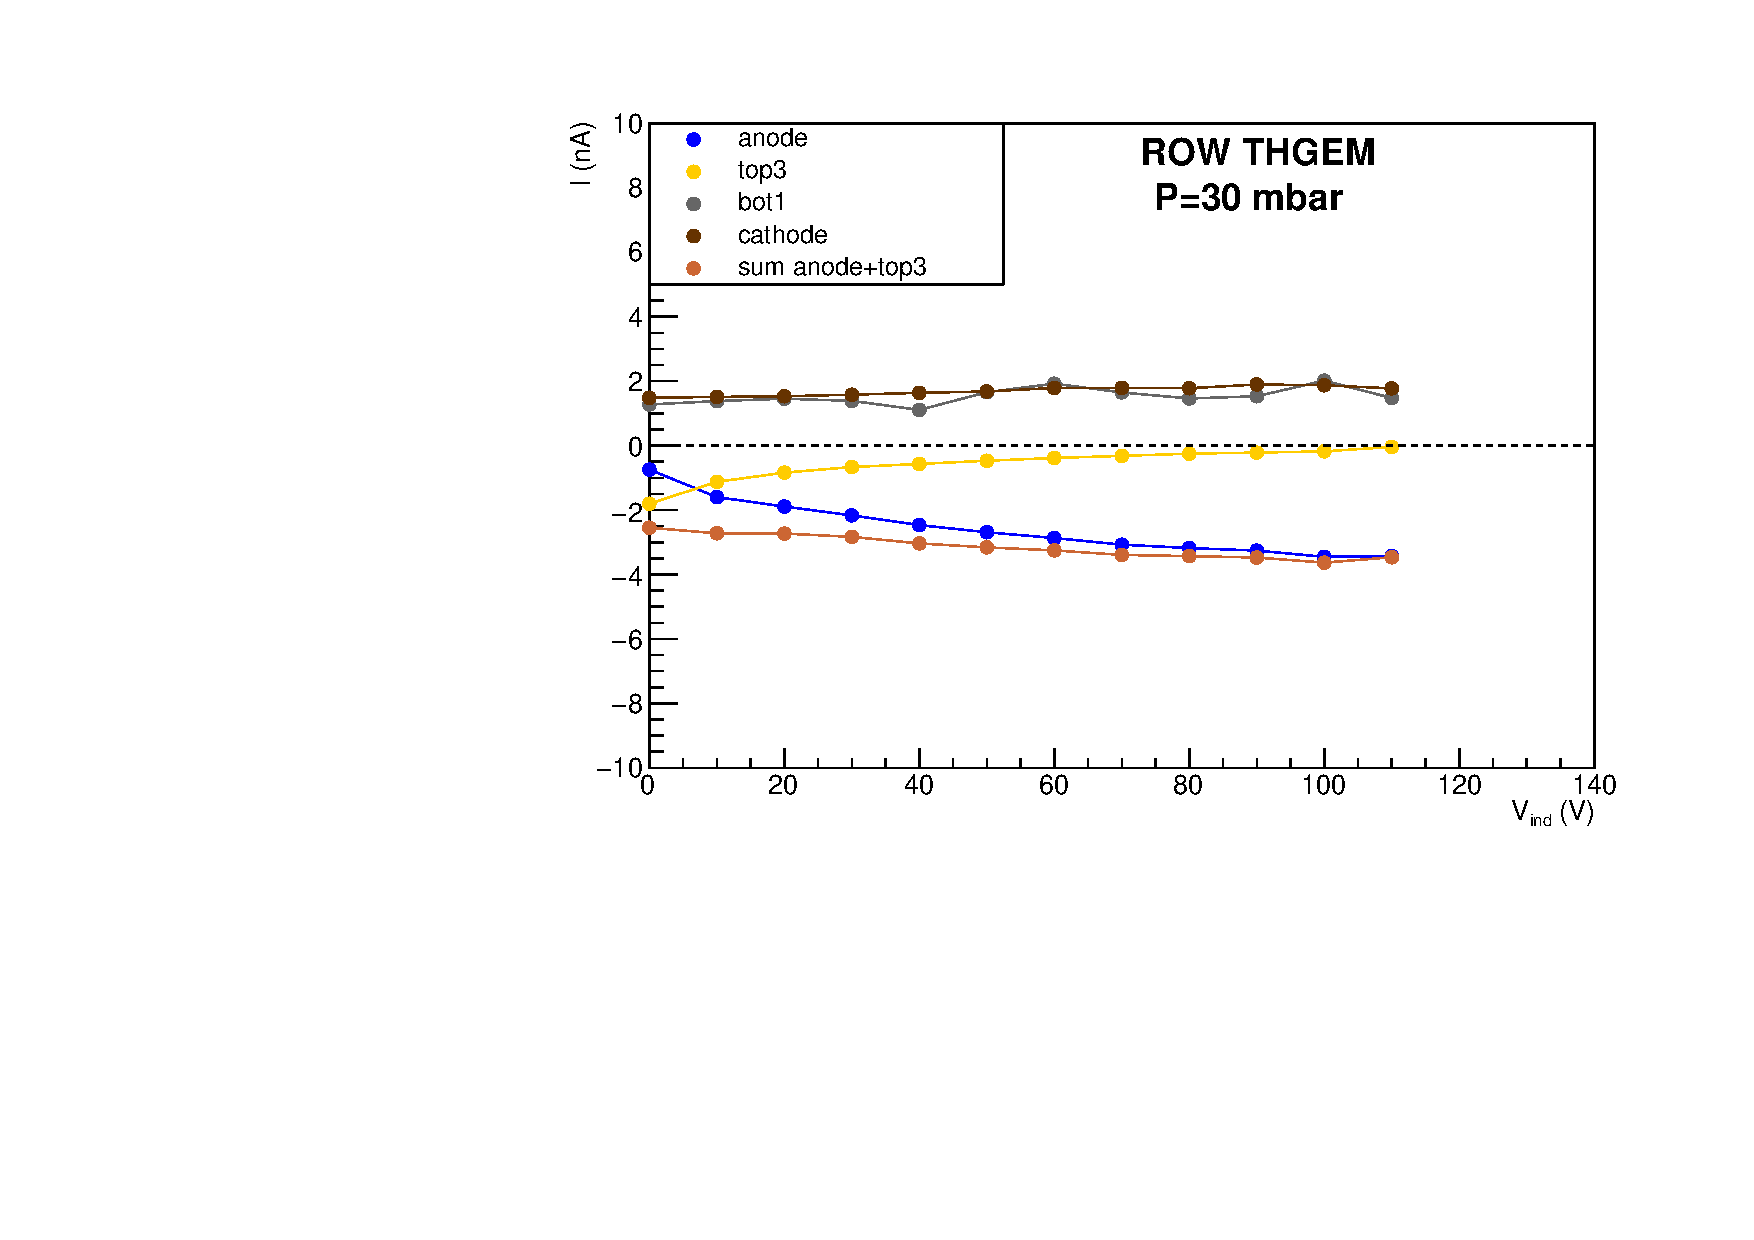
\includegraphics[width=0.96\textwidth]{Immagini/InductionScan_ROW_THGEM_30mbar.pdf}}
	\subfigure[]{ 	\label{fig:induction_ROWTHGEM_40mbar} 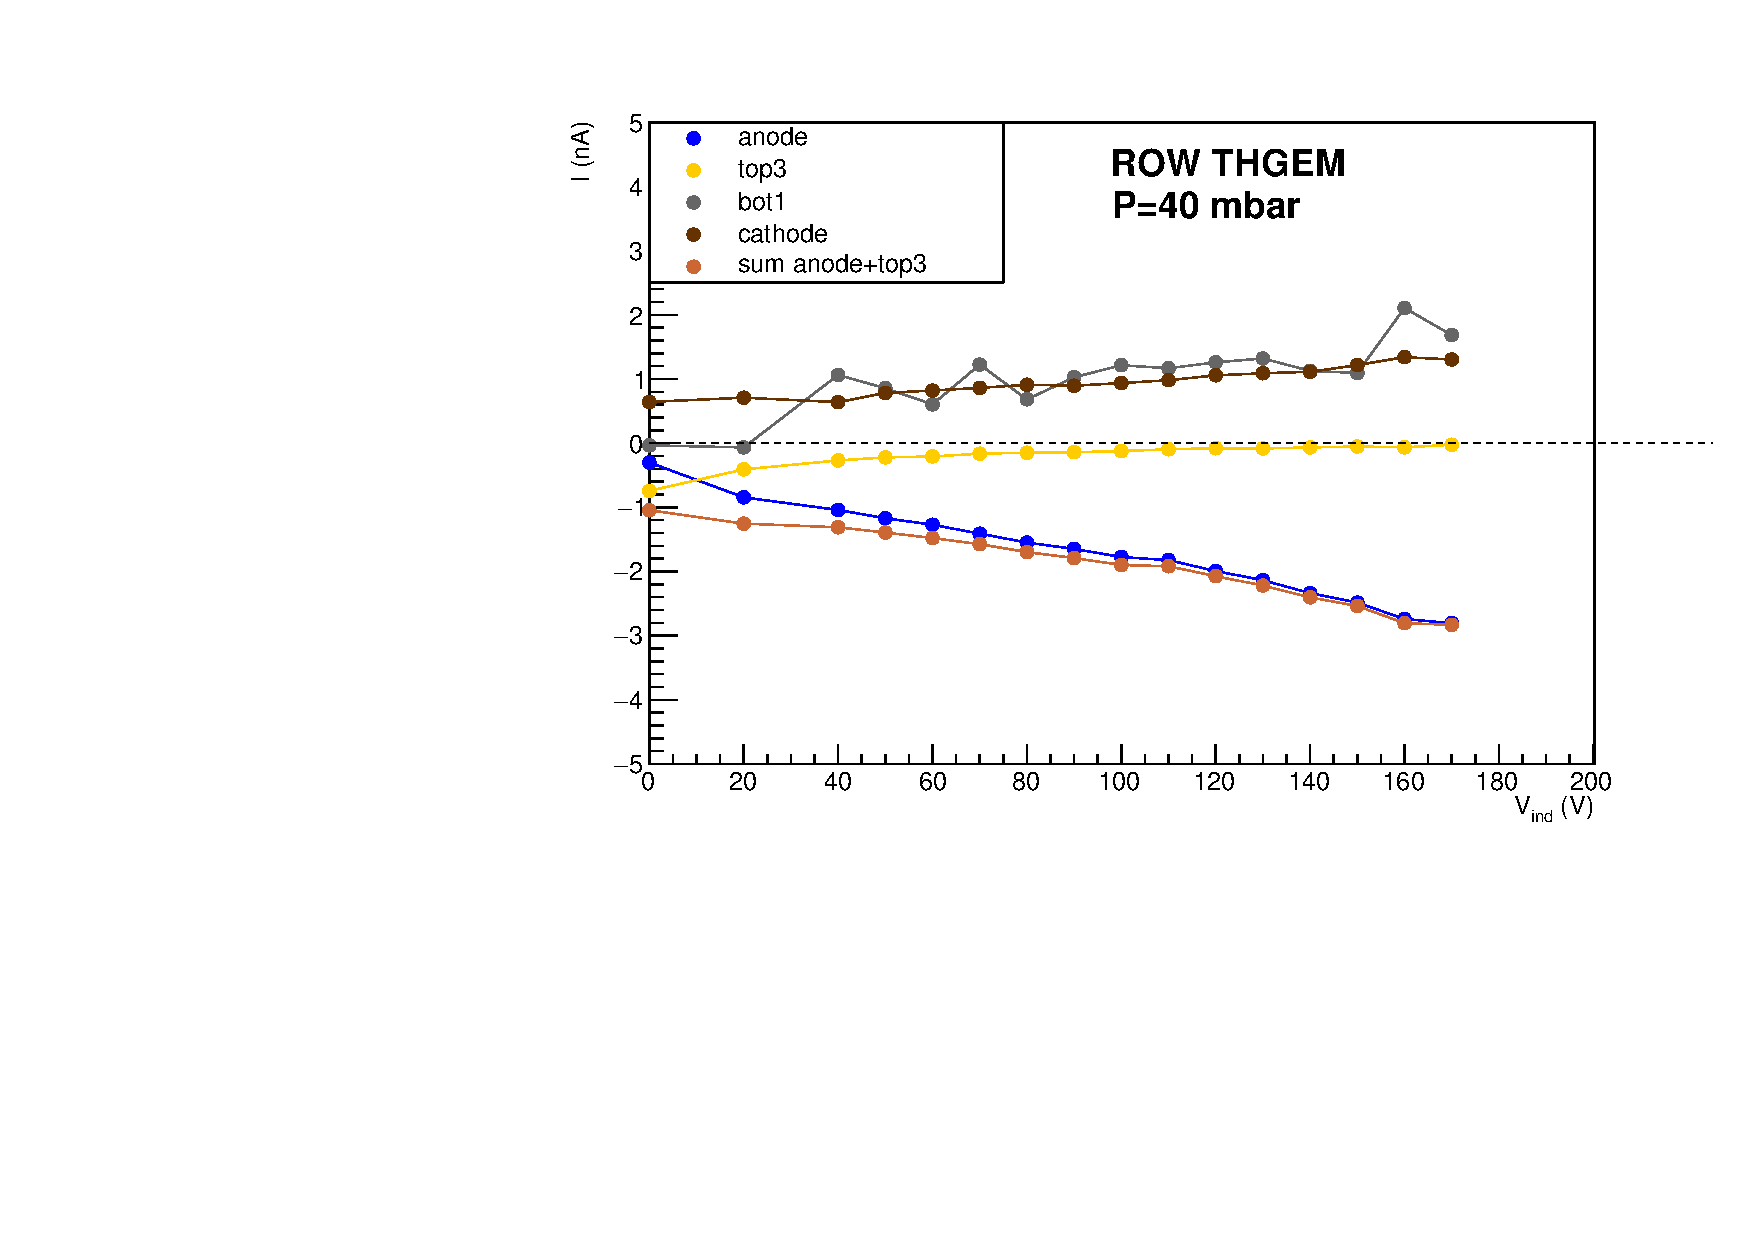
\includegraphics[width=0.96\textwidth]{Immagini/InductionScan_ROW_THGEM_40mbar.pdf}}
	\caption{Currents measured during the scan on the voltage \Vind{} across the induction region: in (a) at 30~mbar, in (b) at 40~mbar.}
	\label{fig:induction_ROWTHGEM_other_pressures}
\end{figure}


%\begin{figure}[htbp]
%	\centering
%	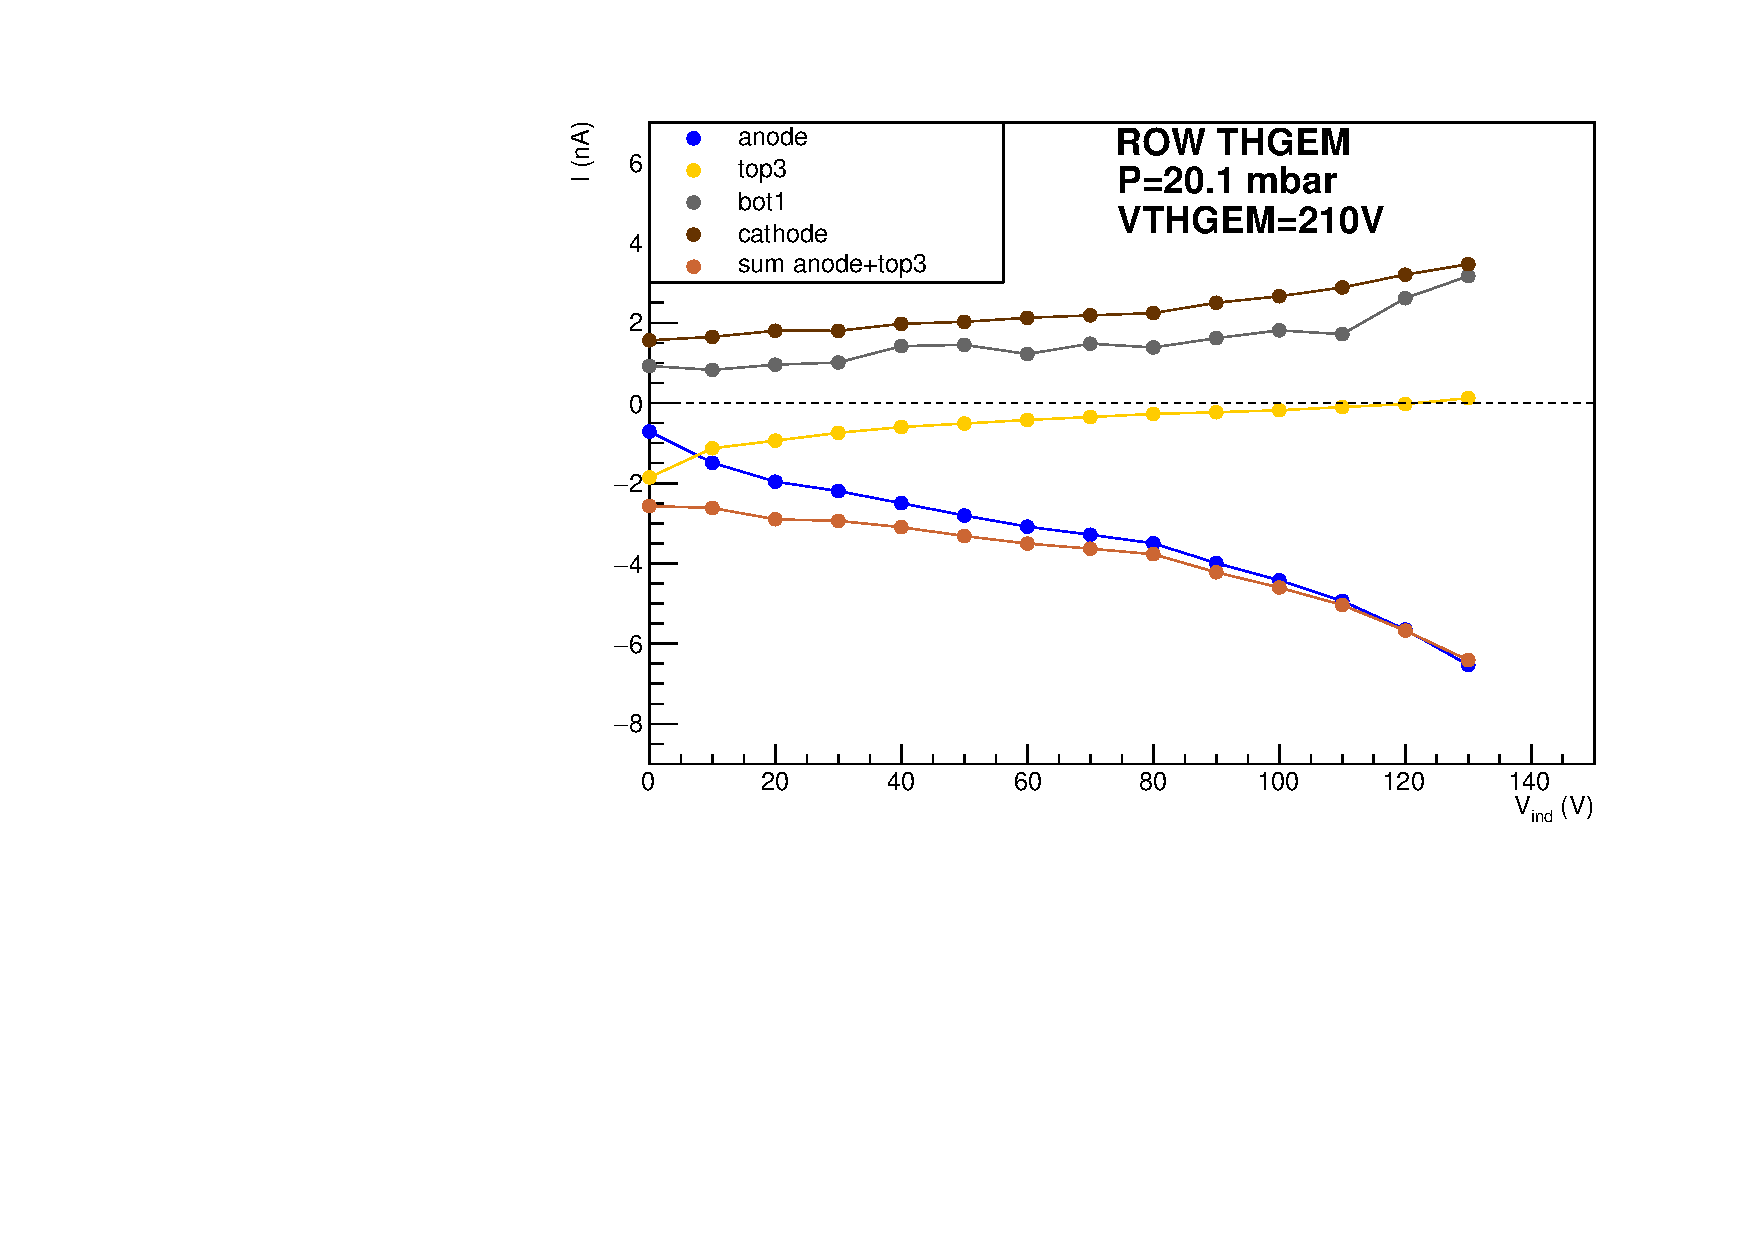
\includegraphics[width=\textwidth]{Immagini/InductionScan_ROW_THGEM_20mbar_bis.pdf}
%	\caption{Currents measured during the scan on the voltage \Vind{} across the induction region at 20~mbar and with \Vthgem{}~=~210~V.}
%	\label{fig:induction_ROWTHGEM_20mbar_bis}
%\end{figure}

%\subsubsection*{Scan at 20 mbar}
%The induction and THGEM scan where repeated at 20~mbar for ROW THGEM and the currents curve show the same behaviour as shown in Figure~\ref{fig:induction_ROWTHGEM_20mbar}. In \Vind~scan, \Vthgem~=~220~V and \Vdrift~=~800~V but plateau is absent. Little discharges were visible up to \Vind~50V while big discharges in the range 60-110V affected bot1 and top3 currents. The optimal value is 50V. In \Vthgem~scan, \Vind~=~50~V and \Vdrift~=~800~V and the last measurable signal was at 180~V. At 225~V there were big discharges, so the optimal \Vthgem~value is 210~V. We do not know if this value is the right one because no drift scan was made. 


\clearpage

\subsubsection{Scan on \Vthgem}

In order to study the multiplication factor of the ROW THGEM in different conditions, a series of measurements was conducted varying the voltage \Vthgem, while pressure, \Vind{} and \Vdrift{} were set to fixed values.
The chosen values of pressure, \Vind{} and \Vdrift{} are shown in Table~\ref{tab:ROWTHGEM_vthgem}.
The \Vthgem{} explored range depends on the selected pressure and on \Vind{} and \Vdrift: for the sake of simplicity these ranges are summarized in Table~\ref{tab:ROWTHGEM_vthgem}.
The increments were ranging from 5 to 10~V.


\begin{table} [htbp]
	\begin{center}
		\renewcommand{\arraystretch}{1.2}
		\begin{tabular} {ccccccc}
			P (mbar) & & \Vind{} (V) & & \Vdrift{} (V) & & \Vthgem{} range (V)\\
			\toprule[0.1em]
			%\hline
			10	& & 50	& & 200	& & 140$\div$205 \\
			20	& &	50	& &	800 & & 180$\div$225 \\
			22	& & 80	& & 300	& & 120$\div$220 \\
			30	& &	70	& & 800 & & 180$\div$240 \\
			32	& & 70	& &	400	& & 170$\div$245 \\
			42	& & 80	& & 700 & & 220$\div$270 \\

			
			\bottomrule[0.1em]
		\end{tabular}
	\end{center}
	\caption{The values of pressure, \Vind{} and \Vdrift{} adopted for the study on \Vthgem{} and the explored \Vthgem{} range.} \label{tab:ROWTHGEM_vthgem}
\end{table}

%\textcolor{red}{Visto che i grafici sarebbero tanti, sarebbe meglio metterne soltanto due o tre pi\F9 esemplificativi?}

The results of the scans at 10 and 32~mbar are shown, respectively, in Figure~\ref{fig:thgem_ROWTHGEM_10mbar} and~\ref{fig:thgem_ROWTHGEM_30mbar_bis}: the typical exponential growth of the currents is verified also for the ROW THGEM.
 

\begin{figure}[!htb]
	\centering
	\subfigure[]{ \label{fig:thgem_ROWTHGEM_10mbar} 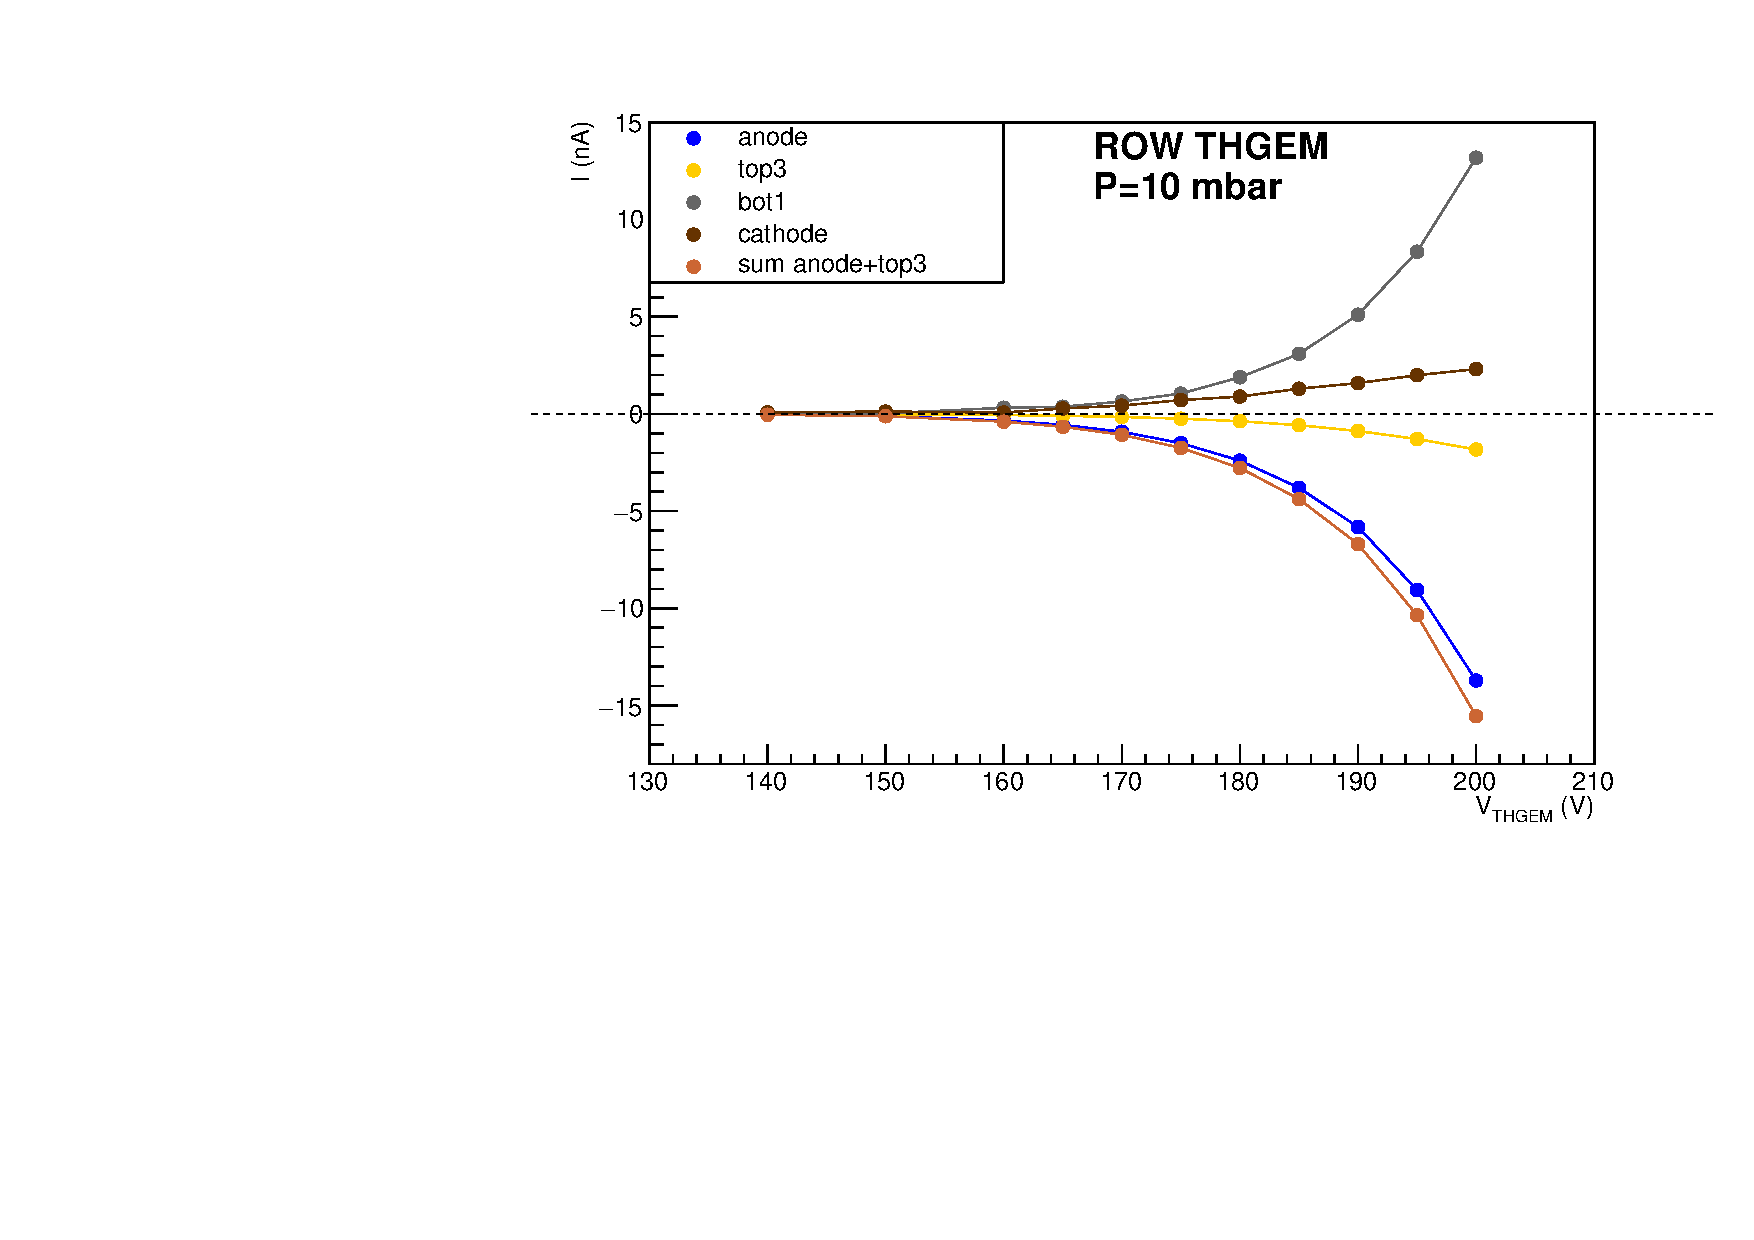
\includegraphics[width=0.96\textwidth]{Immagini/thgemScan_ROW_THGEM_10mbar.pdf}}
	\subfigure[]{ 	\label{fig:thgem_ROWTHGEM_30mbar_bis} 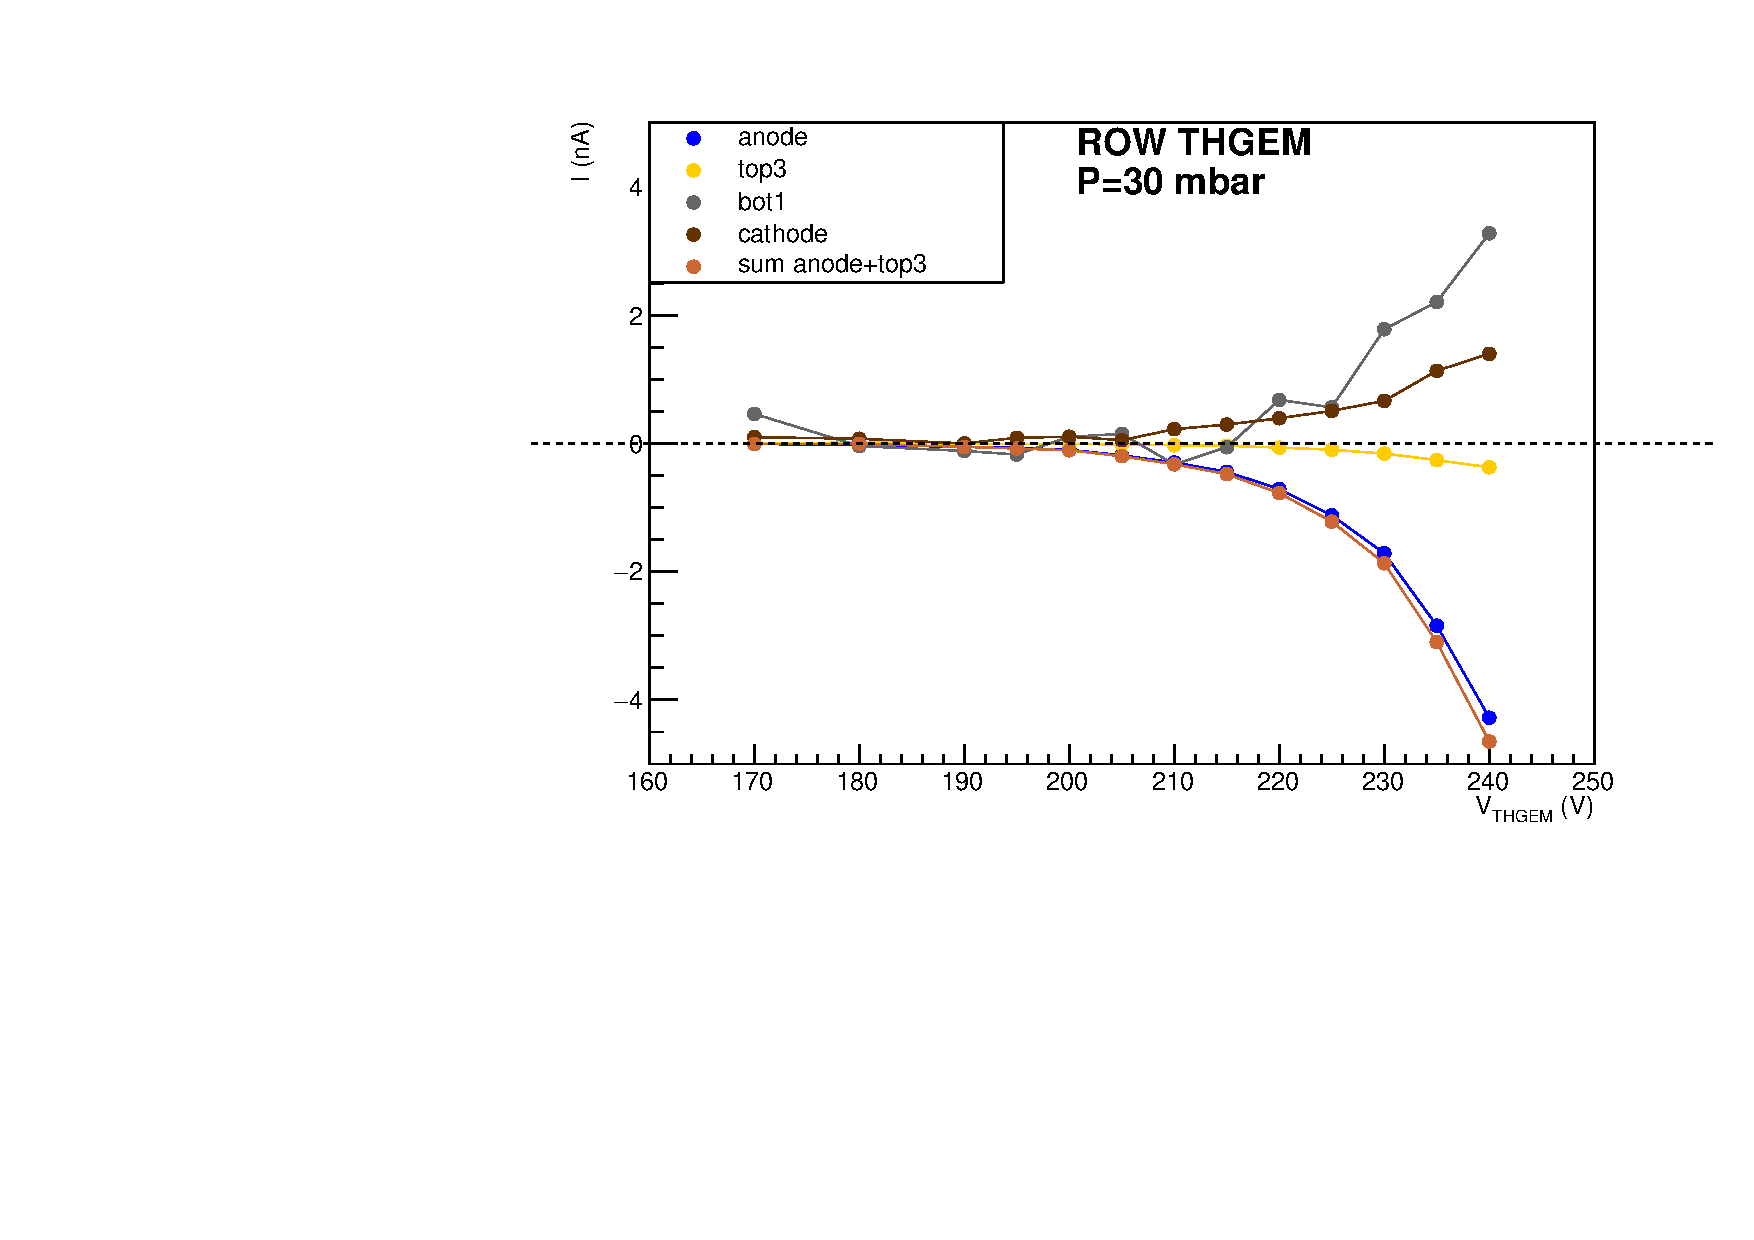
\includegraphics[width=0.96\textwidth]{Immagini/thgemScan_ROW_THGEM_30mbar_bis.pdf}}
	\caption{Currents measured during the scan on the voltage \Vthgem{} across each ROW THGEM: in (a) at 10~mbar, in (b) at 32~mbar.}
	\label{fig:thgem_ROWTHGEM}
\end{figure}


From these measurements, the multiplication factors of the ROW THGEM were evaluated as a function of \Vthgem{} and pressure. 




\begin{figure}[!t]
	\centering
	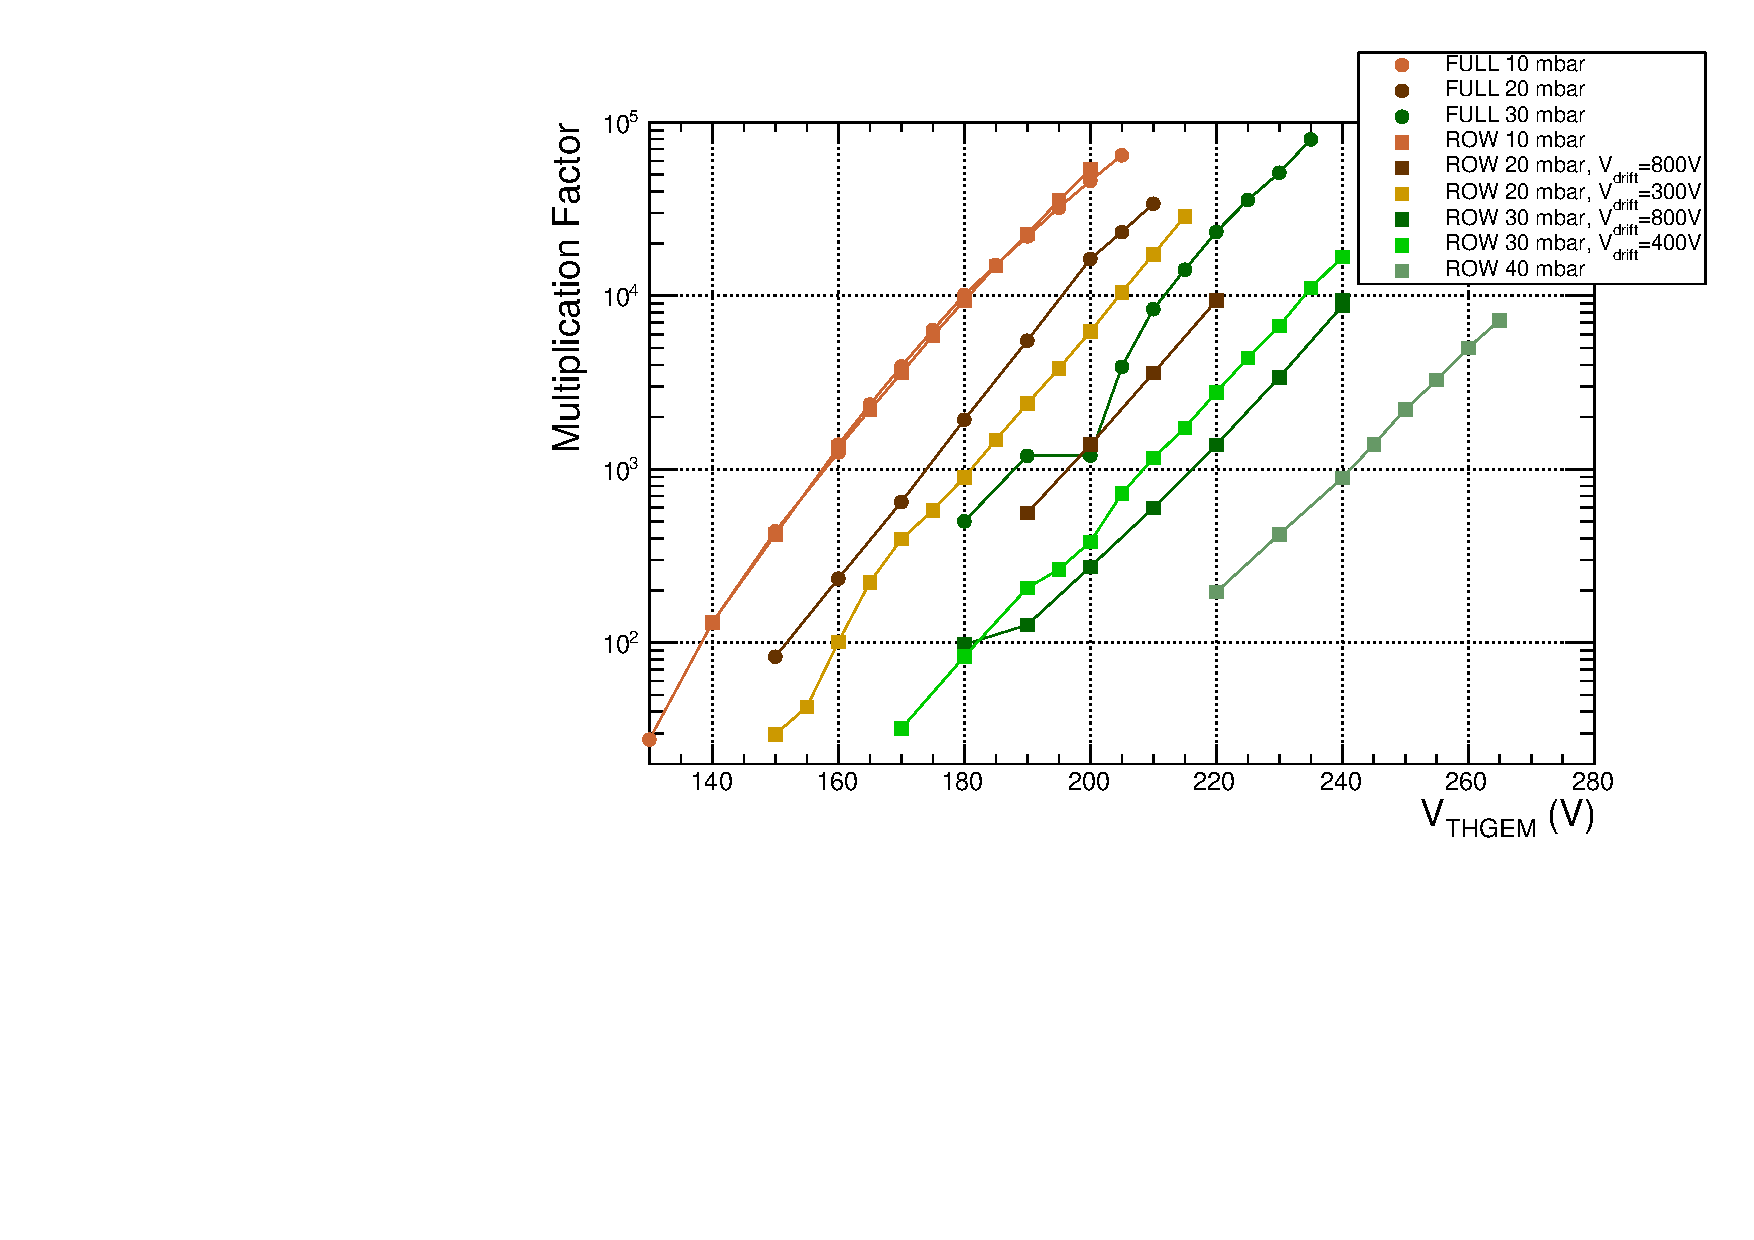
\includegraphics[width=\textwidth]{Immagini/MFvsTHGEM_FULLandROW_bis.pdf}
	\caption{Comparison between the multiplication factors evaluated for the ROW THGEM (square) and those for the FULL THGEM (circle) as a function of \Vthgem{} and pressure.}
	\label{fig:multiplication_factor_FULLandROW}
\end{figure}










\clearpage

\subsubsection{Scan on \Vdrift}

To fully characterize the tracker response, a study was conducted varying the potential difference \Vdrift{} across the drift region, while pressure, \Vind{} and \Vthgem{} were kept fixed.
The explored range goes from 0~V (or 100~V in the case with P~=~20~mbar) to the discharge voltage, which depends on the gas pressure: for P~=~30~mbar it was 1400~V, for P~=~20~mbar it was 1000~V, and for P~=~11~mbar it was 800~V.
The increments were of 100~V for all the cases, but for P~=~11~mbar the first 400~V were scanned in step of 30~V.
In Table~\ref{tab:ROWTHGEM_vdrift} the adopted value of pressure, \Vind{} and \Vthgem{} are shown.


\begin{table} [!h]
	\begin{center}
		\renewcommand{\arraystretch}{1.2}
		\begin{tabular} {ccccc}
			P (mbar) & & \Vind{} (V) & & \Vthgem{} (V)\\
			\toprule[0.1em]
			%\hline
			30	& &	70	& &	240 \\
			30	& &	70	& & 230 \\
			20	& & 80	& & 210 \\
			10	& & 50	& & 180 \\
			
			\bottomrule[0.1em]
		\end{tabular}
	\end{center}
	\caption{The values of pressure (P), \Vind{} and \Vthgem{} adopted for the study on \Vdrift.} \label{tab:ROWTHGEM_vdrift}
\end{table}


The result of the two scans at 30~mbar are shown in Figure~\ref{fig:drift_ROWTHGEM_30mbar_both}: in both cases the measured currents increase rapidly up to 200~V, then they decrease and reach a saturation value. 
\textcolor{red}{Perch�?}


\begin{figure}[!htb]
	\centering
	\subfigure[]{ \label{fig:drift_ROWTHGEM_30mbar} 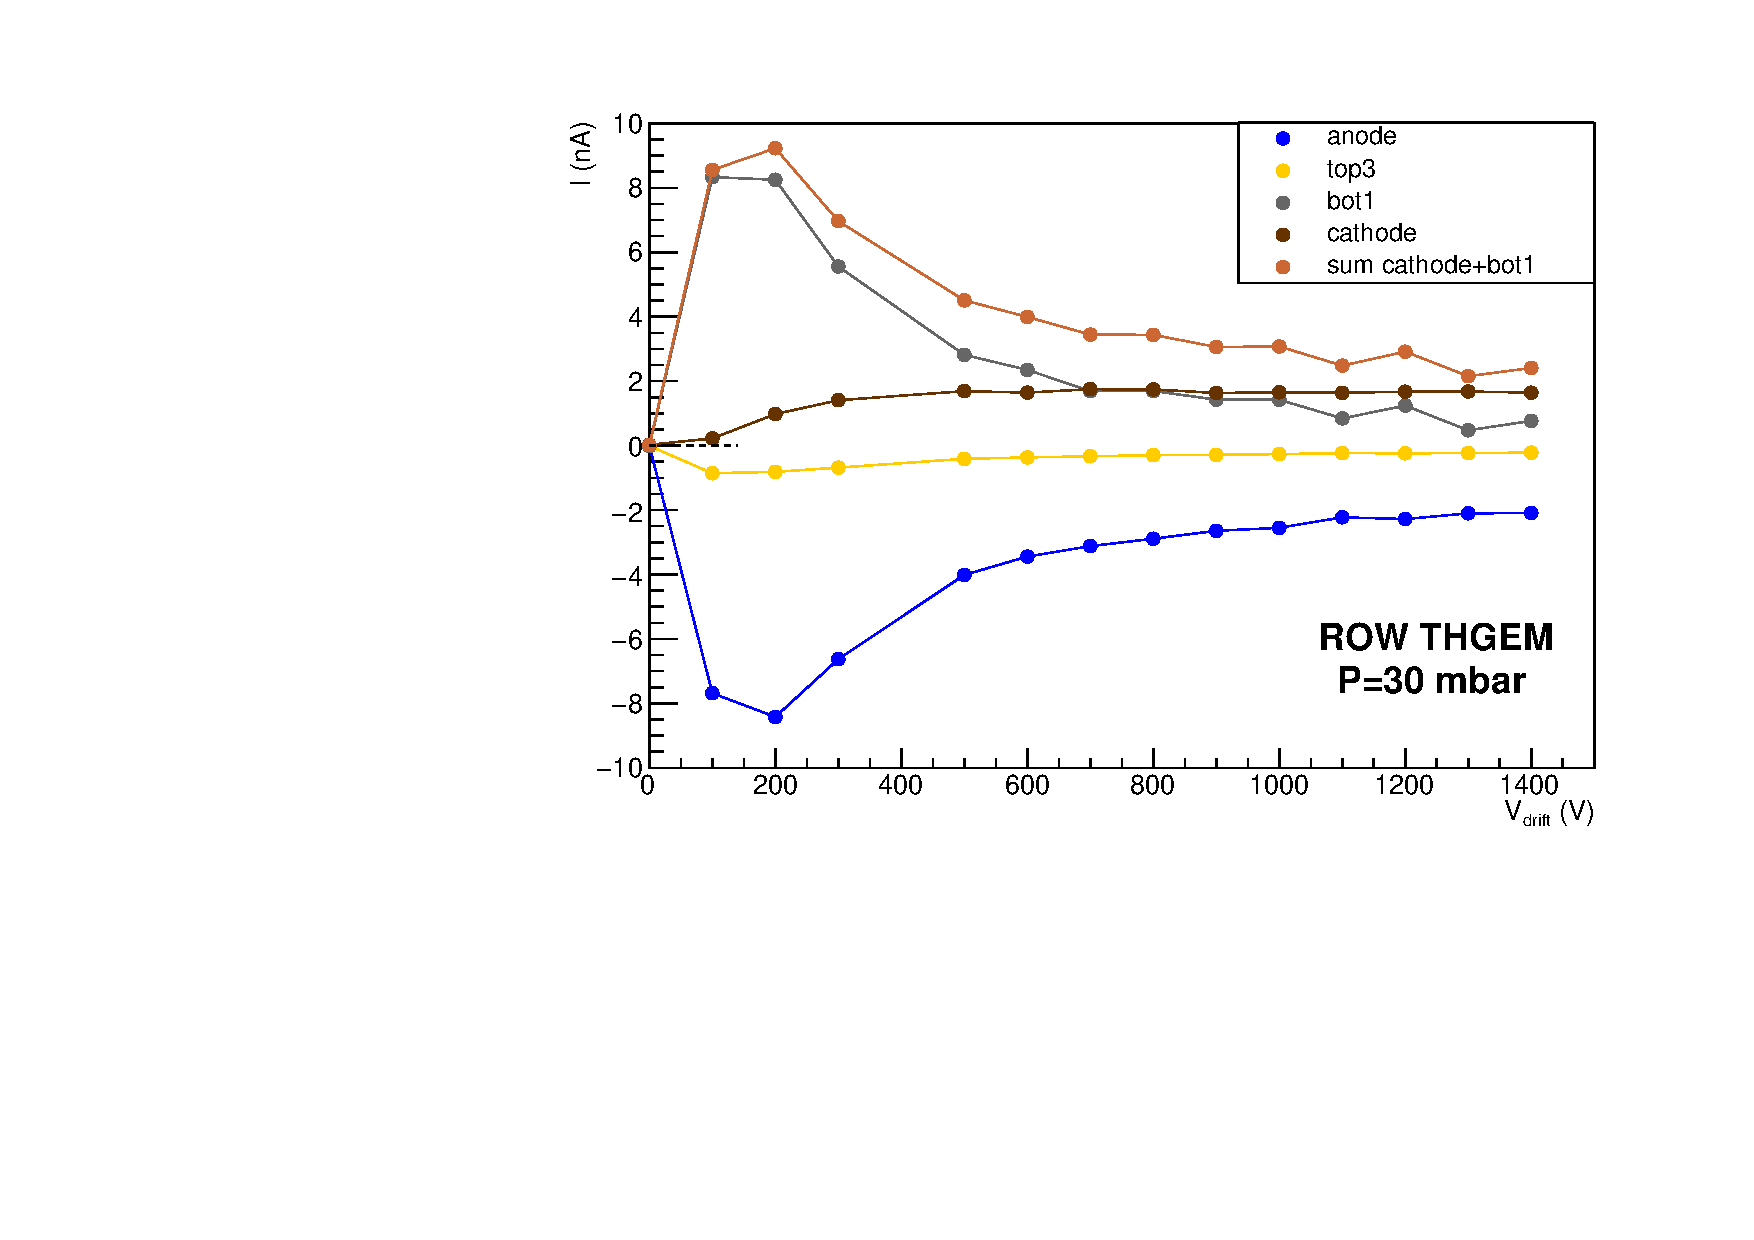
\includegraphics[width=0.96\textwidth]{Immagini/DriftScan_ROW_THGEM_30mbar.pdf}}
	\subfigure[]{ 	\label{fig:drift_ROWTHGEM_30mbar_bis} 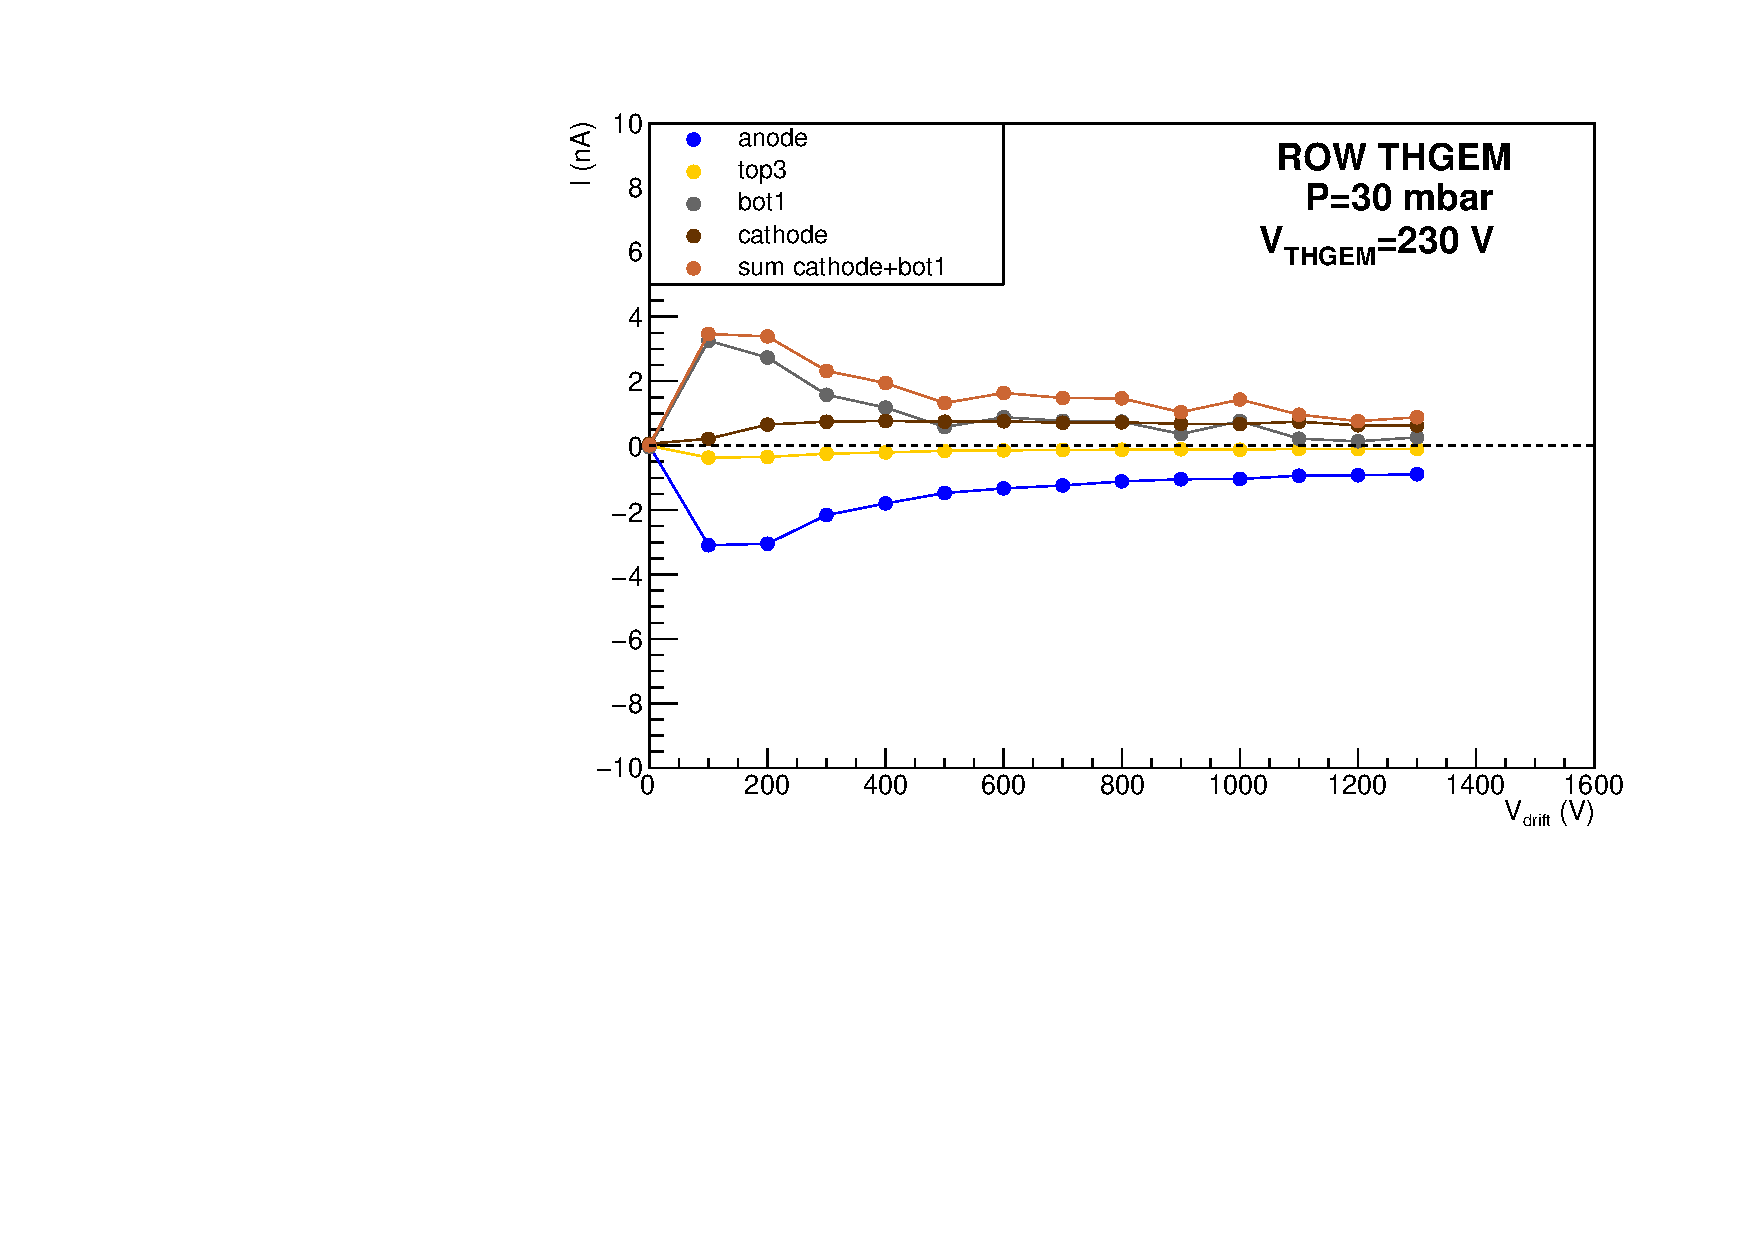
\includegraphics[width=0.96\textwidth]{Immagini/DriftScan_ROW_THGEM_30mbar_bis.pdf}}
	\caption{Currents measured during the scan on the voltage \Vdrift{} across the drift region at 20~mbar: in (a) \Vthgem{} is at 240~V, in (b) it is at 230~V.}
	\label{fig:drift_ROWTHGEM_30mbar_both}
\end{figure}

The same phenomenon appears also in the scans at 20 and 10~mbar, respectively shown in Figure~\ref{fig:drift_ROWTHGEM_20mbar} and~\ref{fig:drift_ROWTHGEM_10mbar}.

\begin{figure}[!htb]
	\centering
	\subfigure[]{ \label{fig:drift_ROWTHGEM_20mbar} 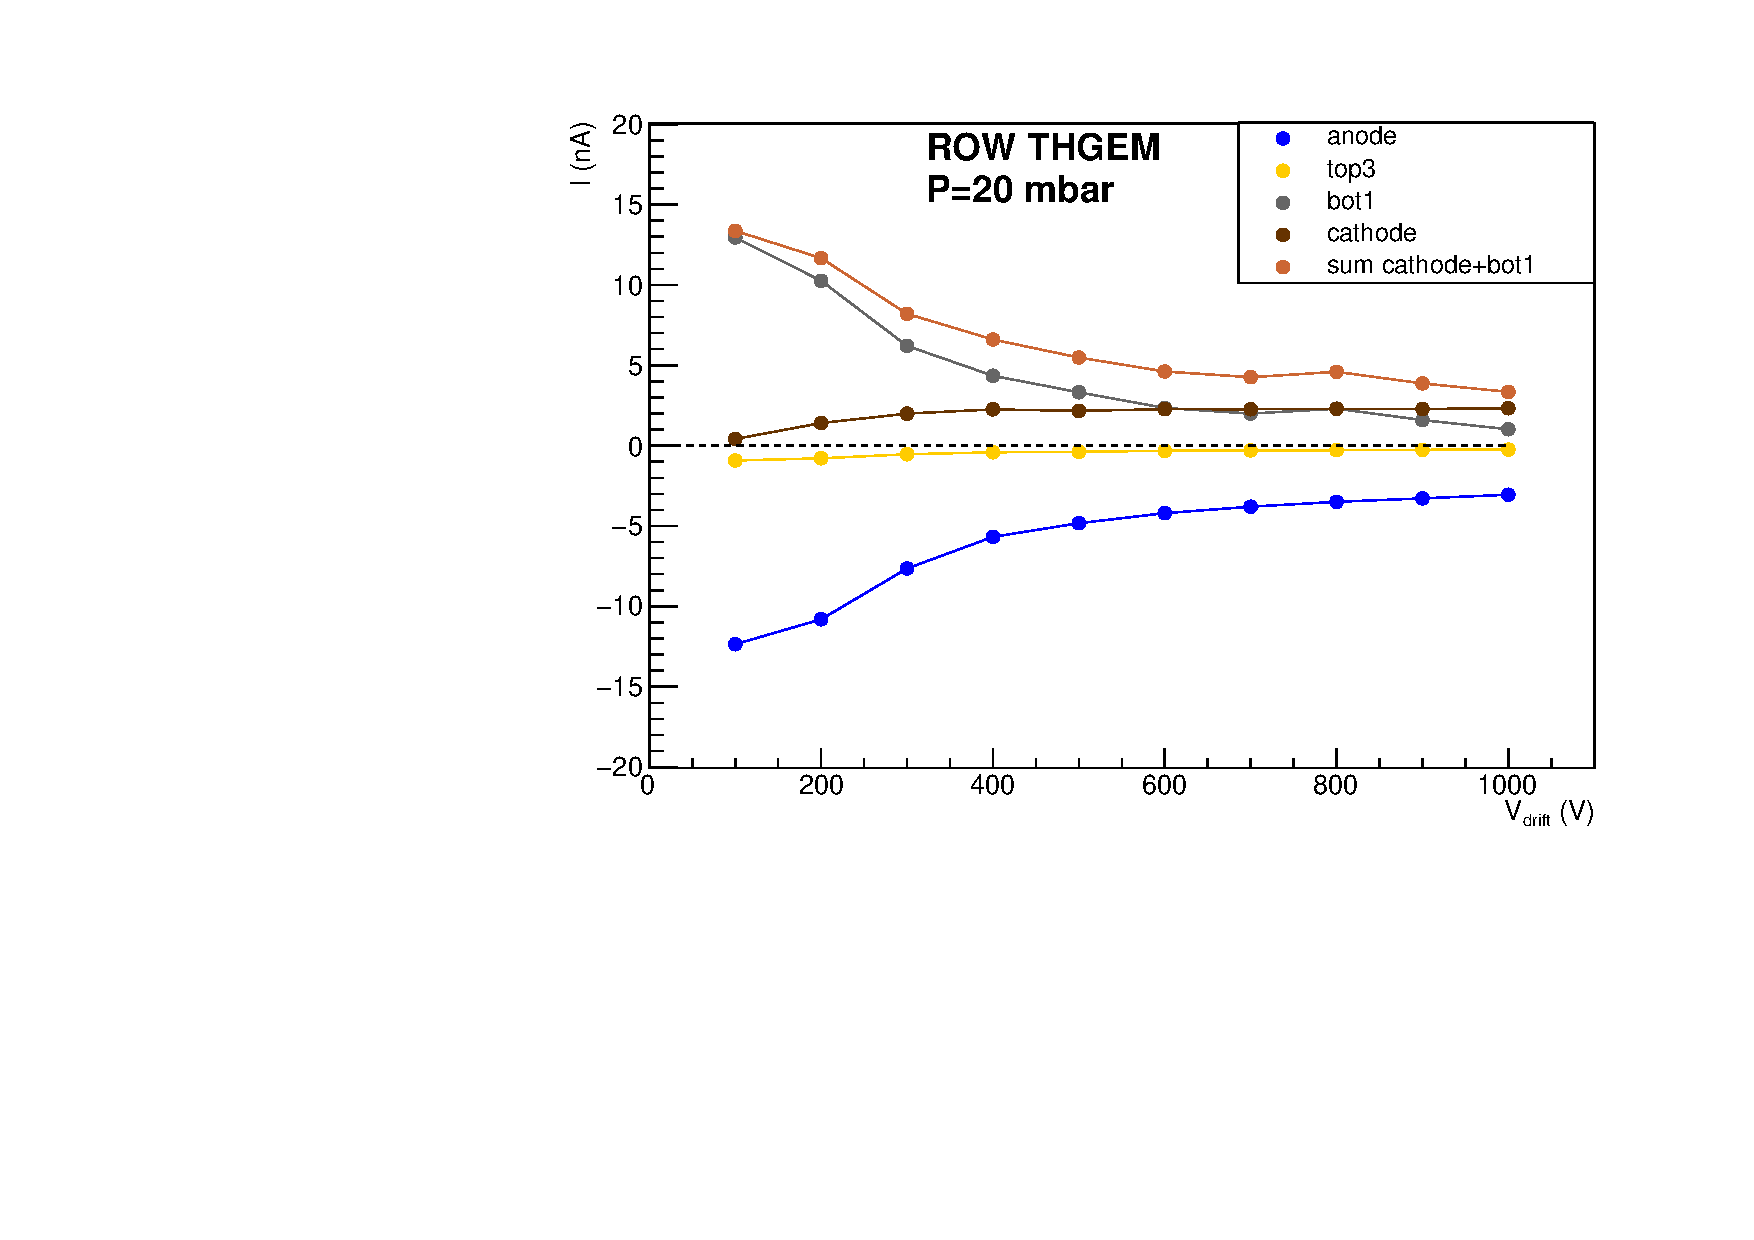
\includegraphics[width=0.96\textwidth]{Immagini/DriftScan_ROW_THGEM_20mbar.pdf}}
	\subfigure[]{ 	\label{fig:drift_ROWTHGEM_10mbar} 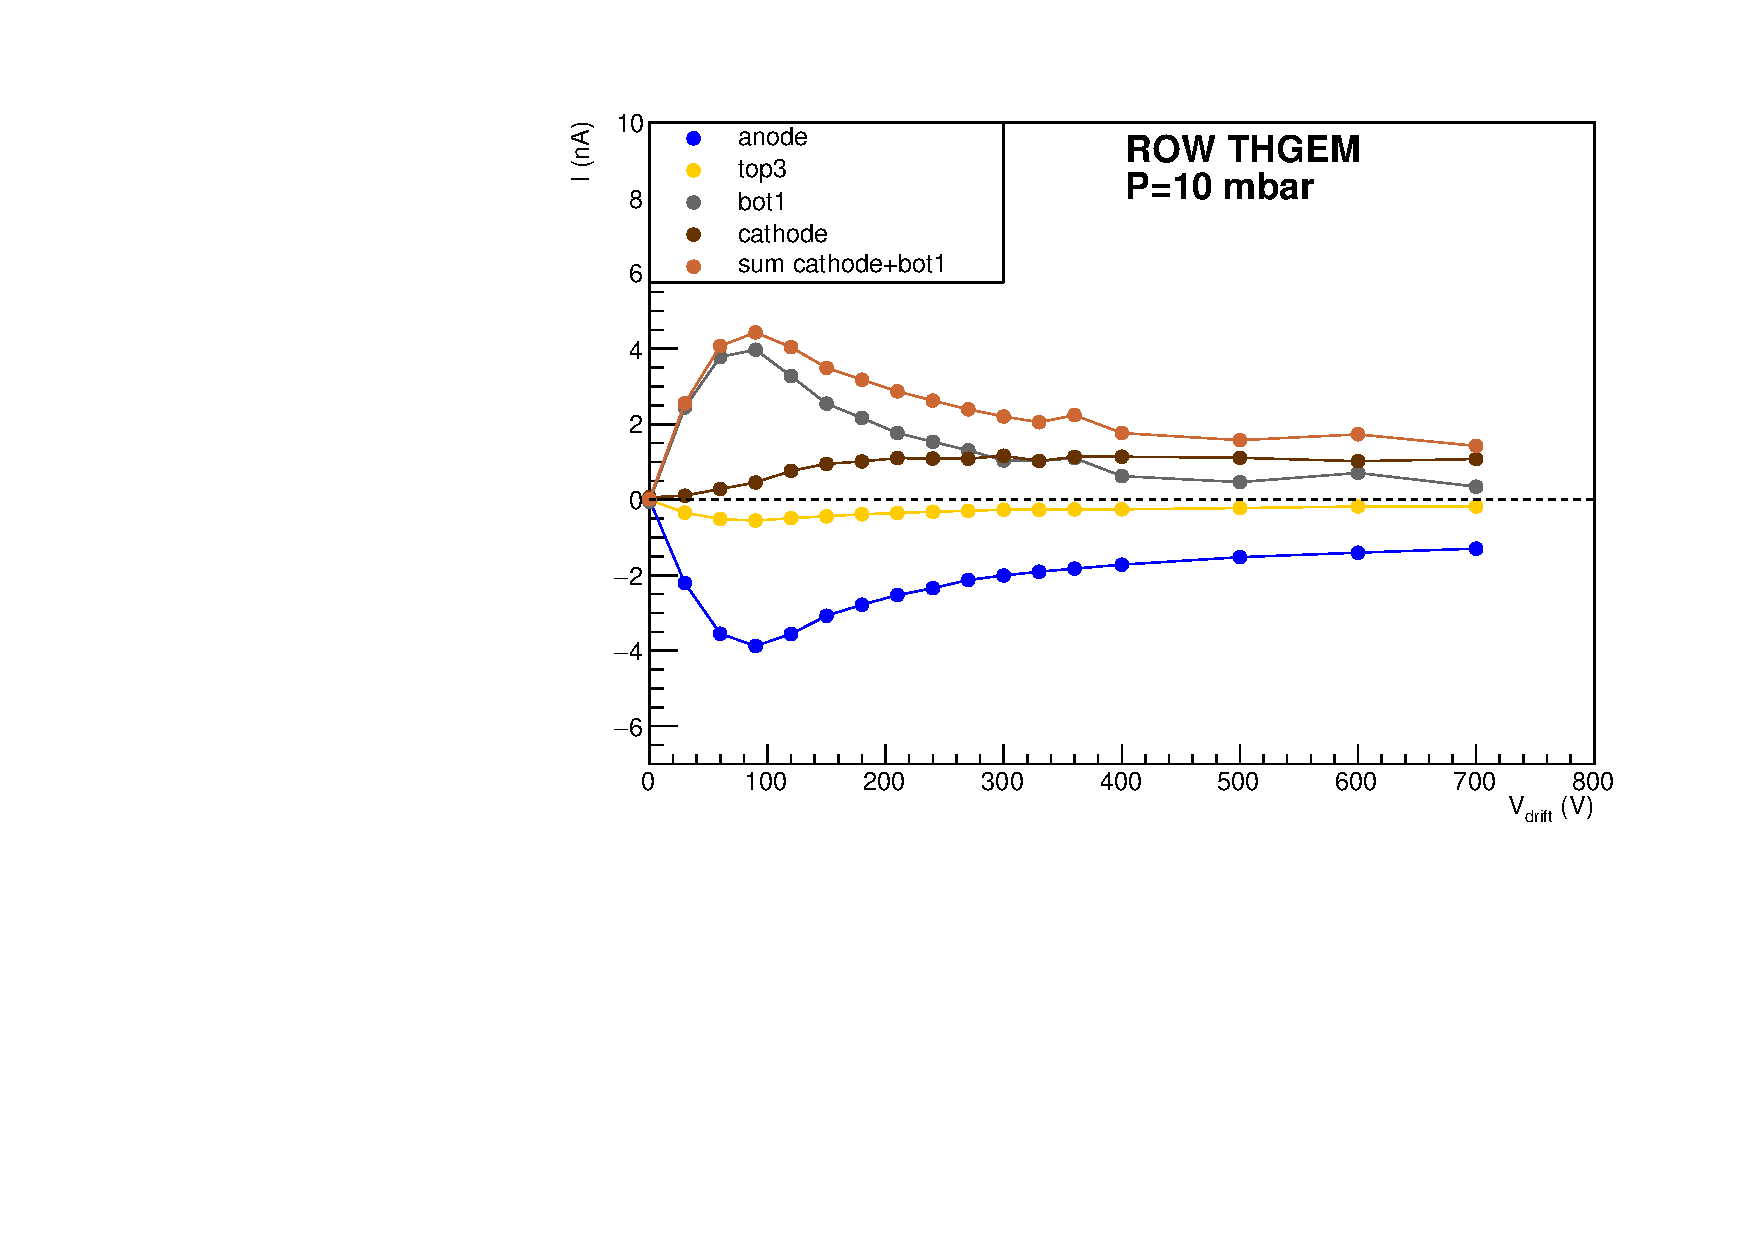
\includegraphics[width=0.96\textwidth]{Immagini/DriftScan_ROW_THGEM_10mbar.pdf}}
	\caption{Currents measured during the scan on the voltage \Vdrift{} across the drift region: in (a) at 20~mbar, in (b) at 10~mbar.}
	\label{fig:drift_ROWTHGEM_20and10_mbar}
\end{figure}



From these measurements, the ion backflow of the ROW THGEM was evaluated as a function of \Vdrift{} and pressure.
The results of the calculation are shown in Figure~\ref{fig:ion_backflow_FULLandROW}: the ion backflow rapidly increases at increasing \Vdrift{} and is much bigger than that of the FULL THGEM.





\begin{figure}[htbp]
	\centering
	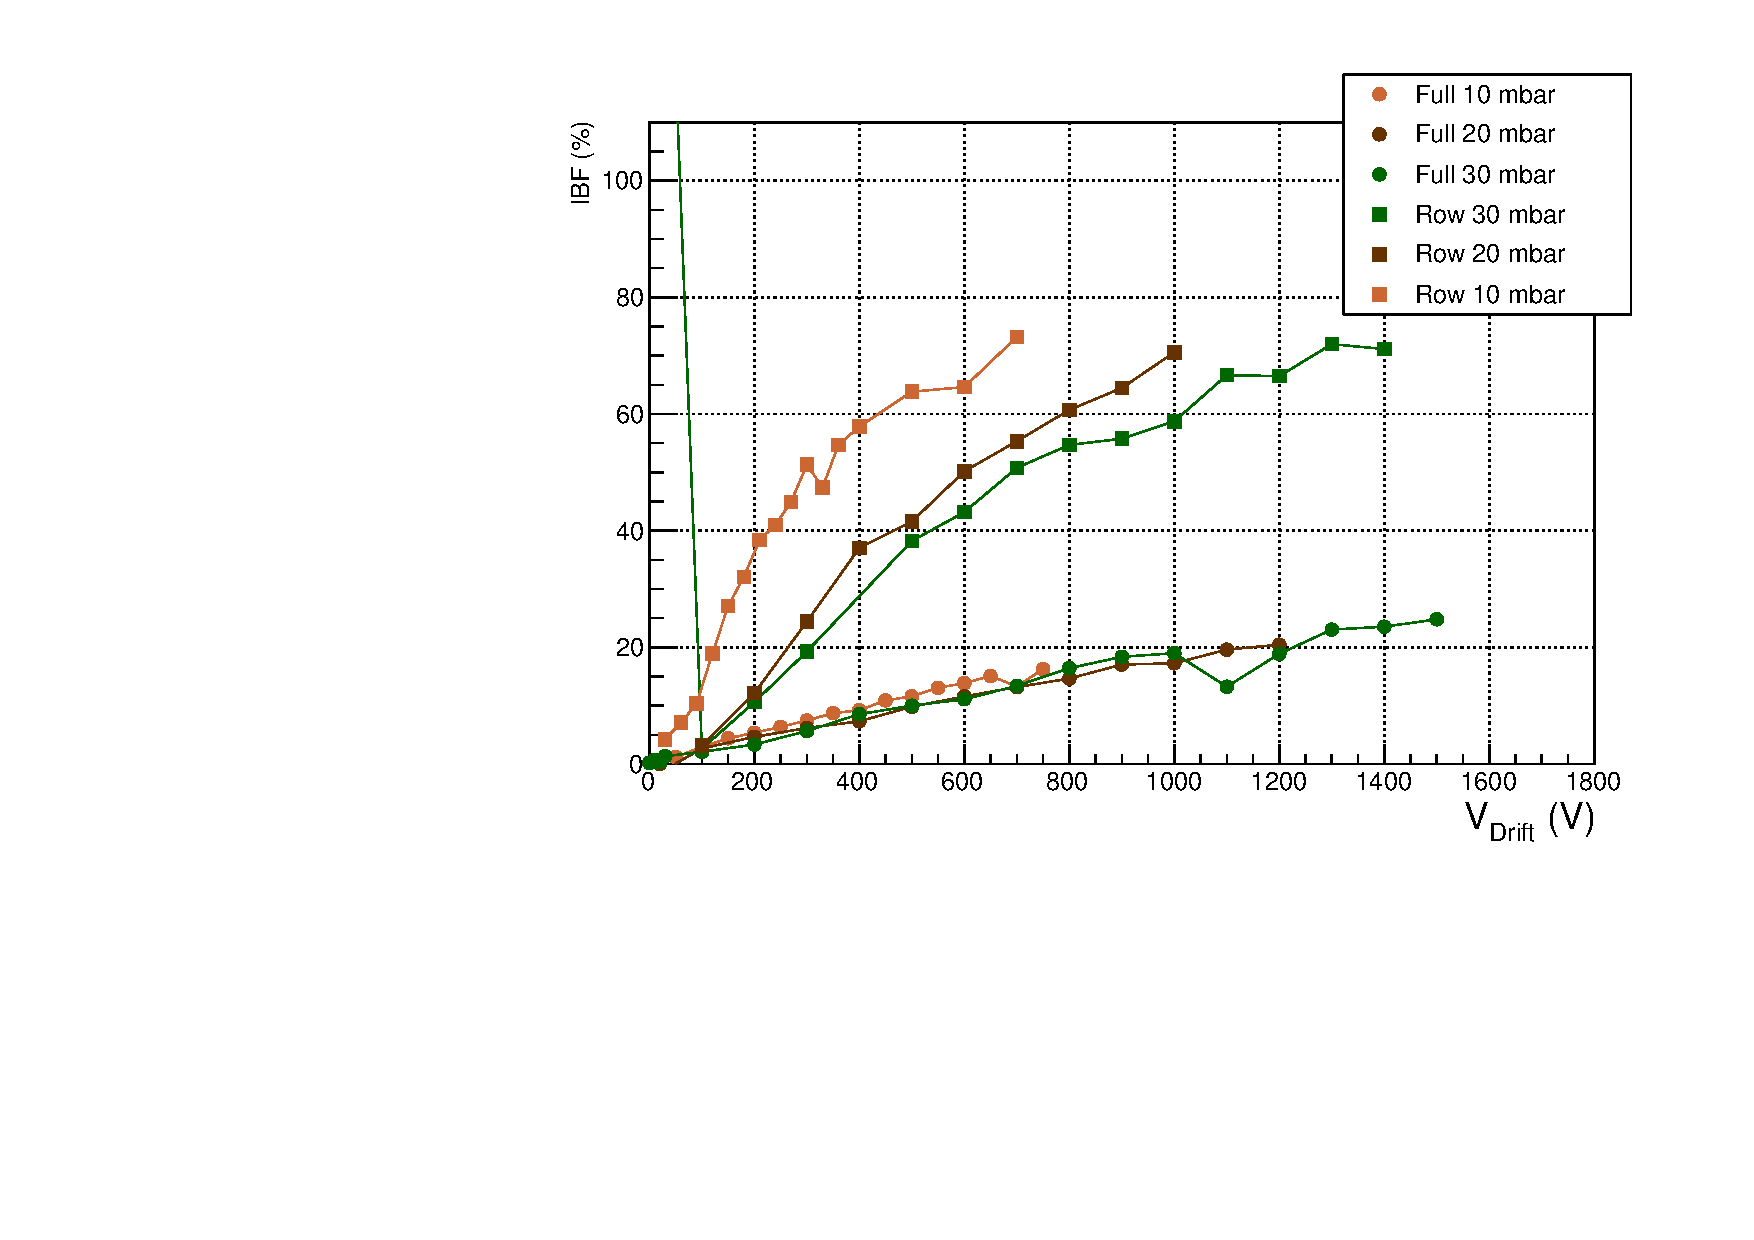
\includegraphics[width=\textwidth]{Immagini/IBFvsDrift_FULLandROW.pdf}
	\caption{Comparison between the ion backflows evaluated for the ROW THGEM (square) and those for the FULL THGEM (circle) as a function of \Vdrift{} and pressure.}
	\label{fig:ion_backflow_FULLandROW}
\end{figure}







\clearpage

\subsection{New test with $\alpha$ source} \label{sec:new_test_alpha}

%%% PARTE AGGIUNTA DA IRENE 27/02/2020
On February 20 2020 another test with $\alpha$ source was done in the same condition of test with beam (see Section~\ref{sec:test_beam}). 

\subsubsection{Scan on \Vthgem}

The new scan on \Vthgem{} was conducted fixing P~=~9.3~mbar, \Vind{} = 50 V and \Vdrift{} = 400 V.
The measured currents have the same behaviour of the previous tests. 
%The difference is that the maximum anodic achievable current: ~20 nA fixing \Vind{} = 50 V and \Vdrift{} = 400 V and ~40 nA fixing \Vind{} = 70 V and \Vdrift{} = 600 V.
%Comparing these results with Figure~\ref{fig:thgem_FULLTHGEM_10mbar}, 
Comparing this scan with a previous one done in similar conditions (P~=~11~mbar, \Vind{} = 70 V, \Vdrift{} = 600 V), which is shown in Figure~\ref{fig:thgem_FULLTHGEM_10mbar}, the relative distance between the anodic and the top3 current is smaller.
This is due to the different values of \Vind{}, that change the fraction of electrons that can reach the anode respect to the number of electrons produced in total.
\begin{figure}[p]
	\centering
	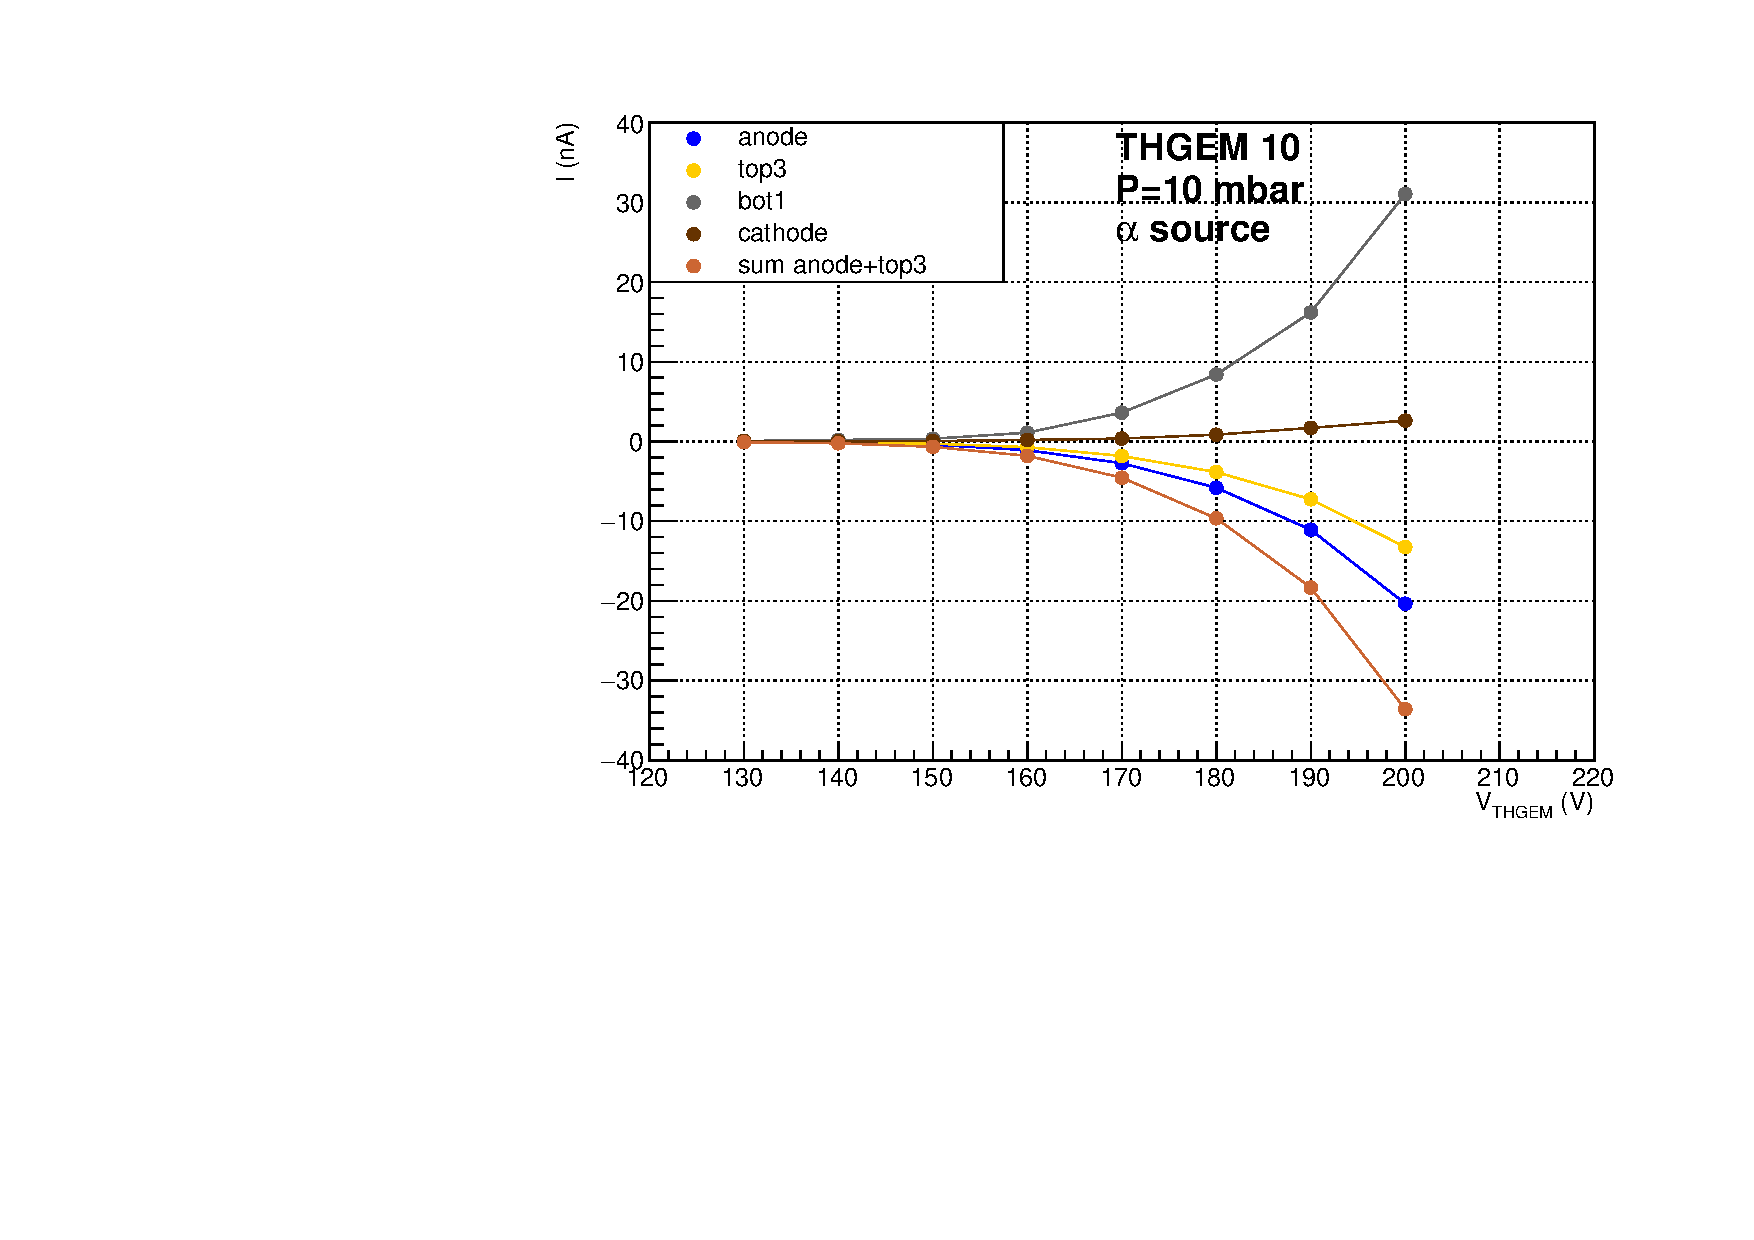
\includegraphics[width=\textwidth]{Immagini/thgemScan_THGEM10_10mbar_bis.pdf}
	\caption{Currents measured during the scan on the voltage \Vthgem{} across each FULL THGEM at 9.3~mbar, fixing \Vind~=~50~V and \Vdrift~=~400~V.}
	\label{fig:thgem_FULLTHGEM_10mbar_bis}
\end{figure}

In Figure~\ref{fig:multiplication_factor_FULL_bis} is shown the multiplication factor (MF) evaluated for this scan, in comparison with those previously calculated.
The MF behaviour is comparable to the measurement done in similar conditions. 

\begin{figure}[!t]
	\centering
	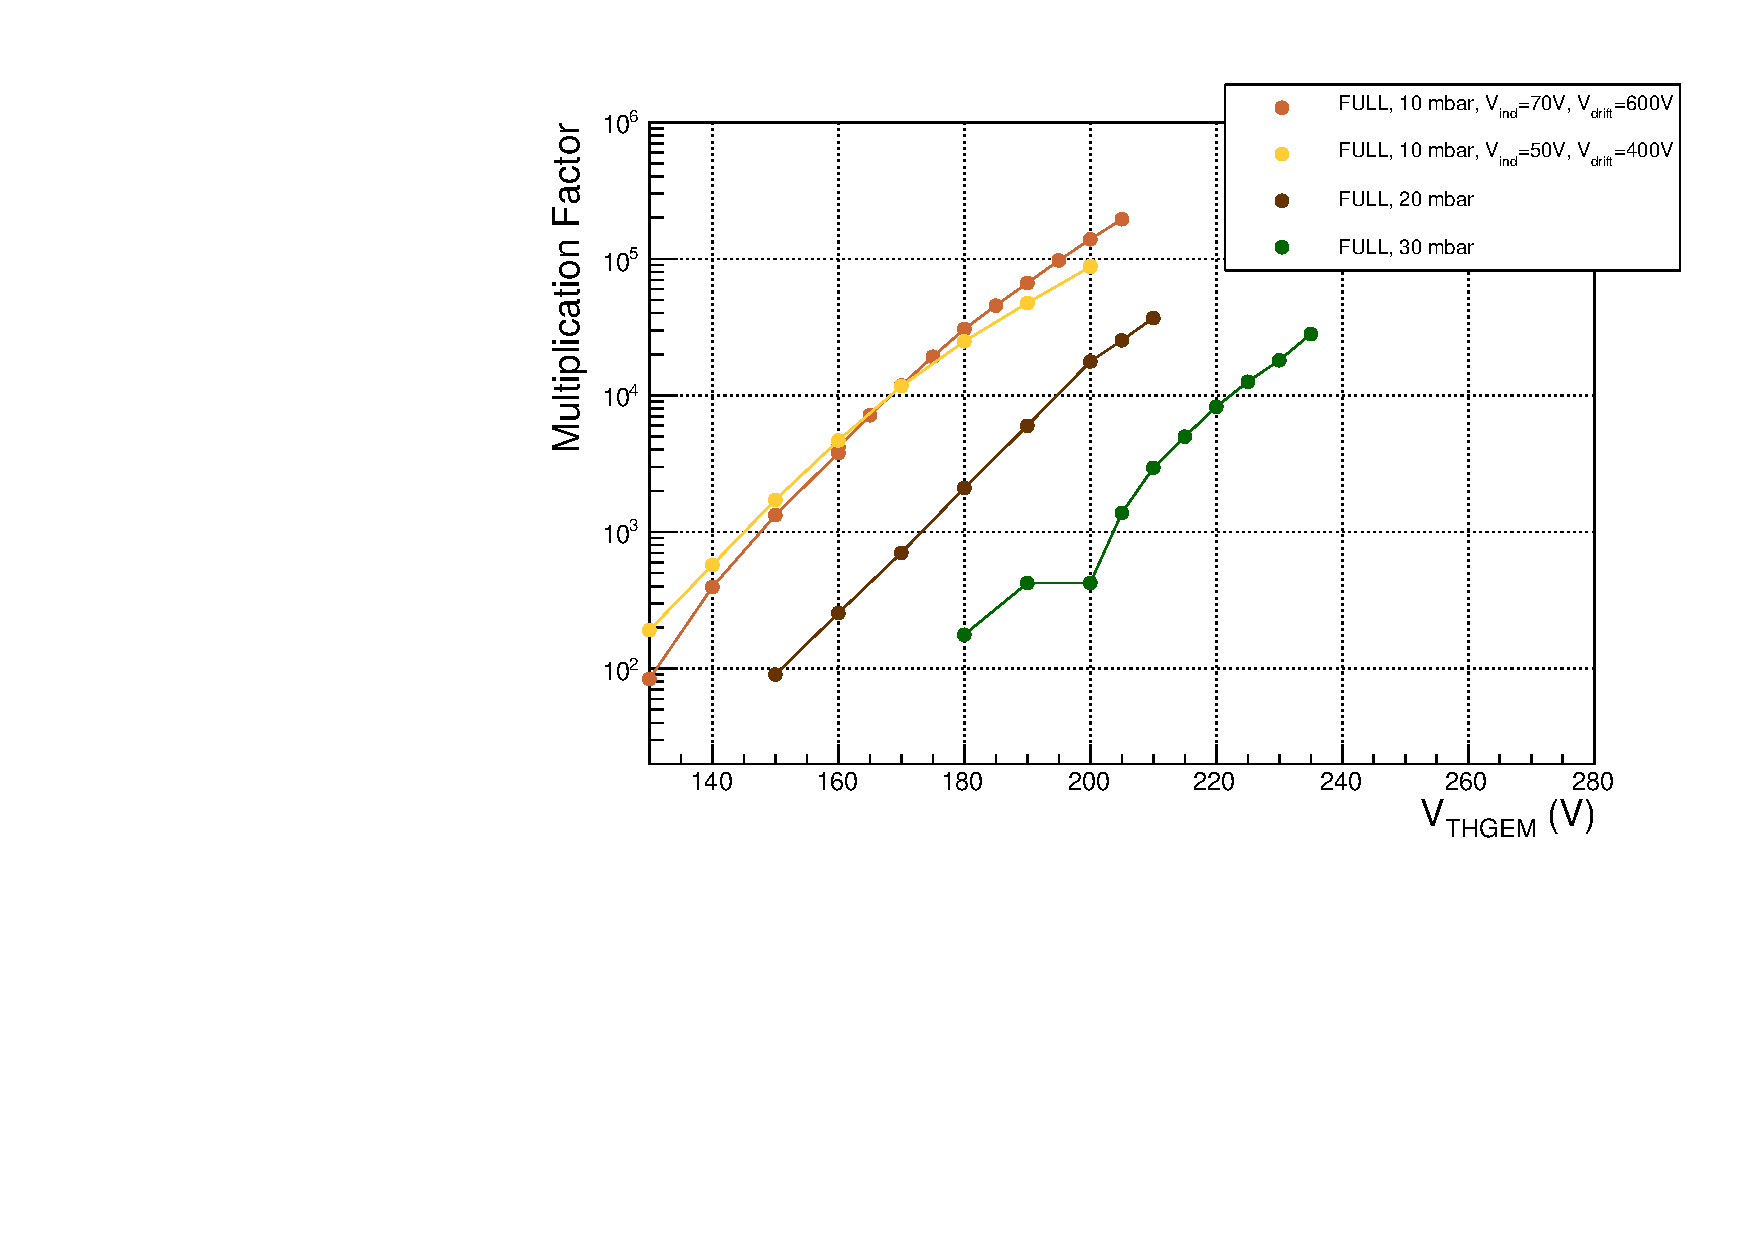
\includegraphics[width=\textwidth]{Immagini/MFvsTHGEM_FULL_bis.pdf}
	\caption{The multiplication factors evaluated for the FULL THGEM as a function of \Vthgem{} and pressure.}
	\label{fig:multiplication_factor_FULL_bis}
\end{figure}




\clearpage

\subsubsection{Scan on \Vdrift}

%The currents measured during \Vdrift{} scan have the same behavior (almost constant) of previous test. The difference is the current values, a clear example can be anodic current: ~0.5 nA fixing \Vind{} = 50 V and \Vthgem{} = 160 V and ~11 nA fixing \Vind{} = 70 V and \Vthgem{} = 190 V.

The new scan on \Vdrift{} was conducted fixing P~=~9.3~mbar, \Vind{} = 50 V and \Vthgem{} = 160 V.
%The measured currents have the same behaviour (almost constant) of the previous tests. 
Comparing this scan with a previous one done in similar conditions (P~=~11~mbar, \Vind{} = 70 V, \Vdrift{} = 600 V), which is shown in Figure~\ref{fig:drift_FULLTHGEM_11mbar}, the measured currents exhibit the same behaviour (almost constant).


\begin{figure}[htbp]
	\centering
	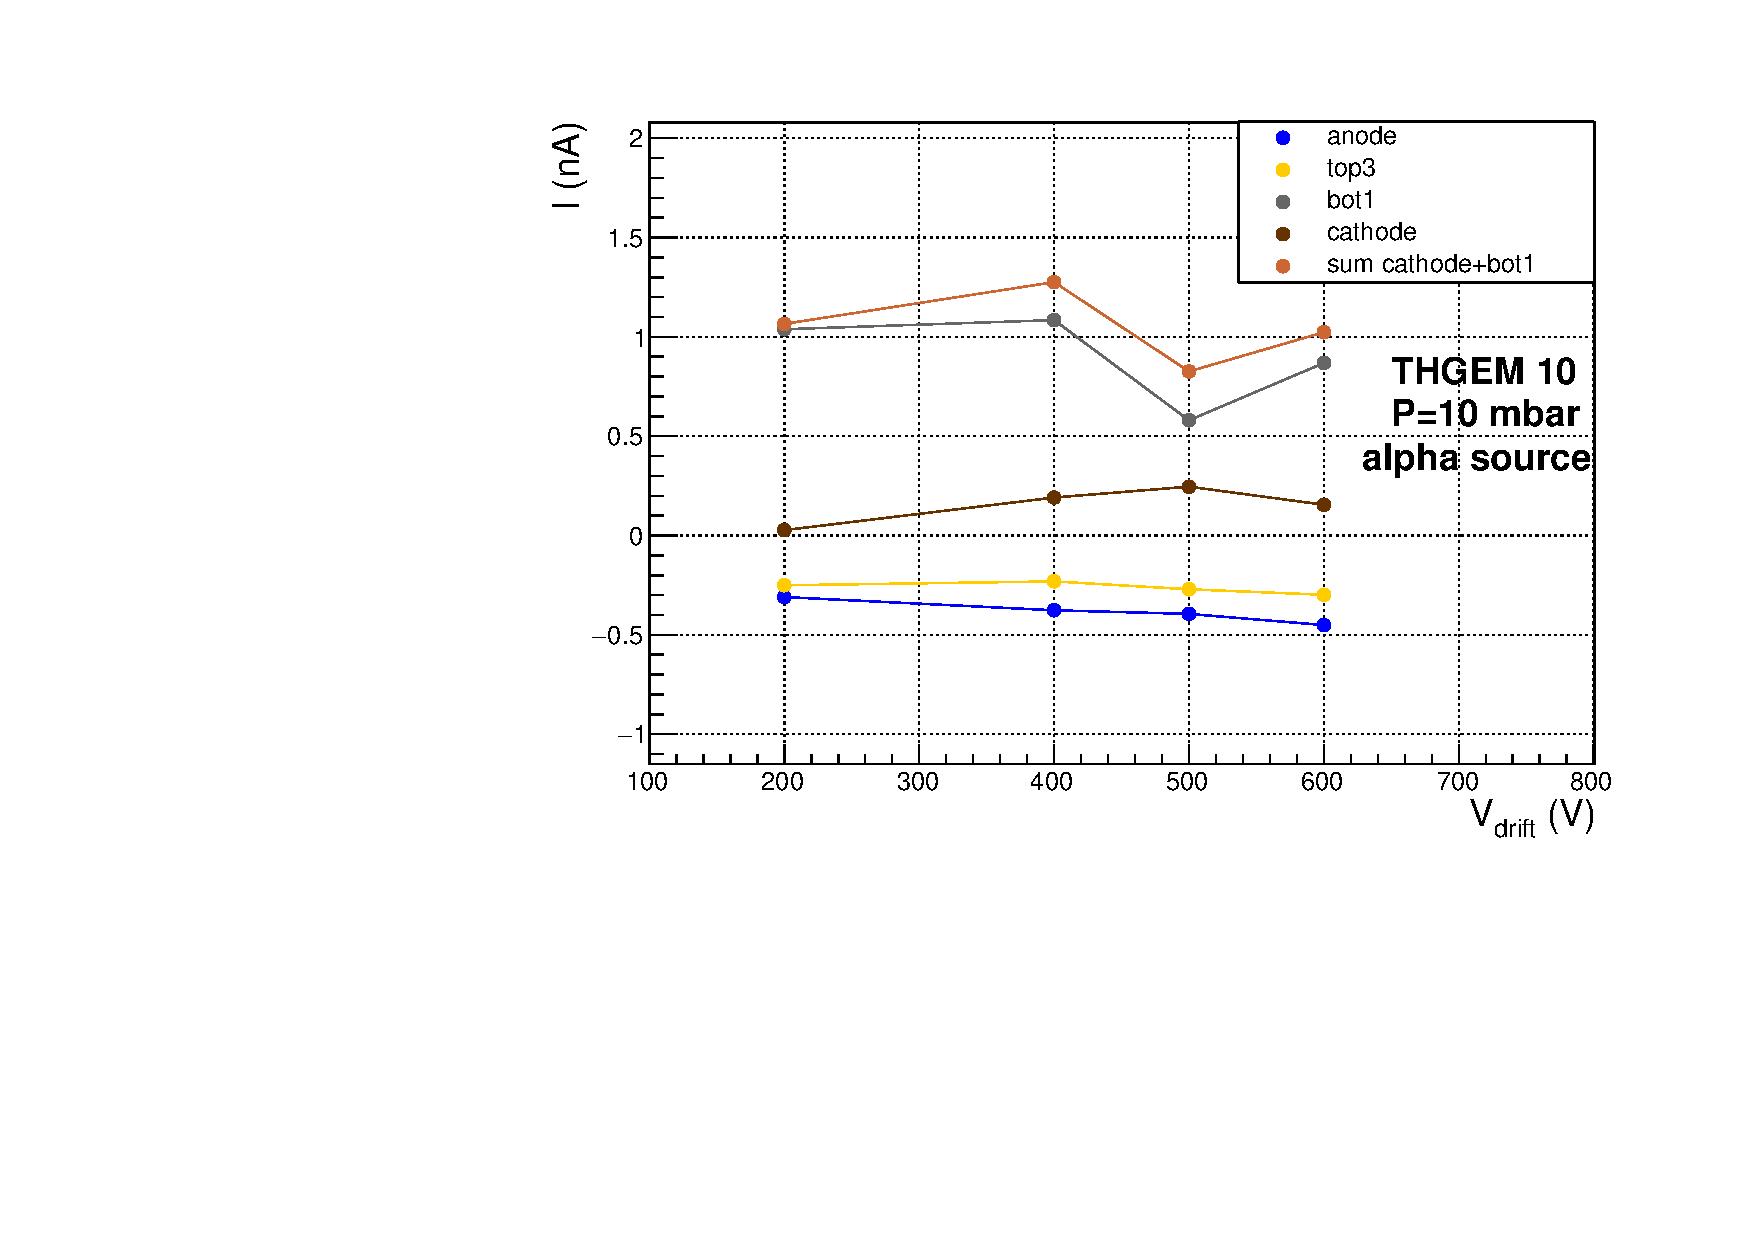
\includegraphics[width=\textwidth]{Immagini/driftScan_THGEM10_alpha_10mbar.pdf}
	\caption{Currents measured during the scan on the voltage \Vdrift{} across the drift region at 10~mbar.}
	\label{fig:driftScan_THGEM10_alpha_10mbar}
\end{figure}









\clearpage

\subsection{First test with beam} \label{sec:test_beam}

The first test with beam was done on February 19 2020. 
The prototype have been tested in the TeBe gas chamber that has an angle of 30$^{\circ}$ 
respect to the beam line direction (0$^{\circ}$). 
A beam of $^{18}$O at an energy of 16.5 MeV have been sent on a target of $^{116}$Cd xxx $\mu$.
Due to the high energy of the beam the number of particles reaching the tracker prototype
(that is a 30$^{\circ}$ respect to the beam direction),their mass charge and energy is not known.
The only information we have is the current read on the faraday cup FC4 that is 
along the TeBe beam line before the beam line gate valve. Therefore we can study how
the behaviour of the tracker scale with the current but we do not have 
a clear way to compare such results with the information coming from test with the $\alpha$-source.

One way to compare such results with the alpha's is to compare directly the 
anodic current.
Being equal all the parameters of the tracker (that is: P, \Vthgem{}, \Vind{}, \Vdrift{}),
it should manifest the same behaviour if the total charge produced is the same, even if the 
rate of particles entering the tracker is different.
In fact even if the same current on the anode can be generate by a very different rates 
of particles or heavy ions\footnote{Ion with different Z, M and energies loose quite different
amount of energy\ldots} the effects on the tracker are mainly linked to the total amount of 
charge produced and not on the rate of the particle\footnote{This is just partially thru. In fact 
this is valid because we are measuring currents, it is no more if we study the signal on the 
single strip of the anode. Moreover it is no strictly thru because there is a difference if
the total primary charge is produced at very low rate with event that generate a lot of charge
ore if the same total charge is produced at very high rate in events where a very small amount of 
charge is produced}.

Firstly the tracker was tested  at two values of the beam current 60 pA and 400 pA.
In order to increase the beam current a collimator was remove from the beam line. In this way 
we reached much higher values of the beam current: 1, 1.8 nA. Anyway since the 
optic of the beam is not the same, that is the beam could reach the target with a different 
emittance, is not correct to compare the first two beam currents
with the second two\footnote{For example if the emittance of the beam was the same we can
assert that with a beam of 1 nA we had a rate on the tracker that i s 2.5 times ahigher,
since the emittance is not the same is not correct to affirm this, moreover also 
the energy and Z of the particle reaching the tracker could be different.}

An important difference respect to the case of the $\alpha$-source test is that the rate
of the $\alpha$ particles is constant with a good approximation, the rate of the
particle reaching the tracker in the in-beam test is not constant but fluctuate
as the beam intensity.
The fluctuation occur during the measurements of the currents, that is during the 1-2 minutes
during which we take the average of the current and among one measurements and the others.
Therefore the plot with beam are less precise and suffers the effect of the fluctuation.
Unfortunately such uncertainty are not easy to extimate.

The pressure of isobutane was 9.4 mbar.

\subsubsection{Scan on \Vthgem}

The measurement was done at \Vind{} = 50~V and \Vdrift{} = 400~V with I$_{beam}$ 60 and 400 pA. 
The plots of the currents vs \Vthgem are shown in Figure~\ref{fig:thgemScan_THGEM10_beam_10mbar}.
The plots show have the same behaviour of the scan on \Vthgem{} with $\alpha$ source (see Figure~\ref{fig:thgem_FULLTHGEM_10mbar_bis}). 

The discharge occurred at \Vthgem{} = 190 V with both beam intensities, to be compared with \Vthgem{} = 210~V for the $\alpha$ case. 
%Another important difference is the maximum achievable anodic current: $\sim -$20 nA with $\alpha$ source, $\sim$120 nA with \ibeam = 60 pA and $\sim -$280 nA with \ibeam = 400 pA.

\begin{figure}[!htb]
	\centering
	\subfigure[]{ \label{fig:thgemScan_THGEM10_60pA_10mbar} 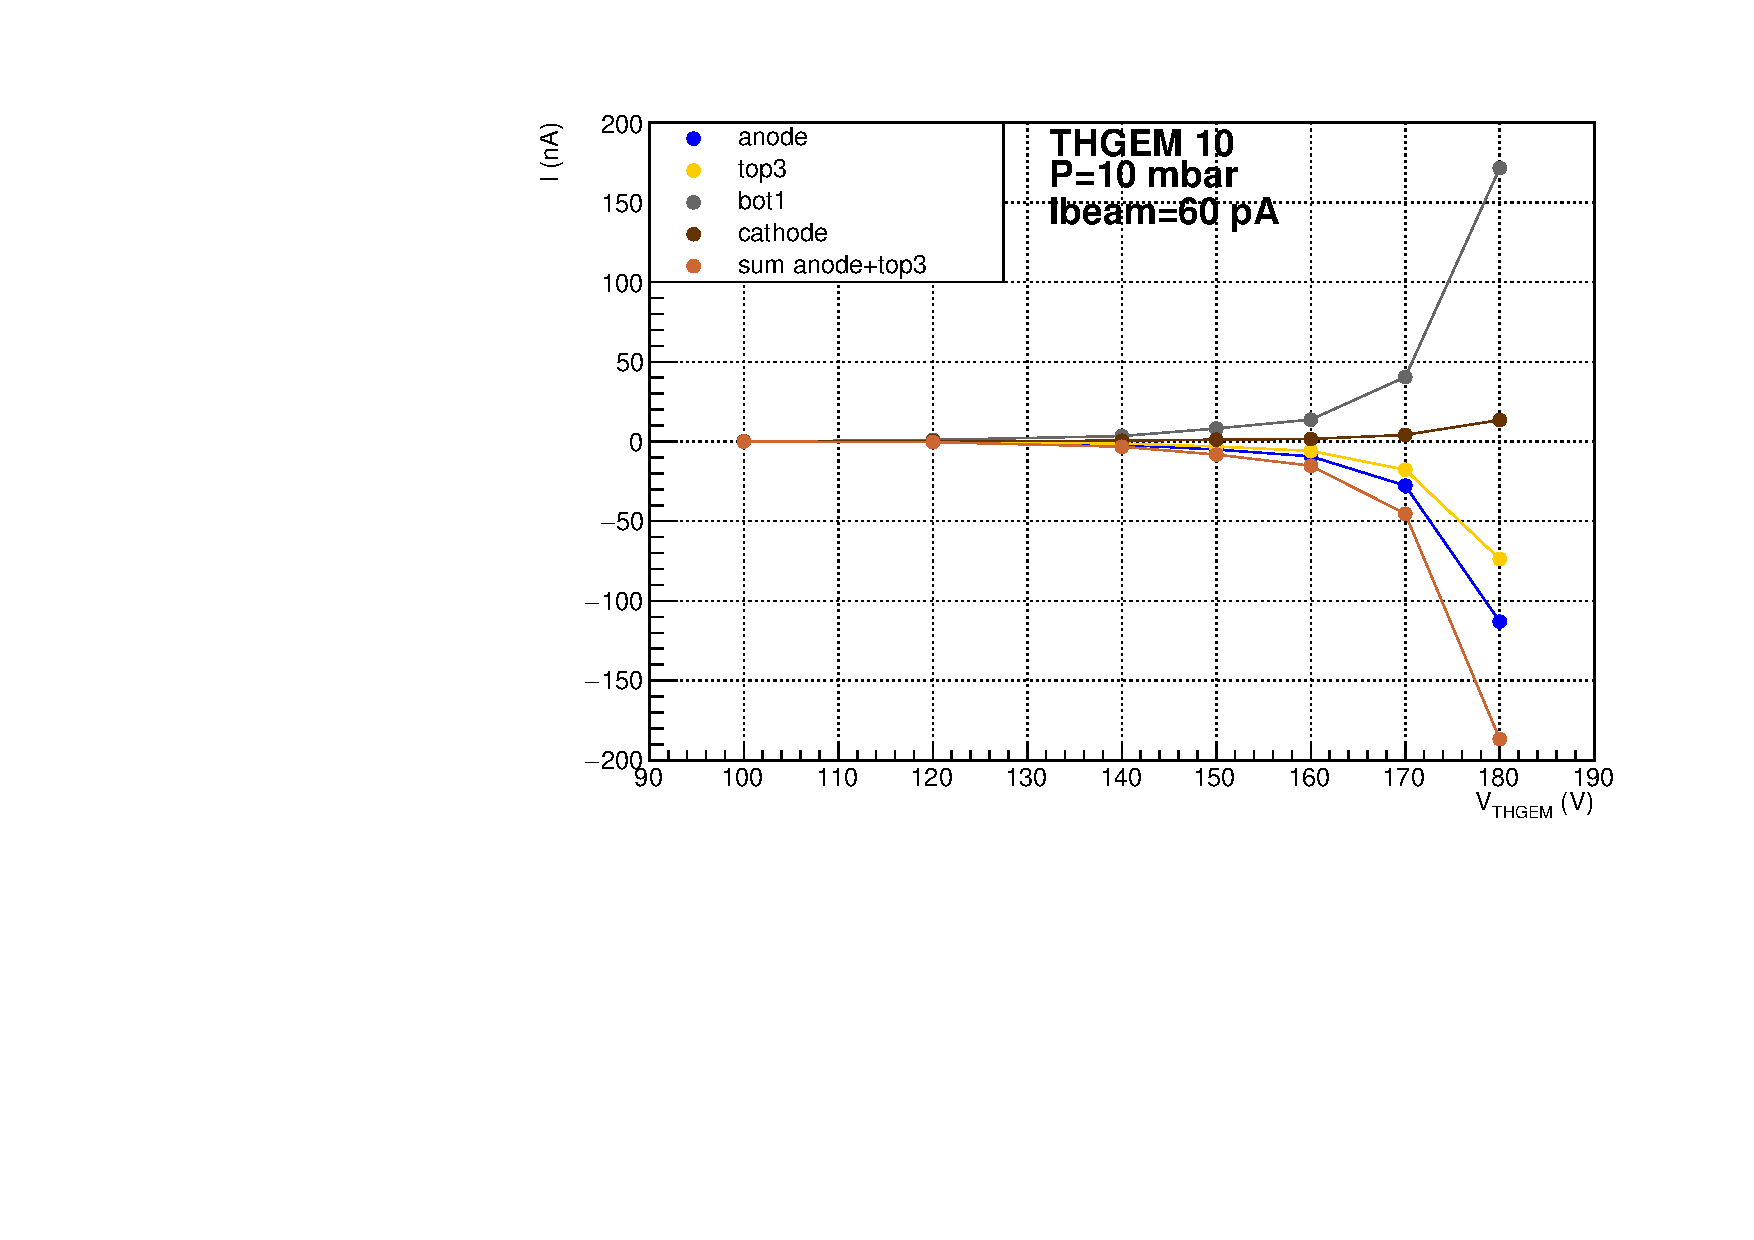
\includegraphics[width=0.96\textwidth]{Immagini/thgemScan_THGEM10_60pA_10mbar.pdf}}
	\subfigure[]{ 	\label{fig:thgemScan_THGEM10_400pA_10mbar} 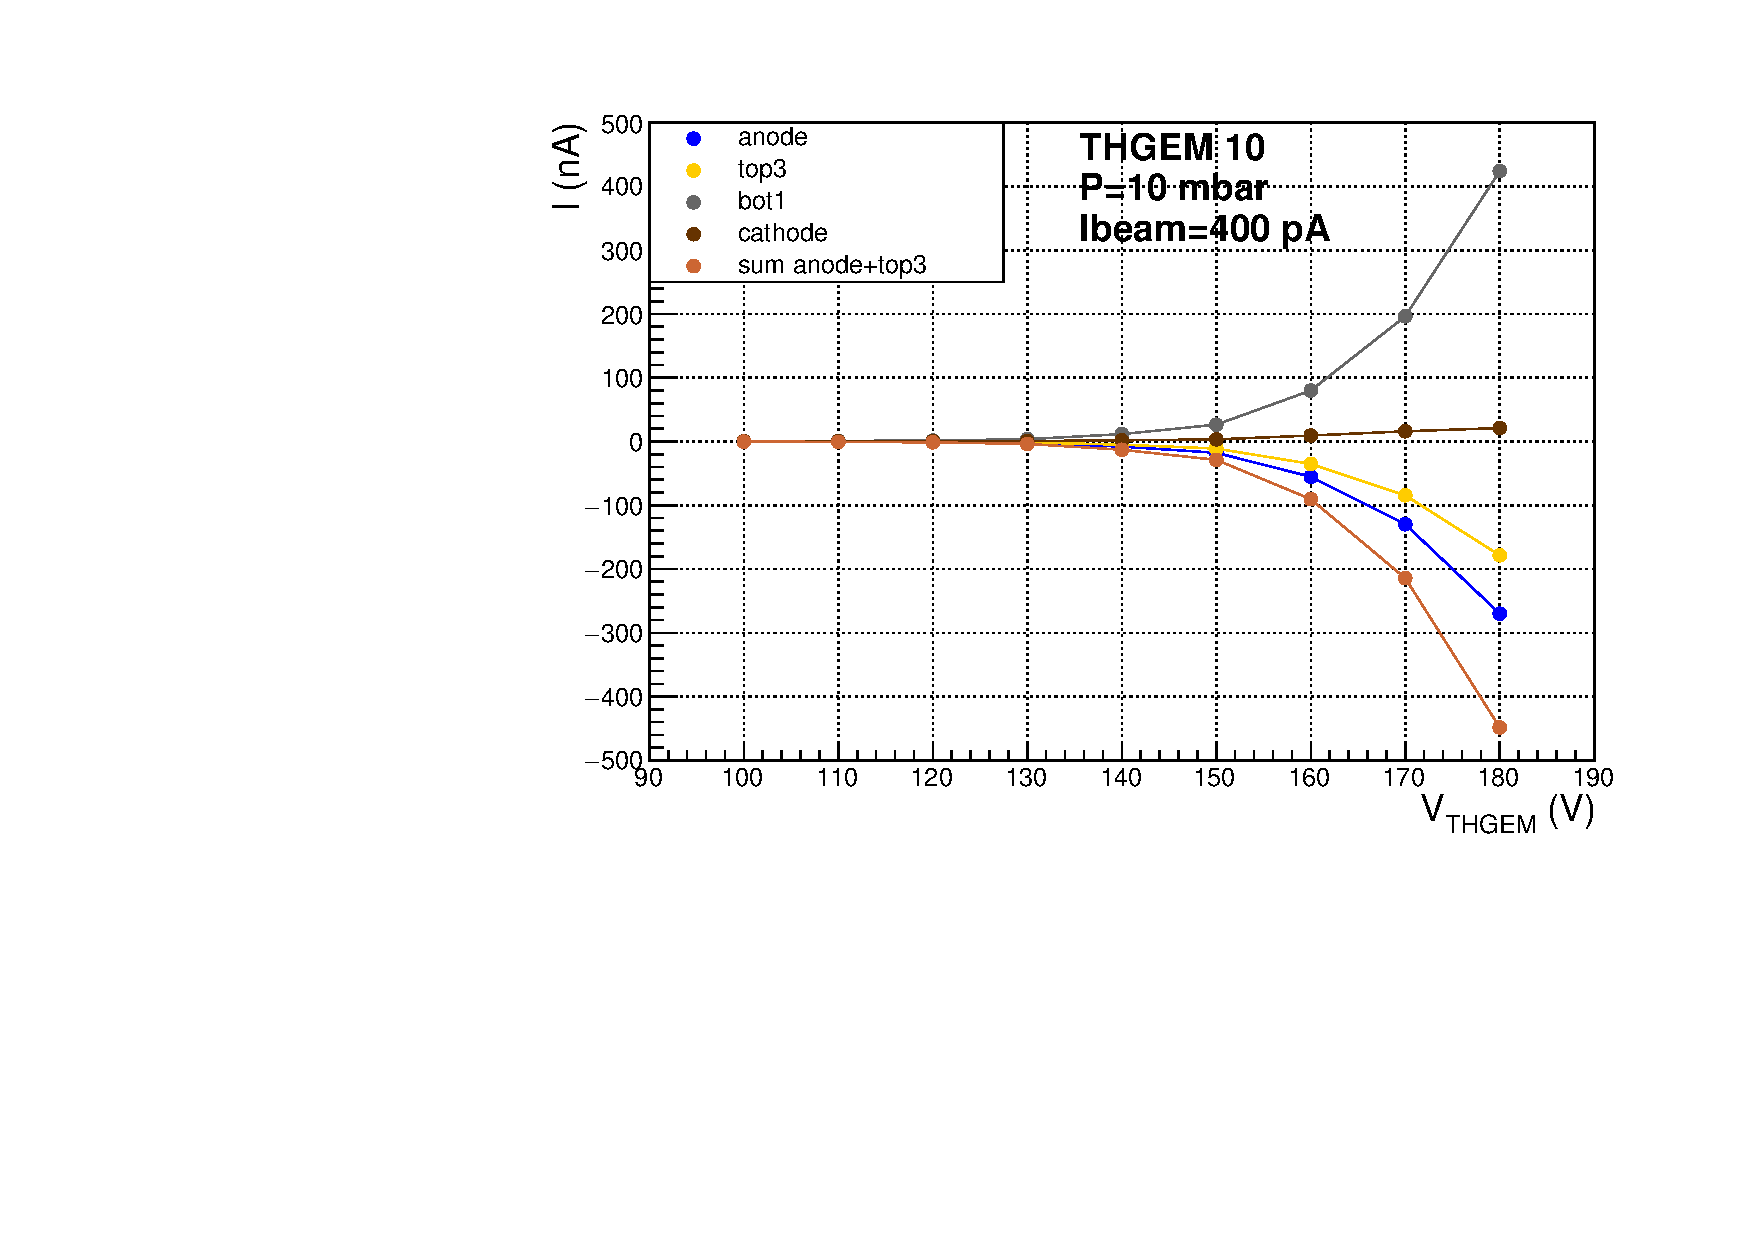
\includegraphics[width=0.96\textwidth]{Immagini/thgemScan_THGEM10_400pA_10mbar.pdf}}
	\caption{Currents measured during the scan on the voltage \Vthgem{} across each FULL THGEM fixing \Vind{} = 50 V and \Vdrift{} = 400 V: in (a) at 60 pA, in (b) at 400 pA.}
	\label{fig:thgemScan_THGEM10_beam_10mbar}
\end{figure}

%\clearpage

\subsubsection{Scan on \Vdrift}

The measurement was done fixing \Vind{} = 50~V and \Vthgem{} = 160~V. 
The plots of the currents vs \Vthgem are shown in Figure~\ref{fig:driftScan_THGEM10_beam_10mbar}.
The currents have the same behaviour of the scan on \Vdrift{} with $\alpha$ source (see Figure~\ref{fig:driftScan_THGEM10_alpha_10mbar}). 
The discharge voltage was 800 V with both beam intensities to be compared with about 750~V for the $\alpha$ source. Therefore, apparently there is no difference on the discharge voltage between the two cases
$\alpha$-spurce, beam.
%Another important difference is the maximum anodic achievable current: $\sim - $0.5 nA with $\alpha$ source, $\sim - $20~nA with \ibeam = 60~pA and $\sim - $55~nA with \ibeam = 400 pA.

\begin{figure}[!htb]
	\centering
	\subfigure[]{ \label{fig:driftScan_THGEM10_60pA_10mbar} 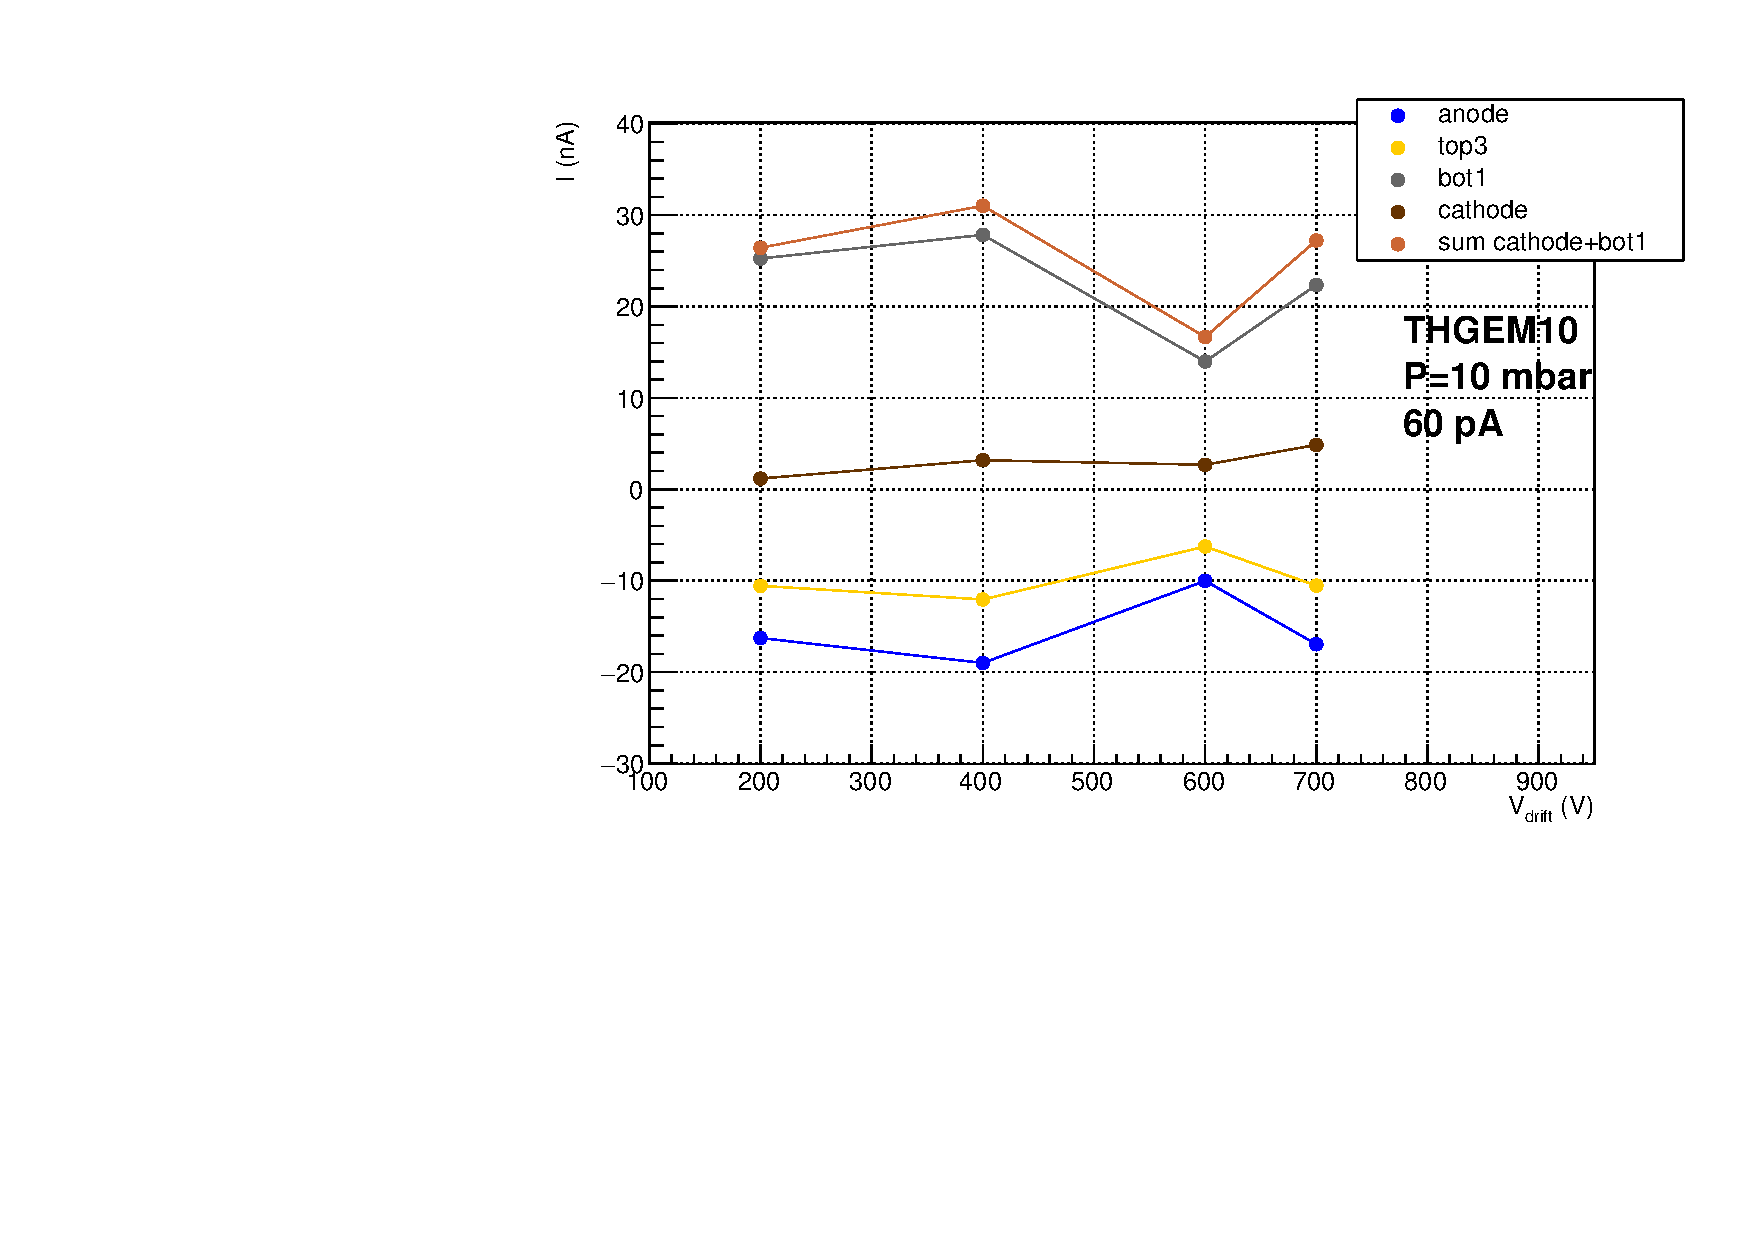
\includegraphics[width=0.96\textwidth]{Immagini/driftScan_THGEM10_60pA_10mbar.pdf}}
	\subfigure[]{ 	\label{fig:driftScan_THGEM10_400pA_10mbar} 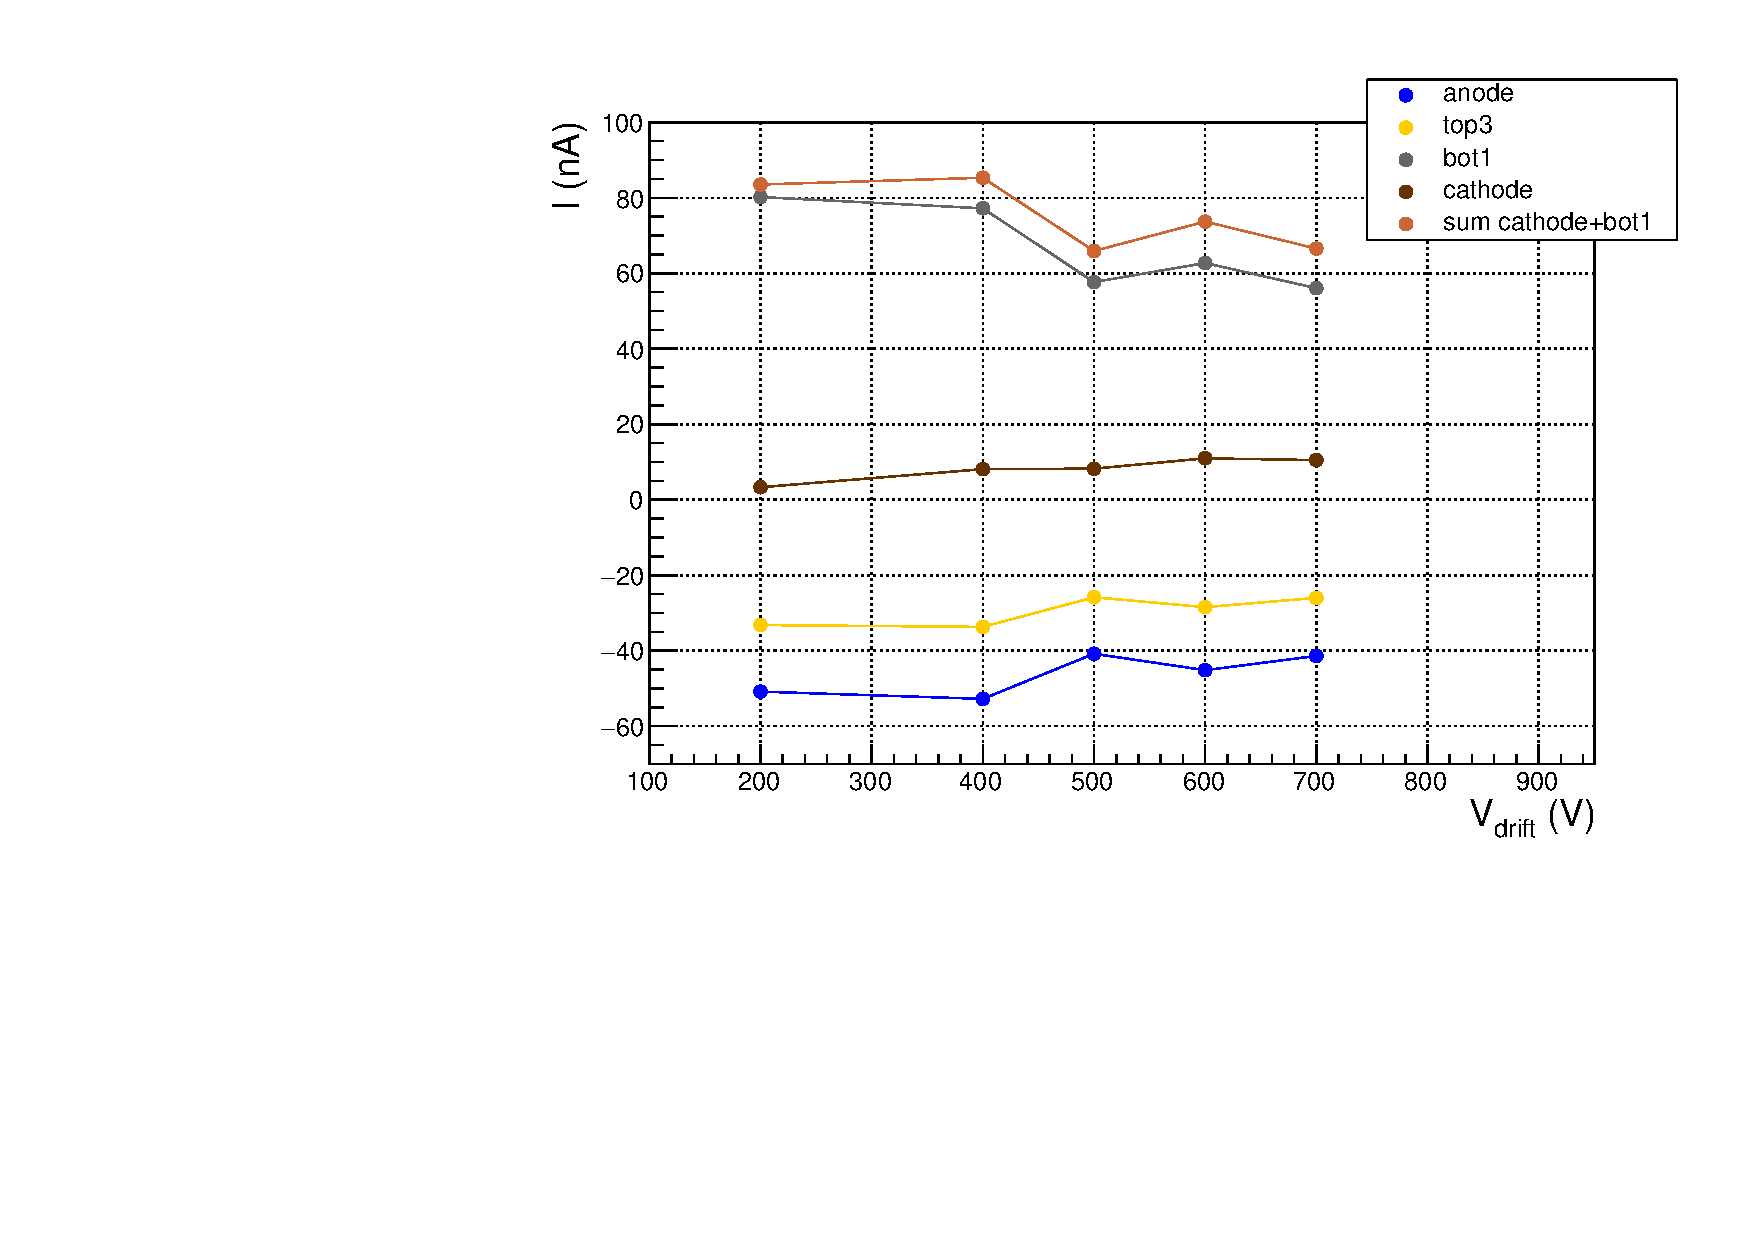
\includegraphics[width=0.96\textwidth]{Immagini/driftScan_THGEM10_400pA_10mbar.pdf}}
	\caption{Currents measured during the scan on the voltage \Vdrift{} across each FULL THGEM fixing \Vind{} = 50 V and \Vthgem{} = 160 V: in (a) at 60 pA, in (b) at 400 pA.}
	\label{fig:driftScan_THGEM10_beam_10mbar}
\end{figure}


%\clearpage

\subsubsection{Ion Backflow (IBF)}

Figure~\ref{fig:IBFvsDrift_withBeam} shows the IBF calculations as a function of \Vdrift{} for \ibeam{} equal to 60 and 400~pA.
Comparing the two curves we can affirm that there are no significant differences of the
IBF for the two beam currents. 
%Looking at Figure~\ref{fig:IBFvsDrift_withBeam} we can evaluate IBF behaviour increasing \Vdrift{}. 
%IBF linearly increases until \Vdrift{} = 600~V. After this point it seems to get a plateau but to be sure further measurements are needed.\\

\begin{figure}[htbp]
	\centering
	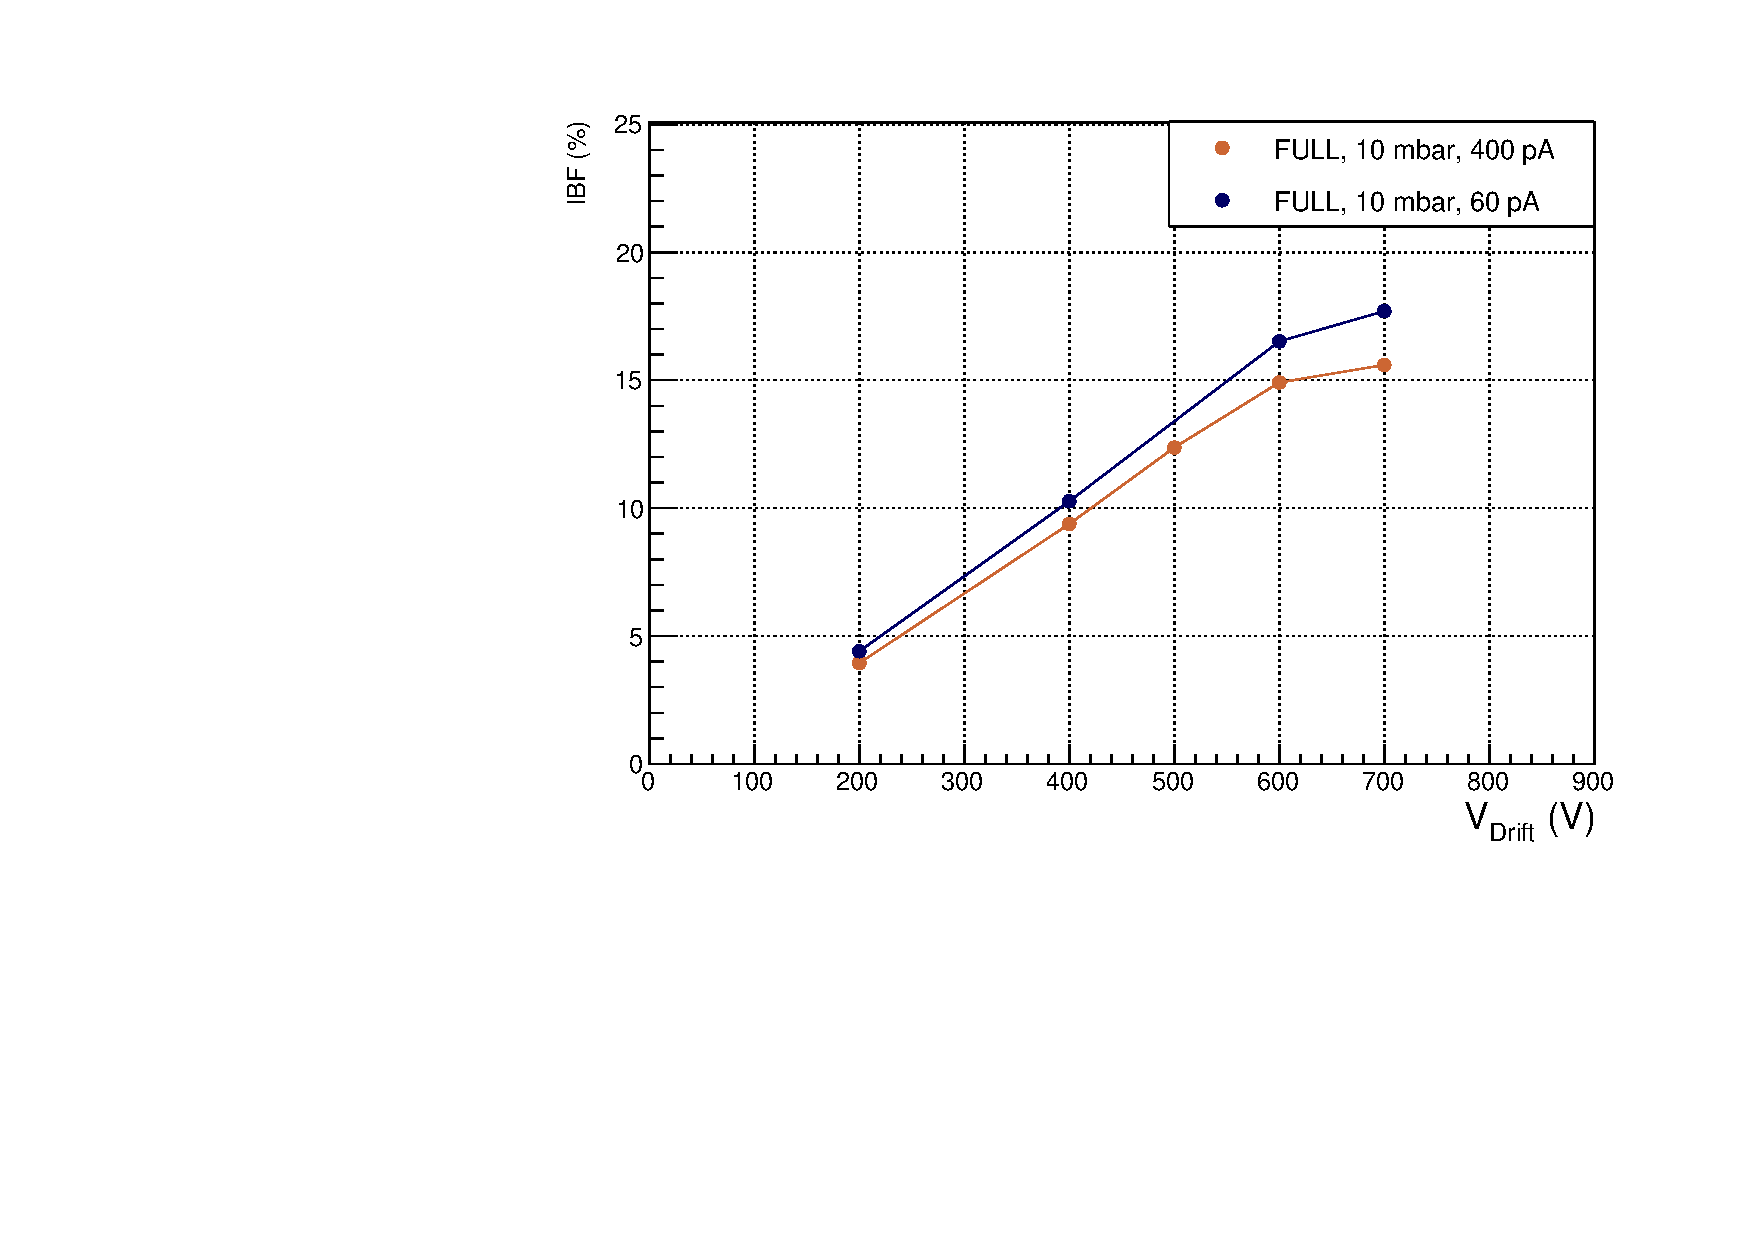
\includegraphics[width=\textwidth]{Immagini/IBFvsDrift_withBeam.pdf}
	\caption{Ion backflow evaluated for FULL THGEM as a function of \Vdrift{} at 60 pA and 400 pA fixing \Vind{} = 50 V and \Vthgem{} = 160 V.}
	\label{fig:IBFvsDrift_withBeam}
\end{figure}

%In Figure~\ref{fig:IBFvsDrift_beam_alpha_average}, IBF was studied as a function of \Vdrift{}. 
Figure~\ref{fig:IBFvsDrift_beam_alpha_average} shows a comparison between the IBFs with $\alpha$ 
source and those with beam. 
%The IBF for 60 pA, 400 pA at \Vthgem{} = 160 V and $\alpha$ source  at \Vthgem{} = 190 V has a maximum IBF of 17\%. 
%In the test with $\alpha$ source, when \Vthgem{} is less than 190 V the cathode current is so small 
%that IBF estimate is not reliable. 
IBF as a function of \Vdrift{} seems not sensible to the rate because the curves are basically the same
for beam and alpha-source.
%This is not well understood.
There are also few points taken at different value of beam currents but at a single value of \Vdrift.
The trnd seems that increasing the beam current and fixing all the other parameters, the IBF decreases. 
This effect anyway is not so clear and could be simply due to the large uncertainties of the 
measurements.
%This behaviour cannot be explained. 
%Looking at the blue and red circle points, IBF decreases with increasing \Vthgem.\\

\begin{figure}[htbp]
	\centering
	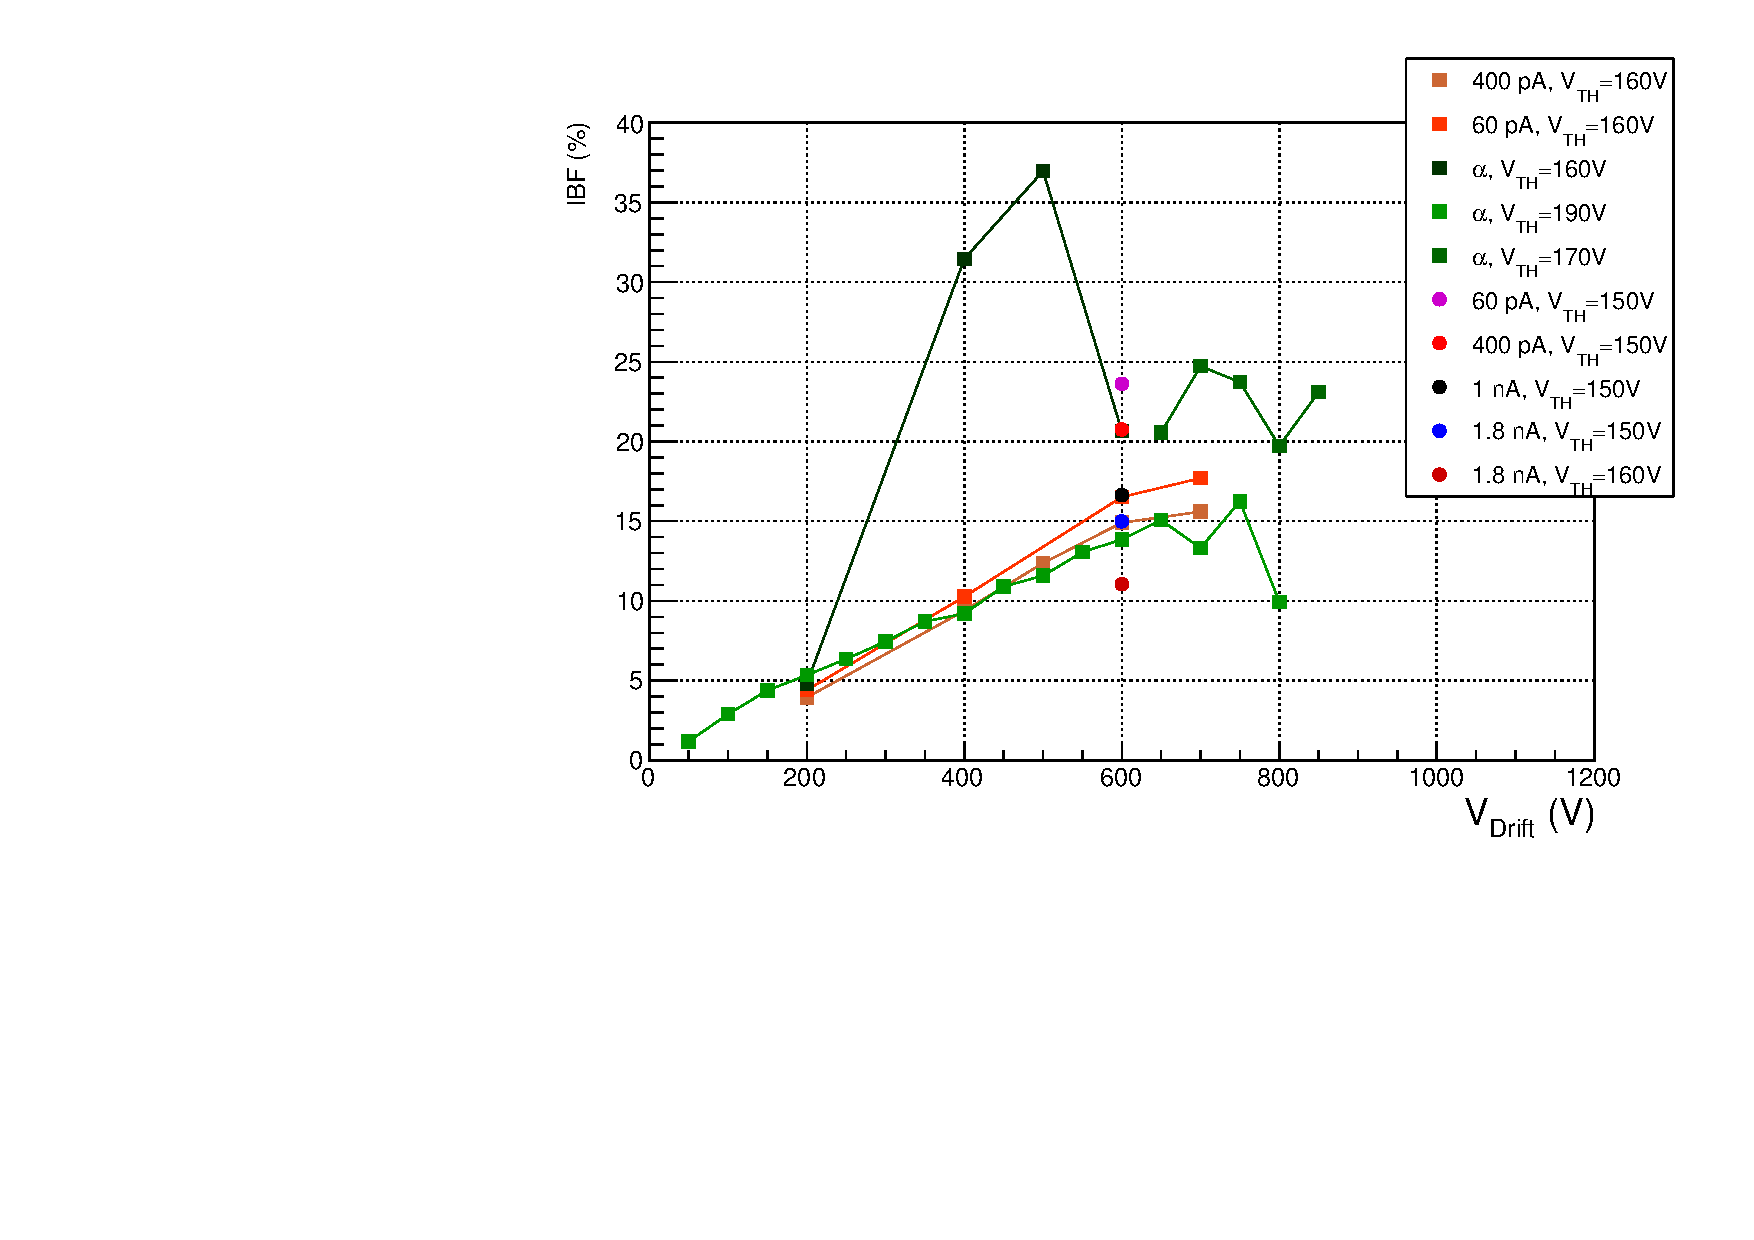
\includegraphics[width=\textwidth]{Immagini/IBFvsDrift_beam_alpha_average.pdf}
	\caption{Ion backflow evaluated for FULL THGEM as a function of \Vdrift{} at 60 pA, 400 pA, 1 nA, 1.8 nA and with $\alpha$ source.}
	\label{fig:IBFvsDrift_beam_alpha_average}
\end{figure}

IBF was studied also as a function of \Vthgem: the results are shown in Figure~\ref{fig:IBFvsTHGEM_beam_alpha}. 
%From \Vthgem{} = 100 V to \Vthgem{} = 140 V, IBF decreases rapidly, between \Vthgem{} = 140 V and \Vthgem{} = 205 V IBF is nearly constant.
IBF is nearly constant with varying \Vthgem.
The best condition to have IBF as less as possible is to work near \Vthgem{} = 200 V but as far as possible from discharge.\\


\begin{figure}[!p]
	\centering
    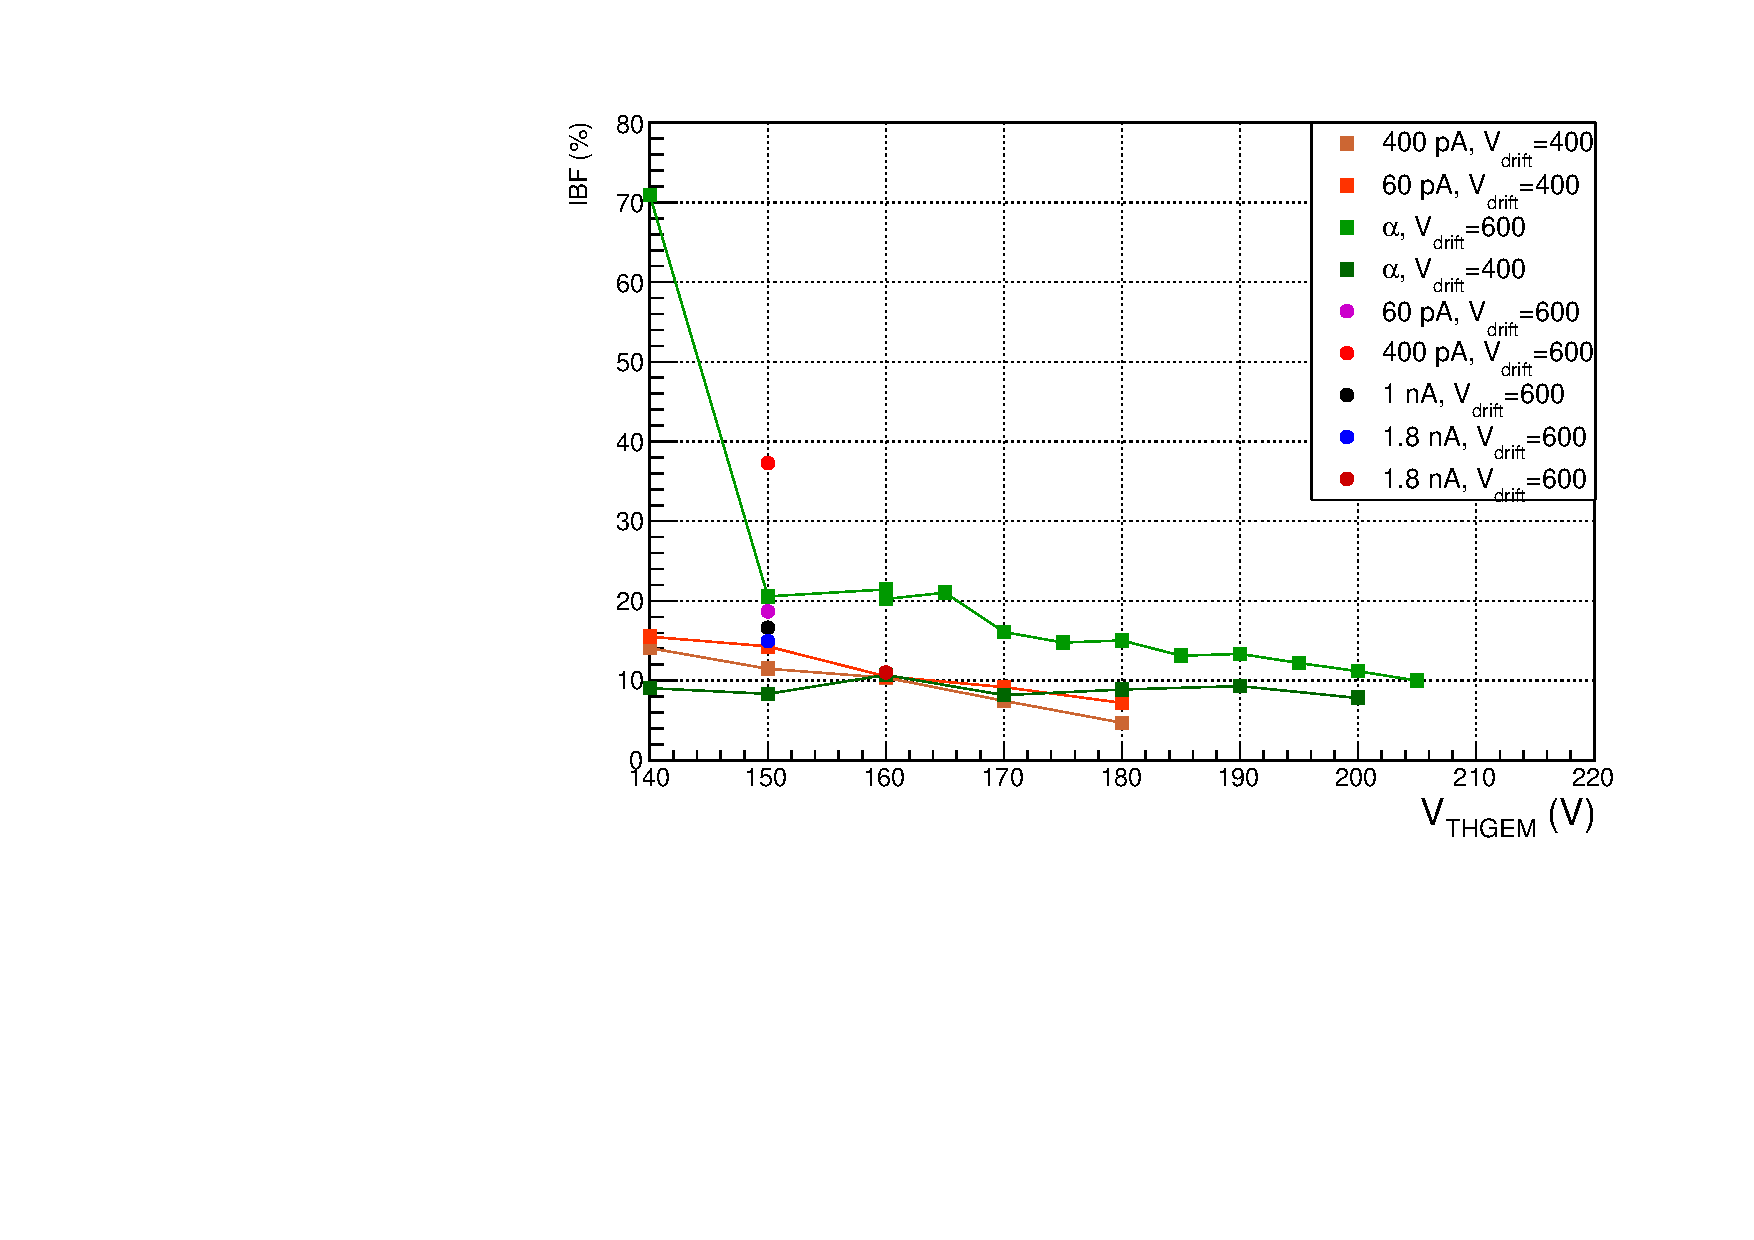
\includegraphics[width=1.\textwidth]{Immagini/IBFvsTHGEM_beam_alpha_zoom.pdf}
	\caption{Ion backflow evaluated for FULL THGEM as a function of \Vthgem{} at 60 pA, 400 pA, 1 nA, 1.8 and with $\alpha$ source.}
	\label{fig:IBFvsTHGEM_beam_alpha}
\end{figure}


IBF was studied also as a function of \Vind: the results are shown in Figure~\ref{fig:IBFvsInd_beam}. 
As already said, IBF for ROW THGEM is much bigger than that for FULL THGEM.
Another difference is that IBF is constant for FULL THGEM and it decreases for ROW THGEM. 
IBF is not dependent on pressure and it maybe decreases with increasing beam current.

\begin{figure}[!t]
	\centering
	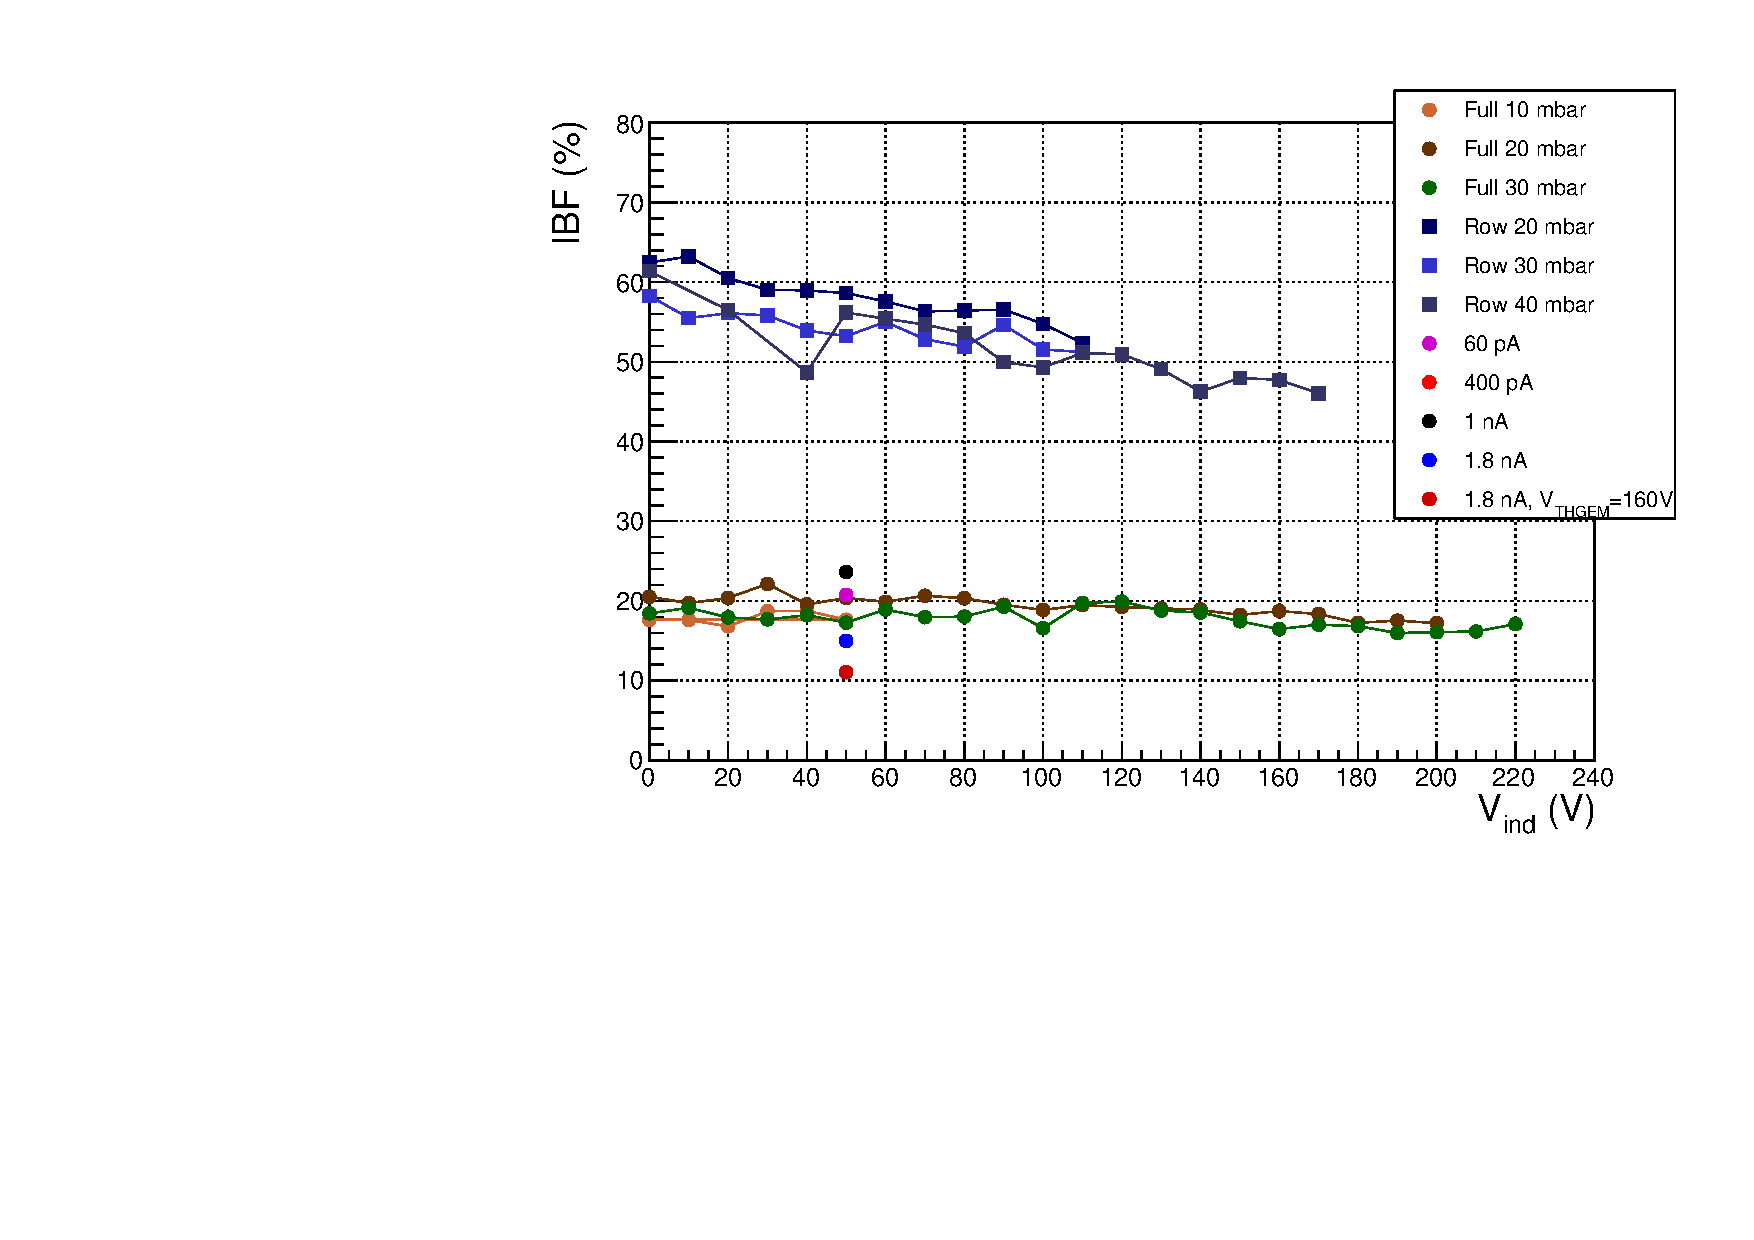
\includegraphics[width=\textwidth]{Immagini/IBFvsInd_beam.pdf}
	\caption{Ion backflow evaluated for FULL THGEM as a function of \Vind{} at 60 pA, 400 pA, 1 nA, 1.8 nA and with $\alpha$ source.}
	\label{fig:IBFvsInd_beam}
\end{figure}


\subsubsection{Scan on the rate}

\textcolor{red}{Ha senso mettere questa parte?}\\
In Figure~\ref{fig:IbeamScan_THGEM10_10mbar_average} the measured currents were plotted as a function of the beam current (\ibeam). 
%We expected a linear behaviour, but instead we found an exponential one. This behaviour can be explained because the point at 60 pA and 400 pA have different conditions from the others. 
It is important to remember the discussion done at the beginnign of the section
that is that the points at 1 and 1.8 nA where obtained with a beam that had
a difference emittance respect to the point at 60 and 400 pA.
Therefore the scaling of the rate from the first tow points to the second two is not correct.


\begin{figure}[htbp]
	\centering
	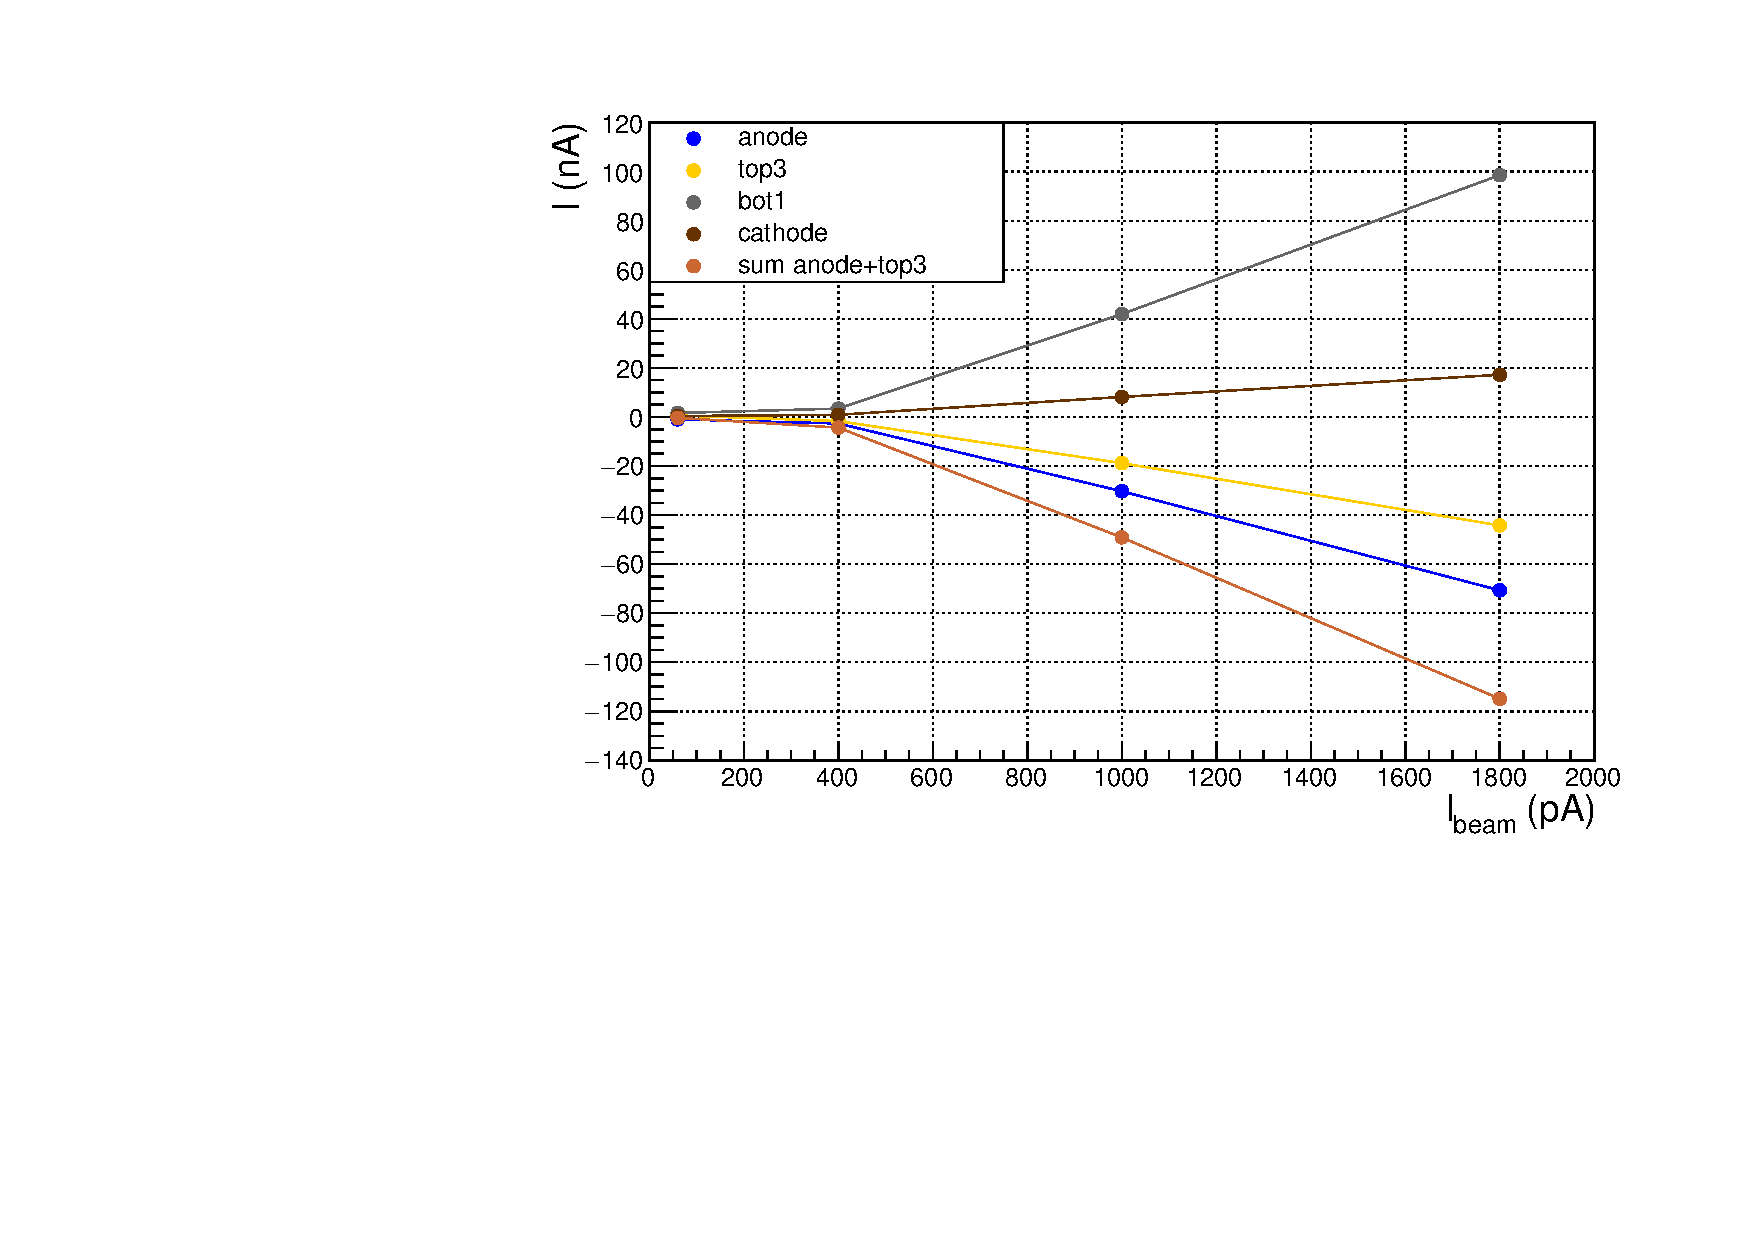
\includegraphics[width=\textwidth]{Immagini/IbeamScan_THGEM10_10mbar_average.pdf}
	\caption{Currents measured with varying \ibeam.}
	\label{fig:IbeamScan_THGEM10_10mbar_average}
\end{figure}

%\section*{Notes}

%partiamo dalle full thgem:

%sulla parte di induzione: uno dei grafici con i quattro canali e la somma appropriata, incrocio fra corrente anodo e top3, regione di quasi plateau, poi la corrente aumenta, se avremo delle simulazione potremo corredare il discorso; obiettivo: cercare la regione di migliore funzionamento che dovrebbe essere quella del plateau



%sulla parte delle thgem: andamento esponenziale, si raggiunge il limite di scarica, non sappiamo se la scarica \E8 nelle thgem



%sulla parte di drift: variare la corrente tra catodo e bottom1; a 0 volt abbiamo una misura: o lo strumento segna zero ma non \E8 zerp 


%%descrizione delle varie pressioni: un grafico tenendo soltanto anodo a diverse pressioni, questo grafico non varia drammaticamente al variare della pressione; un altro grafico con l'induzione al variare della tensione delle thgem e/o del drift.



%%ion backflow: calcolare direttamente il valore in percentuale; unico grafico al variare delle pressioni; esso non dipende molto dall'induzione; esso dipende anche delle thgem (configurazione delle linee di forza); conclusione: 

%%fattore di moltiplicazione: inizialmente solo con le thgem piene;
%%poi thgem row e mostrare i tre grafici esemplificativi
%%induzione delle row thgem a 20 mbar \E8 pi\F9 bello;

%\subsection{ROW THGEM}

%%la drift \E8 da discutere: la loro geometria \E8 diversa: 5 fila isolate e proviamo a spiegare che a basse tensioni della drift, il campo elettrico delle thgem forma un imbuto pi\F9 largo, se vdrift aumenta la regione da cui le thgem raccolgono carica diminuisce

%%dalle row thgem ci aspettiamo meno corrente perch\E9 hanno meno buchi: invece di 143 file, ne hanno 5, quindi hanno il 3.5\% dei buchi rispetto a quelle piene. In prima approssimazione potremmo aspettarci che il valore della corrente scali allo stesso modo. 

%%ion backflow nelle row \E8 sistematicamente pi\F9 alto; vediamo se l'andamento \E8 simile; al variare dell'induzione diminuzione dell'IBF; 

%ricordarsi di fare la misura del drift delle row a 20 mbar
%ATTENZIONE: altri test tenendo i campi elettrici fissi
%Misura ad alta pressione con full thgem, misura ad altre pressione con row thgem e rifare i test cercando di mantenere i campi elettrici costanti (possibilmente con il drift a tensioni basse)



%\section{Conclusioni}




\end{document}
